% -*- root: These.tex -*-
\graphicspath{{FigurePartie2/}}

\chapter{Réalisation d'une plateforme intégrée}

\startcontents[chapters]
\Mprintcontents

% -*- root: These.tex -*-

\Anotecontent{versionnerwf}{Par versionner on entend a minima la possible de  garder, de visualiser, de restaurer l'ensemble des modifications apportés à un fichier ou un ensemble de fichier. Les \textit{workflow} contiennent des données de natures très hétérogènes (modèles de simulation, bases de données, fichiers, etc.), ce qui rend le développement d'un outil capable de stocker et de restaurer intelligement un tel environnement dans ses différentes versions plus complexe à réaliser.}

\Anotecontent{ca_calibrage}{Cette littérature semble émerger, en géographie, plus vite dans le calibrage automatique des CA que dans la calibration des ABM.}

\Anotecontent{pom_realiste}{\foreigntextquote{english}[{\cite[315-316]{Railsback2012}}]{Let us warn you that no other platforms or ways to design and program ABMs are remotely as easy to use, well documented, and polished as Netlogo is. You can expect a serious increase in the effort and software knowledge required to produce working models, which could be a strong incentive to keep your models simple enough to stick with netlogo. However, if you do think you will outgrow NetLogo, we strongly recommend taking one or two serious courses in object-oriented programming, probably using the Java language.[...] Another alternative to consider seriously is finding a collaborator to provide the software expertise - either a paid programmer or an academic computer scientist (Chapter 8 of Grimm and Railsback 2005 provides advice on working with software professionals.)}}

\Anotecontent{paul_rationalite}{On parle aussi de rationalité procédurale dans le domaine de la cognition.}

\Anotecontent{uncertainty_grimm}{\foreigntextquote{english}[{\cite[255-256]{Railsback2012}}]{Parameterization is the word modelers used for the step of selecting values for a model's parameters.[...] The reason that parametrization is important is, of course, that quantitative results matter.[...] Calibration is a special kind of parameterization in which we find good values cause the model to reproduce patterns observed in the real system. Calibrating an ABM is part of POM because we calibrate \enquote{against} (i.e., to reproduce) patterns observed in the real system. Now, however, the patterns are typically quantitative instead of qualitative and more descriptive of the whole system, not its agents and parts. [...] Why do we include calibration as a part of pattern-oriented modeling separate from theory development, when they both include changing of adjusting a model until it adequately matches a set of observed patterns ? The major differences is that in theory development, we are focused on one particular part of a model: its traits for agent behavior. We often test theory against qualitative patterns so that we do not need to worry yet about how closely model reproduces observations from the real system. Calibration comes after we've identified theory for behavior and assembled the full model. Another way to think of the difference between this chapter and the rest of POM is that chapters 18 and 19 were about using patterns to reduce a model's \enquote{structural uncertainty} by finding good model designs and agent traits, and this chapter is about reducing \enquote{parameter uncertainty} by finding good parameter values.}}

\Anotecontent{evaludation}{\foreigntextquote{english}[\cite{Augusiak2014}]{Confusion about model validation is one of the main challenges in using ecological models for decision support, such as the regulation of pesticides. Decision makers need to know whether a model is a sufficiently good representation of its real counterpart and what criteria can be used to answer this question. Unclear terminology is one of the main obstacles to a good understanding of what model validation is, how it works, and what it can deliver. Therefore, we performed a literature review and derived a standard set of terms. ‘Validation’ was identified as a catch-all term, which is thus useless for any practical purpose. We introduce the term ‘evaludation’, a fusion of ‘evaluation’ and ‘validation’, to describe the entire process of assessing a model’s quality and reliability.}}

\Anotecontent{dsl}{Pour les modélisateurs, il faut imaginer que ce langage dédié met à disposition des utilisateurs différentes primitives spécifiques au logiciel pour construire et exécuter les \textit{workflows}, un peu comme Netlogo le propose avec la manipulation des Tortues.}

\Anotecontent{holland_multi_utilisation}{ Holland a développé les GA avant tout pour leur capacité de \foreignquote{english}{robust adaptive systems} et pas seulement pour leur capacité d'optimisation comme le rapelle \textcite{DeJong1993a} : \foreignquote{english}{However, with all this activity, there is a tendency to equate GAs with function optimization. There is a subtle but important difference between \enquote{GAs \textbf{as} function optimizers} and \enquote{GAs \textbf{are} function optimizers}} ; L'investissement d'Holland dans l'étude des \foreignquote{english}{Complex Adaptive Systems} s'inscrit dans une trajectoire de recherche resté proche des thématiques de ce qui deviendra plus tard la méta-discipline \textit{Artificial Life}. Son investissement continue dans cette branche de développement est d'ailleur lisible au travers de deux plateformes successive sur ce thème : \textit{$\alpha$-universe} et \textit{Echo} dont on trouve une analyse dans les travaux de \autocites{Taylor1999, Taylor2001} }


\Anotecontent{difference_objective_heuristique}{Il n'est pas forcément évident de faire la différence entre ces termes très proches, dont le sens se recoupe parfois, voici donc une aide à la désambiguisation inspirée de celle de \textcite[36]{Weise2011} :

\begin{enumerate}[labelindent=\parindent,leftmargin=*]
\item La fonction objectif (\textit{objective function}) peut etre considérée comme une forme d'heuristique, à la différence que celle ci est une mesure forcément directe du potentiel d'un aspect de la solution, alors que l'heuristique peut être de mesure directe ou indirecte, en ne fournissant par exemple qu'une approximation de la distance séparant une mesure de l'optimum. En ce sens, la fonction objectif mobilise souvent plus d'expertise sur le système que l'heuristique.
\item Une fonction \textit{fitness} est une fonction d'utilité secondaire, conçu comme une combinaison possible de fonction objectifs, et/ou d'heuristiques. Celle-ci peut également être une mesure relative, pour quantifier par exemple la différence existante entre deux solutions.
\end{enumerate}}

\Anotecontent{barricelli_multi_utilisation}{ Tout comme les travaux de McMillan ont permis de voir plus clair dans les intentions de Von Neumman derrière la notion de \textit{self-reproduction automata} ..., les travaux de Dyson \Autocite{Dyson1997}, de Fogel \autocite{Fogel2006a} sur l'histoire de cette discipline a permis également de redécouvrir les recherches de Barricelli comme celle d'un véritable pionnier en ALife, mais également comme celui d'un pionnier dans l'idée d'utiliser l'évolution comme support à la résolution de problème.}

\Anotecontent{fraser_comment}{\foreignquote{english}{Fraser was one of the first to conceive and execute computersimulations of genetic systems, and his efforts in the 1950s and1960s had a profound impact on computational models of evo-lutionary systems. The simulation algorithms he used were im-portant not only in the simulation of genetical problems, but pro-vided a menu of techniques that enriched the entire simulationeffort in any problem that involved probability sampling amonga population of alternatives, the heart of Monte Carlo methods. }\autocite[429]{Fogel2002}}

\Anotecontent{note_pattee_semantic_closure}{ \foreignquote{english}{Additionnary, from an epistemological point of view, Pattee(1995b) points out taht symbolic information (such as that contained in an organisms's genes) has \enquote{no instrinsic meaning outside the context of an entire symbol system as well as the material organization that constructs(writes) and interprets(reads) the symbol for a specific function, such a classification, control, construction, communication ...}. He argues that a necessary condition for an organism to be capable of creative open-ended evolution is that it encapsulates this entire self-referent organisation (Pattee refers to this condition as semantic closure). From this it follows that organisms should be constructed \enquote{with the parts and the laws of an artifical physical world} Pattee (1995a)(p.36). In other words, the interpretation (phenotype) of the symbolic information (genotype) of an artificial organism should be constructed and act within the artificial physical environment of the system. Additionally, if the system is to model the \enquote{origin} of genetic information, then the genotype itself must also be embedded within the environment; that is, the complete semantically-closed organisation -- the \enquote{entire organism} -- must be completely embedded within the physical environment.} \autocite{Taylor2001}}

\Anotecontent{np_complet_def}{ \foreignquote{english}{Identifying which combinatorial problems are easy to solve and which are hard is an important and challenging task, which has occupied theoretical computer scientists for many years. In order to translate the everyday expression \enquote{easy to solve} to mathematical theory the concept of polynomial time algorithms has been introduced. An algorithm is said to run in polynomial time if there is a polynomial $p$ such that the algorithm applied to an input of size $n$ always finds a solution in time $p(n)$, that is after performing $p(n)$ simple instructions. Note that we measure the worst case complexity, that is the time in which we are sure that the algorithm ends regardless of which input of size $n$ we have fed it. The execution time of a polynomial time algorithm grows slowly enough with increasing input size to be able to be run on a computer, but if the execution time grows exponentially the algorithm is useless for all but the smallest inputs. One of the most accepted ways to prove that a problem is hard is to prove it NP-complete. If an optimization problem is NP-complete we are almost certain that it cannot be solved optimally in polynomial time.} \autocite[1]{Kann1992}}

\Anotecontent{texte_csunplugged}{Le \href{http://csunplugged.org/}{@site} officiel présente le projet ainsi : \foreignquote{english}{CS Unplugged is a collection of free learning activities that teach Computer Science through engaging games and puzzles that use cards, string, crayons and lots of running around. The activities introduce students to Computational Thinking through concepts such as binary numbers, algorithms and data compression, separated from the distractions and technical details of having to use computers. Importantly, no programming is required to engage with these ideas! CS Unplugged is suitable for people of all ages, from elementary school to seniors, and from many countries and backgrounds. Unplugged has been used around the world for over twenty years, in classrooms, science centers, homes, and even for holiday events in a park!}}

\Anotecontent{traduction_unplugged}{Le livre a été traduit par une partie de l'équipe d'\href{https://interstices.info/}{@Interstices}, et de l'EPI, il est téléchargeable à cette  \href{https://interstices.info/jcms/c_47072/enseigner-et-apprendre-les-sciences-informatiques-a-lecole}{@adresse}.}

\Anotecontent{pensee_informatique}{Le terme original \textit{Computational Thinking} vient assez logiquement de Seymour Papert et son travail sur LOGO (inspiré par quatre années passé avec Jean Piaget, l'enseignant mathématicien George Polya qui a marqué de nombreux chercheurs par sa méthode pédagogique, la rencontre avec Minsky, l'école Bourbaki, etc. \autocite{Catlin2014}) mais il a été remis au gout du jour par Jeannette Wing, directrice et professeur du département Informatique du Carneggie Melon.  \href{https://interstices.info/jcms/c_43267/la-pensee-informatique}{@traduction} en français de l'article de \textcite{Wing2006} est proposé par \href{https://interstices.info/}{@Interstices}, dont voici un extrait :
C'est le terme employé pour désigner le socle de connaissance lié à la discipline informatique, indépendamment des langages de programmation : \enquote{ La pensée informatique constitue pour nous tous un savoir fondamental, pas seulement pour les informaticiens. Au même titre que la lecture, l'écriture ou l'arithmétique, nous devrions la transmettre à nos enfants. Alors que l'imprimerie a permis la diffusion des trois premiers savoirs (lire-écrire-compter), les technologies numériques véhiculeront cette pensée informatique. Mais la situation est particulière, car c'est précisément cette pensée informatique qui a servi à développer ces technologies. Adopter un mode de pensée informatique conduit à résoudre des problèmes, à concevoir des systèmes et à comprendre le comportement humain différemment, en s'appuyant sur les concepts fondamentaux de la discipline informatique et en y incluant une panoplie d'outils intellectuels qui reflètent l'étendue de la science qu'est l'informatique.} Dans ce socle de connaissance, on trouve évidemment les principes universel d'algorithmie, de décomposition, d'abstraction, de reconnaissance de forme; mais la notion de pensée informatique va au delà, et mobilise ces concepts dans un contexte éducatif. Interviennent alors les capacités de créativité, la découverte, l'apprentissage, l'interactivité, la simulation tel qu'ils sont mobilisés dans les réflexions et les outils activateurs de cette synergie entre concept et utilisateurs tel que développés depuis les années 1970 par Papert, puis Restnick, etc.}

\Anotecontent{billet_weise}{Voir le \href{http://blog.it-weise.de/p/309}{@billet} daté de juin 2014.}

\Anotecontent{note_pengouin}{Que faut il penser par exemple d'un algorithme bio lorsqu'il est nommé \foreignquote{english}{Pengouin Search Optimization Algorithm} (PSOea) \autocite{Gheraibia2013} ? }

\Anotecontent{stochastic_note}{Si l'optimisation stochastique (\textit{stochastic optimization}) ou approche probabiliste de l'optimisation (\textit{probabilistic approaches} apparait comme un autre chapeau susceptible de pouvoir englober l'ensemble de ces techniques, le schéma \ref{fig:S_OverviewOptimisation} de Weise contredit ce constat. Il existe en effet dans cette vaste catégorie tout un ensemble de techniques (\textit{Hill Climbing}, \textit{Simulated Annealing}, etc.) qui diffèrent très fortement dans leur structure, leur définition, ou leur inspiration, de la branche de techniques qui nous préoccupe ici, à savoir l'EC. }

\Anotecontent{equipe_mixite}{Suivant les travaux menés dans notre équipe par \textcite{Reuillon2015}, la validité de ce dernier paragraphe est clairement remise en question. L'originalité de ces derniers résident dans la mixité de ces deux objectifs. En intégrant \enquote{la capacité d'extension spatiale} dans l'exploration de ces espaces comme un critère d'optimisation supplémentaire aux objectifs plus classique de recherche de minima, une cartographie dirigée et plus exhaustive est devenue possible.}
%En intégrant l'\enquote{exploration de cette espace} des solutions (si on veut découvrir une carte  exhaustive des solutions optimisés), ou de l'espace de recherche (si on veut cartographier l'espace de recherche menant à cet espace de solution optimisé) comme un objectif d'optimisation supplémentaire aux objectifs plus classique de recherche de minima, une cartographie dirigé et plus exhaustive de certaines zones de cet espace est devenu possible.}


\Anotecontent{amoral_reproductible}{La volonté des auteurs d'une démarche exemplaire ayant vocation à être reproduite et diffusée apparaît plusieurs fois dans le manuscrit \autocite{AMORAL1983}, en introduction \enquote{Conscient de l'intérêt que cette approche modélisée par Analyse Systémique pouvait apporter, le groupe a tenu à présenter toute l'information concernant le modèle AMORAL, allant bien au-delà de sa présentation et de son mode d'emploi. Nous espérons ainsi avoir ouvert une voie qui, semble-t-il, mérite d'être explorée et expérimentée pour l'aide à la prise de décisions au niveau micro-régional.}, ou bien en conclusion : \enquote{Pour en faciliter la pratique toute l'information le concernant est accessible directement dans ce rapport : le dictionnaire de toutes les variables, tables et coefficients [...], les tables fixées en fonction des types de relations intervenant dans le modèles, le graphe complet des relations [...], le listing du programme comportant toute les équations du modèle. Cette transparence totale du travail et de ses fondements assurera peut-être une meilleur diffusion de ce rapport qui contient à la fois une approche méthodologique nouvelle pour l'aménagement du territoire, et un outil pratique d'aide à la décision.}}


\Anotecontent{amoral_note}{ La préface du rapport \autocite{AMORAL1983} et les différentes publications \autocite{Guermond1984} sur ce modèle initié avant les années 1980 sont très explicites sur l'apport méthodologique, et théorique des Systèmes Dynamiques à la Forrester. A ce sujet Marie-Geneviève Durand, alors ingénieur de recherche, raconte \enquote{Très vite, cette recherche appliquée faisant appel à une méthodologie nouvelle en la matière, nous renvoyait à la recherche fondamentale. Par voie de conséquence, le présent rapport [...] s'enrichit d'une information nécessitée par le caractère innovateur de la méthode autant que par l'utilisation du modèle. [...] Il a fallu aussi s'habituer à manipuler cette dynamique intrinsèque au système modélisé. Il en résulte un nouvel état d'esprit et une toute autre compréhension des phénomènes. Ce travail s'est donc révélé fécond, nous conduisant à réflechir sur notre propre discipline, à tester et affiner la méthode.} \autocite{AMORAL1983}}

\Anotecontent{def_meta_sorensen}{\foreignquote{english}{A metaheuristic is a high-level problem-independent algorithmic framework that provides a set of guidelines or strategies to develop heuristic optimization algorithms (Sörensen and Glover, 2013). [...] A problem-specific implementation of a heuristic optimization algorithm according to the guidelines expressed in a metaheuristic framework is also referred to as a metaheuristic. The term was coined by \textcite{Glover1986} and combines the Greek prefix meta- (metá, beyond in the sense of high-level) with heuristic (from the Greek heuriskein or euriskein, to search)} \autocites{Sorensen2013a, Sorensen2013b} }

\Anotecontent{def_meta_weise}{C'est également ainsi que \textcite[36, 225]{Weise2011} comprend ce terme \foreignquote{english}{A metaheuristic is a method for solving general classes of problems. It combines utility measures such as objective functions or heuristics in an abstract and hopefully efficient way, usually without utilizing deeper insight into their structure, i. e., by treating them as black box-procedures}}

\Anotecontent{greedy_description}{Un \enquote{choix optimal local} est réalisé à chaque itération durant l'optimisation, ce qui produit en général des solutions viables mais très rarement optimales.}

\Anotecontent{q_ppr}{Questions tirés du wiki \textit{Portland Pattern Repository} (\href{http://c2.com/cgi/wiki?MetaHeuristic}{@PPR}), qui est au passage un des premier wiki sur le web (1995)}

\Anotecontent{paysage_cumule}{En ce sens, la figure \ref{fig:spacePspaceOmultimodal} peut représenter tout autant \begin{enumerate*}[label=(\alph*)]
\item un ensemble de population de solutions candidates désignées en amont par un plan d'expérience, évaluées en une seule passe par l'optimiseur, puis projetté dans l'espace des objectifs
\item ou, un cumul de population candidates évaluées représentatif du fonctionnement de l'optimiseur étalé sur plusieurs passes, celui-ci manipulant entre chaque itération non pas une population, mais un seul individu solution candidate. \end{enumerate*} }

\Anotecontent{test_fonction_surutilisation}{Sous l'impulsion remarquée de quelques chercheurs \autocite{Zitzler1999a, Zitzler1999b, Fonseca1996}, différentes approches ont étés formalisés ces dernières années pour mieux mesurer et comparer les performances de ces différents algorithmes d'optimisation. Ces approches et ces mesures sont régulièrement comparées, et utilisées de façon complémentaire dans la littérature informatique pour confronter au mieux les nouveaux algorithmes dont on rapelle qu'ils sont stochastique, et donc plus difficile à évaluer les uns rapport aux autres \autocite{Coello2006}. Cette évolution passe par la création d'un certain nombre de \textit{benchmark}, avec par exemple l'évaluation par les algorithmes de set de fonctions mathématiques (comme ceux de Schwefel et DeJong)dont on connait la forme du front de Pareto \autocites[580]{Weise2011}[138]{Back1996}, en utilisant diverses mesures (sur le paysage \autocite[163]{Weise2011}, sur les opérateurs de comparaisons utilisés pour différencier les algorithmes \autocite{Zitzler2003, Zitzler2007}, etc.) et leur mise en oeuvre automatisée par le biais de plateformes dédiées, comme la plateforme COCO (COmparing Continuous Optimisers) \autocite{Hansen2011} utilisée depuis 2009 pour les conférences prestigieuses de GECCO. Nécessaire dans l'établissement théorique de la discipline, un point de vue réflexif et critique des chercheurs dans cette discipline ont pour effet d'engager de nouvelles réflexions, et paradoxalement, parce qu'il faut bien trouver un moyen de comparer ces algorithmes, invente de nouvelle fonctions tests et de nouvelle mesures : \foreignquote{english}{Zitzler et al. 2000 stated that, when assessing performance of an MOEA, one was interested in measuring three things: 1. Maximize the number of elements of the Pareto optimal set found. 2. Minimize the distance of the Pareto front produced by our algorithm with respect to the global Pareto front (assuming we know its location). 3. Maximize the spread of solutions found, so that we can have a distribution of vectors as smooth and uniform as possible. This, however, raised some issues. First, it was required to know beforehand the exact location of the true Pareto front of a problem in order to use a performance measure. This may not be possible in real-world problems in which the location of the true Pareto front is unknown. The second issue was that it is unlikely that a single performance measure can assess the three things indicated by Zitzler et al. 2000.} \autocite{Coello2006} Différents auteurs, dont certains pionniers créateurs de ces même fonctions, se sont récemment adressés à la communauté sur ce sujet, en demandant si possible d'arreter d'utiliser ces fonctions types. \hl{ref à rajouter}}

\Anotecontent{remarque_section_metaheuristique}{Ce constat n'est pas forcément évident avec les exemples utilisés jusqu'à présent, mais il faut imaginer que l'optimiseur va jouer avec les valeurs $x$ et $y$ en fonction de leur espace respectif et des contraintes possiblement associés, et \textbf{non pas en se déplacant physiquement} sur le plan 2D $(x,y)$, que l'on a utilisé ici avant tout pour des facilité de représentation. Les qualités topologiques de cet espace (dans quel cluster de solution candidates je me situe ? ou se situe les prochains clusters voisins intéressant à explorer ? les clusters de valeur $v$ sont il très homogènes, très hétérogènes etc.) qui pourraient effectivement permettre de dégager des informations utiles dans la sélection des futures solutions candidates ne sont généralement pas pris en compte de façon initiale par la plupart des métaheuristiques que nous allons étudier, à moins qu'on ne leur en donne les moyens. L'expertise de l'espace des solutions candidates évalués, ou espace des objectifs, est bien plus souvent mobilisé pour motiver les nouvelles solutions candidates à évaluer, comme on va pouvoir le découvrir dans la section suivante. Il existe donc de nombreuses possibilités pour intégrer diverses connaissances améliorant les choix de l'optimiseur, la prospection intelligente des différents espace à sa disposition en fait partie.}

\Anotecontent{note_knapsack}{Dans le problème du sac-à-doc, ou \textit{Knapsack problem}, il s'agit de trouver la combinaisons idéale d'objets disposant d'une masse et d'une valeur, en essayant de maximiser la somme calculée à partir de la valeur des objets que l'on arrive à entrer dans le conteneur. C'est un problème d'optimisation discret NP-Complet, difficile à résoudre lorsque le nombre d'éléments pris en compte augmente, au même titre que le voyageur de commerce.}

\Anotecontent{notation_dominance}{On trouve également cette notation sous la forme inverse dans la littérature. C'est par exemple le cas dans les écrits de \textcites{Deb2000a,Deb2002}, créateur de l'algorithme multi-objectifs très utilisé et très connu nommé NSGA2. La relation de domination entre deux éléments est écrite en utilisant le symbole inverse $x_1 \prec x_2$, signifiant $x_1$ domine $x_2$. Une des explications possible est la suivante : \foreignquote{english}{$x^* \succ x$ to indicate that $x^*$ dominates $x$.This notation can be confusing because the symbol $\succ$ looks like a \enquote{greater than} symbol but since we deal mainly with minimization problems, the symbol \enquote{$\succ$} means the function values of $x^*$ are less than or equal to those of $x$. However this notation is standard in the literature, so this is the notation that we use.} Le signe serait donc couramment retourné pour éviter une possible confusion. \hl{ref à ajouter : A Tutorial on the Performance Assessment of Stochastic Multiobjective Optimizers et Zitzler2003 ... A voir dans goldberg1989 puisque c'est lui le premier qui l'a utilisé si on en croit certain papier} }

\Anotecontent{denise_collaboration}{\enquote[\cite{Pumain2014}]{Pour ce faire, nous avons dû dépasser le stade de la simple machine à calculer et utiliser des ordinateurs. Mais la formation élémentaire aux langages de programmation (le Fortran à l’époque) n’est pas suffisante pour aller au-delà de quelques lignes de code, pour adapter des programmes au format de données, ou pour introduire un peu de spatialisation dans certains programmes (calculs de distances au plus proche voisin, impression de résultats de simulation sous forme de \enquote{ cartes } de valeurs localisées par exemple). Dès cette époque, il n’était pas question pour nous d’écrire nos programmes d’analyses de données multivariées, et nous sommes alors entrés dans une collaboration minimale avec des informaticiens dévoués, notamment ceux qui écrivaient autour de Jean-Paul Benzécri des logiciels d’analyse factorielle et de classification.}}

\Anotecontent{formation_informatique}{\enquote{La question de la formation sérieuse des géographes aux outils de l’informatique est centrale pour une meilleure utilisation des SIG en géographie et une meilleure participation des géographes au projet de la géomatique. Pour en être triviale, elle n’en est pas moins fondamentale.}\autocite[480]{Joliveau2004}}

\Anotecontent{aquoicelasert}{A quoi cela sert d'apprendre les formules d'un modèle gravitaire, de modèle d'auto-organisation, et plus généralement de modèles spatio-temporels dynamiques si on est incapable de les mobiliser en dehors de la feuille de papier !?}

\Anotecontent{essouflement_genet}{ On trouve un entretien vidéo de Jean-Philippe Genet lors du séminaire Fichet-Heynlin sur le \href{http://www.reseau-terra.eu/article1309.html}{@site} du réseau Terra, accompagné de commentaires mettant en perspective ce témoignage par rapport à deux acteurs (Frédéric Clavert et Jean-Philippe Genet) pratiquant le numérique à des époques différentes, et aux avancées actuelles chez les historiens dans leurs rapports renouvellés à l'informatique.}

\Anotecontent{joliveau_peur}{\enquote{Régulièrement, des appels ont été lancés pour prévenir les géographes du risque d’être exclus du prochain train de l’informatique géographique. 1969, S. Rimbert : « Faut-il laisser aux ingénieurs, aux architectes, aux sociologues, le soin de multiplier des expériences qui pourraient tout aussi bien être dans leur domaine. Les géographes ont-ils une place ? » (Rimbert et Lengellé 1969). 1994, Y. Guermond : « Est-ce que ça ne va pas se passer en dehors de nous ? Est-ce qu’on ne va pas devoir ramasser les miettes ? (Guermond 1994b). 2001, M. Thériault : « Les géographes peuvent-ils se permettre d’être virtuellement exclus de tous ces domaines d’application parce qu’ils n’ont pas acquis les habiletés techniques et les connaissances fondamentales nécessaires ? » (Thériault 2001)} \autocite[481-482]{Joliveau2004}}

\Anotecontent{histoire_informatique}{Outre la littérature légère déjà citée auparavant, le lecteur intéressé par la thématique des rapports de l'histoire à l'informatique dans ses développements anciens ou plus récents pourra se référer au site du \href{http://www.menestrel.fr/}{@Menestrel}, au \href{http://histnum.hypotheses.org/}{@blog} de l'historien Frédéric Clavert, mais également dans les publications suivantes de \textcite{Deuff2014}, de \textcite{Soulet2003}, et de \textcite{Genet1988,Genet1993, Genet2011,Genet2011}}

\Anotecontent{def_convergence}{\foreignquote{english}{An optimization algorithm has converged (a) if it cannot reach new candidate solutions anymore or (b) if it keeps on producing candidate solutions from a “small” subset of the problem space.} \autocite[251]{Weise2011}}

\Anotecontent{remarque_resolution}{Une remarque qui ouvre la possibilité d'autres questionnements, comme celui par exemple de la résolution et de la sensibilité à partir desquels on identifie deux solutions comme différentes, alors même que les algorithmes sont entrainés à faire la différence entre deux évaluations en tenant compte d'écarts infimes ? Cette remarque est également valable pour l'échantillonage des valeurs de $x$, si l'optimiseur est contraint de sélectionner les valeurs selon un seuil de résolution fixé par un seuil (un pas de 0.1 par exemple), ne prend-t-on pas le risque important de passer à coté d'optimum plus intéressants ?}

\Anotecontent{note_weak}{\foreignquote{english}{[...] In fitness landscapes with weak (low) causality, small changes in the candidate solutions often lead to large changes in the objective values, i. e., ruggedness. It then becomes harder to decide which region of the problem space to explore and the optimizer cannot find reliable gradient information to follow. A small modification of a very bad candidate solution may then lead to a new local optimum and the best candidate solution currently known may be surrounded by points that are inferior to all other tested individuals. The lower the causality of an optimization problem, the more rugged its fitness landscape is, which leads to a degeneration of the performance of the optimizer [1563].} \autocite[162]{Weise2011}}

\Anotecontent{note_strong}{\foreignquote{english}{During an optimization process, new points in the search space are created by the search operations. Generally we can assume that the genotypes which are the input of the search operations correspond to phenotypes which have previously been selected. Usually, the better or the more promising an individual is, the higher are its chances of being selected for further investigation. Reversing this statement suggests that individuals which are passed to the search operations are likely to have a good fitness. Since the fitness of a candidate solution depends on its properties, it can be assumed that the features of these individuals are not so bad either. It should thus be possible for the optimizer to introduce slight changes to their properties in order to find out whether they can be improved any further. Normally, such exploitive modifications should also lead to small changes in the objective values and hence, in the fitness of the candidate solution.} \\ La définition donnée par Weise pour une \textit{strong causality} est donc la suivante \foreignquote{english}{Strong causality (locality) means that small changes in the properties of an object also lead to small changes in its behavior.} \autocite[161]{Weise2011}}

\Anotecontent{note_elitisme}{Les stratégie d'élitisme visent à s'assurer que les meilleures solutions ne seront jamais perdues, et cela quelque soit le déroulement de l'algorithme : \foreignquote{english}{No matter how elitism is introduced, it makes sure that the fitness of the population-best solution does not deteriorate. In this way, a good solution found early on in the run will never be lost unless a better solution is discovered. The absence of elitism does not guarantee this aspect.} Une propriété qui n'est pas garantie dans les premières générations d'algorithmes EA d'optimisation multi-objectifs. On trouvera plus de détail sur ce terme dans les pages d'ou cette précédente définition a été tiré \autocite[239-240]{Deb2001}. L'introduction de ce concept, bien que daté de \hl{(ref De Jong, 1975)}, est attribué à Zitzler dans sa version multi-objectif si on en croit \textcite{Coello2006}, qui en donne la définition suivante \foreignquote{english}{In the context of multi-objective optimization, elitism usually (although not necessarily) refers to the use of an external population (also called secondary population) to retain the nondominated individuals found along the evolutionary process. The main motivation for this mechanism is the fact that a solution that is nondominated with respect to its current population is not necessarily nondominated with respect to all the populations that are produced by an evolutionary algorithm. Thus, what we need is a way of guaranteeing that the solutions that we will report to the user are nondominated with respect to every other solution that our algorithm has produced. Therefore, the most intuitive way of doing this is by storing in an external memory (or archive) all the nondominated solutions found. If a solution that wishes to enter the archive is dominated by its contents, then it is not allowed to enter.}}

\Anotecontent{martin_fowler}{L'auteur informaticien Martin Fowler, qui s'est intéressé dans plusieurs articles à l'étymologie de ce principe d'inversion de contrôle, et à sa relation proche avec l'injection de dépendance, fournit un élément de réponse sur la différence entre le concept de librairie logicielle et celui de \textit{framework} : \foreignquote{english}{Inversion of Control is a key part of what makes a framework different to a library. A library is essentially a set of functions that you can call, these days usually organized into classes. Each call does some work and returns control to the client. A framework embodies some abstract design, with more behavior built in. In order to use it you need to insert your behavior into various places in the framework either by subclassing or by plugging in your own classes. The framework's code then calls your code at these points.} L'article complet est accessible sur le \href{http://martinfowler.com/bliki/InversionOfControl.html}{@site} de l'auteur.}

\Anotecontent{sean_luke_mason}{\foreignquote{english}{In 1998, after using a variety of genetic programming and evolutionary computation toolkits for my thesis work, I decided to develop ECJ, a big evolutionary computation toolkit which was meant to support my own research for the next ten years or so. ECJ turned out pretty well: it’s used verywidely in the evolutionary computation field and can run on a lot of machines in parallel. [...] One common task (for me anyway) for evolutionary computation is the optimization of agent behaviorsin large multiagent simulations. ECJ can distribute many such simulations in parallel across simultaneousmachines. But the number of simulations that must be run (often around 100,000) makes it fairly important to run them very efficiently. For this reason I and my students cooked up a plan to develop a multiagentsimulation toolkit which could be used for various purposes, but which was fast and had a small and cleanmodel, and so could easily be tied to ECJ to optimize, for example, swarm robotics behaviors.} \autocite[8]{Luke2014}}

\Anotecontent{basic_histoire}{Le langage BASIC, qui a initié des milliers d'étudiants à la programmation sur différentes plateforme, a fêté en 2014 ses cinquante ans. On peut trouver des informations, et des témoignages des créateurs sur le \href{http://www.dartmouth.edu/basicfifty/}{@site} spécial de l'université de Darthmouth.}

\Anotecontent{sean_luke_ecj}{\foreignquote{english}{ECJ is an evolutionary computation framework written in Java. The system was designed for large, heavy- weight experimental needs and provides tools which provide many popular EC algorithms and conventions of EC algorithms, but with a particular emphasis towards genetic programming. ECJ is free open-source with a BSD-style academic license (AFL 3.0). ECJ is now well over ten years old and is a mature, stable framework which has (fortunately) exhibited relatively few serious bugs over the years. Its design has readily accommodated many later additions, including multiobjective optimization algorithms, island models, master/slave evaluation facilities, coevolution, steady-state and evolution strategies methods, parsimony pressure techniques, and various new individual representations (for example, rule-sets). The system is widely used in the genetic programming community and is reasonably popular in the EC community at large. I myself have used it in over thirty or forty publications.} \autocite[7]{Luke2014b}}

\Anotecontent{sean_luke_masondifficile}{\foreignquote{english}{MASON is not an easy toolkit for Java beginners. MASON expects significant Java knowledge out of its users. If you are a rank beginner, allow me to recommend NetLogo, a good toolkit with an easy-to-learn language. [...] Finally MASON does not have plug-in facilities for Eclipse or NetBeans, though it can be used quite comfortably with them. If you’re looking for a richer set of development tools, you might look into Repast. }\autocite[8]{Luke2014}}

\Anotecontent{sean_luke_ecjdifficile}{\foreignquote{english}{A toolkit such as this is not for everyone. ECJ was designed for big projects and to provide many facilities, and this comes with a relatively steep learning curve.} \autocite[7]{Luke2014b}}

\Anotecontent{coello_note}{Le chercheur \textcite{Coello2015} est un auteur régulier d'états de l'art \autocite{Coello1999, Coello2000, Coello2007} ou d'articles \autocite{Coello2006} sur l'historique de cette branche spécifique de l'EC concentré sur la résolution de problèmes multi-objectifs maintient également sur son \href{http://www.lania.mx/∼ccoello/EMOO/}{@site} une base de données bibliographiques riche à ce jour de plus de 9000 entrées.}

\Anotecontent{reflexion_DeJong}{\foreignquote{english}{By understanding the role each element plays in the overall behavior and performance of an EA, it is possible tomake informed choices about how the elements should be instantiated for a particular application. At the same time, it is clear that these components interact with each other so as to affect the behavior of simple EAs in complex, nonlinear ways. This means that no one particular choice for a basic element is likely to be universally optimal. Rather, an effective EA is one with a co-adapted set of components.}\autocite[70]{DeJong2006a}}

\Anotecontent{mcts_go}{C'est le cas par exemple de la classe d'heuristiques dites de \textit{Monte-Carlo Tree Search} (MCTS) \autocites{Browne2012, Bouzi2014} dont le perfectionnement successif a permis l'émergence de quelques programmes \autocite{Coulom2006} aux réussites notables lors de compétitions mondiales de GO, assurant un rayonnement plus large à cette technique en intelligence artificielle, avec des bénéfices dans le domaine des méta-heuristiques qui nous intéresse ici \autocite[4]{Wang2012}. On trouvera plus d'informations sur ces récents exploits éléctroniques dans les articles de \href{http://www.wired.com/2014/05/the-world-of-computer-go/}{@Wired}, du \href{http://rfg.jeudego.org/item/122-la-guerre-sainte-electronique}{@New-York Times} et d'\href{https://interstices.info/jcms/c_43860/le-jeu-de-go-et-la-revolution-de-monte-carlo}{@Interstices}}

\Anotecontent{tromp_appel_calcul}{Tromp a lancé un \href{http://tromp.github.io/go/legal.html}{@site} internet pour collecter la ressource disponible nécessaire pour ce calcul. Celui-ci estime la charge de travail à fournir pour obtenir un résultat à 10 à 13 serveurs, possédant au moins 8 processeurs et 512 Gb de RAM, pendant 5 à 9 mois.}

\Anotecontent{odersky_note_cake}{\foreignquote{english}{We argue that, at least to some extent, the lack of progress in component software is due to shortcomings in the programming languages used to define and integrate components. Most existing languages offer only limited support for component abstraction and composition. This holds in particular for statically typed languages such as Java, and C\# in which much of today's component software is written.} \autocite{Odersky2005}}

\Anotecontent{note_informatique_mixin}{Cette footnote est plus à destination d'un public informaticien. On apelle \keywordmin{mixin} cette abstration informatique qui permet de composer différents \keywordmin{trait} en Scala. Si un \keywordmin{trait} apparait de prime abord similaire à une interface ou une classe abstraite supportant comme ces deux dernières l'héritage, le \keywordmin{mixin} inclut bien cette dernière propriété mais s'avère \textit{in extenso} beaucoup plus puissante. En effet, un \keywordmin{trait} est abstrait, supporte l'héritage multiple, ne tient pas compte de l'ordre d'association, et supporte une mixité du niveau d'abstraction associé à la déclaration des types, des méthodes, et des variables implémentées. Comme on l'apercoit dans \ref{fig:principe_mixin}, il est possible de décorer dynamiquement les classes par le biais de cette composition, sans se soucier d'un ordre quelconque. Associé au \textit{self-type annotation} les traits supportent également des références cycliques entre composants (A dépend de B, B dépend de A). L'utilisation plus ou moins cumulatives de ces abstractions permet une grand flexibilité, il n'y a donc pas une technique de \textit{Cake Pattern}, comme pourrait le sous entendre le nom, mais de multiples variations. Plus de détail sur ces abstractions peuvent être trouvés dans le papier original d'\textcite{Odersky2005}}

\Anotecontent{cas_utilisation_wfom}{\hl{a raffiner}Le cas d'utilisation étant inédit sur la plateforme openMOLE, de très nombreuses heures ont été nécessaire pour réaliser et tester les premiers workflow organisant l'execution d'un algorithme génétique sur une grille de calculs. De part les toutes nouvelles limites imposés par ce travail (puissance nécessaire, durée d'execution, complexité du worklow présenté) ce cas d'utilisation organisé autour de la calibration d'un modèle de simulation a permis aux différents acteurs du projet de progresser sur plusieurs fronts à la fois, sur la grammaire de composition de workflow dans openMOLE, sur la conception de MGO, sur les nouvelles possibilités permise par leur couplage, mais également sur la définition des fonctions objectifs, et sur l'analyse des résulats.}

\Anotecontent{borillo_note}{Il est a noter que Mario Borillo est recruté à Marseille au CADA par J.C. Gardin, et reprend en 1971 ce laboratoire d’archéologie pionnier sur les usages computationel en Archéologie. On notera que le congrès de Marseille en 1969,1971 organisé par Gardin sur les usages computationels en Archéologie est un moment important dans l’archéologie au niveau national mais également international \autocite{Whallon1972}. Après plusieurs années à diplore le réseau LISH, il va à Toulouse ou il rejoindra l’IRIT dès sa fondation, un laboratoire d’informatique à Toulouse qui joue plus ou moins indirectement toujours un rôle important dans l’accompagnement technologique des SHS, via les productions d’outils et les interactions très fortes de certains de ses membres informaticiens avec les sciences humaines et les géographes (L’équip SMAC par exemple) \autocite{Aurnague2014}}

\Anotecontent{sylvain_deuxiemephase}{\enquote{Par exemple, le stage de formation ayant eu lieu à Rouen en 1982 introduit cette deuxième phase et porte sur l’analyse des systèmes. Il ne s’agit plus de la seule acquisition de méthodes statistiques ou  mathématiques. [...] L’évolution entre ces deux périodes réside également dans le fait que les géographes, formés dans les années 1970 par des statisticiens ou des informaticiens, prennent eux-mêmes en charge la formation des nouvelles générations à partir des années 1980 mais surtout 1990. Le mouvement théorique et quantitatif devient donc auto-suffisant et peut se reproduire par lui-même. Dans les années 2000, de nouvelles générations prennent en charge les stages, accompagnées des pionniers du mouvement théorique et quantitatif en géographie.} \autocite[321]{Cuyala2014}}

\Anotecontent{note_amoral_difficulté}{Le premier contact avec la modélisation par Analyse Systémique a été celui du rapport Meadows présenté par le Club de Rome sous le titre \enquote{Halte à la Croissance ?}, et le premier intérêt méthodologique a été suscité par F. Renchenman de l'IRIA et P. Uvietta de l'IMAG qui ont considérablement contribué à dédramatiser une approche qui paraissait hors de nos possibilités.\autocite[p129]{Guermond1984}}

%Voir pour ajouter : La lettre d'Histoire Moderne et Contemporaine et Informatique, la lettre d'information du groupe Histoire et informatique,
 % ISHA Paris 4 'Institut des Sciences Humaines Appliquées qui publie “Informatique et Science humaines” publié % http://www.paris-sorbonne.fr/presentation-3133

\Anotecontent{litterature_legere}{On trouve plus d’informations dans la littérature grise de cette époque, la \enquote{feuille d’avis du LISH}, les Bulletins de la MSH relatant les activités du LISH, mais également dans les compte rendus et les activités de certaines disciplines formées à l’informatique à cette période, comme les lettres, l’histoire, l’archéologie, la sociologie. On retrouve ainsi des informations pratiques et techniques (tutoriels, programmes, conseils) dans les journaux comme \enquote{Le médiéviste et l’ordinateur} de l’IHRT 1979-2003, \enquote{archéologie et ordinateur} publié de 1982 à 1995 ,  \enquote{Informatique et sciences humaines} publié par GEMAS/Paris 4, \enquote{Programmation et sciences de l'homme} édité par l'ENS à partir de 1980, les cahiers spéciaux de l'AFCET  etc. Il est d’ailleurs étonnant de ne pas trouver plus de discussions abordant ces aspects “techniques” d’accès à la ressource, de programmation, de manipulation techniques; bref de “bidouilage” il faut bien le dire, dans la littérature grise des années 1970, comme par exemple celle des “Brouillons Dupont”.}

\Anotecontent{centre_formation}{Il faut savoir que ces centres nationaux, aujourd’hui connus sous le nom d’IDRIS (ex-CIRCE) et du CINES (ex-CNUSC), dispensent toujours des formations à destination des scientifiques, quelque soient leurs disciplines de rattachement; il n’est donc pas trop tard pour apprendre le Fortran.}

\Anotecontent{presentation_cnusc}{Pour en savoir plus sur l'activité, et les services matériels et logiciels de ce centre, on pourra se référer à la présentation faite par \textcites{Lelouche1982, Lelouche1982b} dans le journal du \enquote{médiéviste et l'ordinateur} }

 \Anotecontent{consommateur_data}{Une étape qu'il convient de rapeller aujourd'hui chez les consommateurs aveugle de Data. D'une part de telles bases se construisent, ce qui implique un temps de collecte, et un temps de construction menant à des choix d'interprétation, de conceptualisation, et de traitements des données parfois irreversible. La Data n'est pas donc jamais totalement neutre, sauf peut être dans quelques circonstances et dans quelques disciplines.}

\Anotecontent{massonie_texte}{\enquote{En 1969, la Faculté des Lettres et Sciences Humaines de Besançon créait un poste de mathématique. Un an plus tard un poste d'assistant était à son tour créé. Les premiers clients furent les géographes, puis vinrent les historiens, les sociologues et enfin les littéraires. L'utilisation de l'analyse des données et donc de l'ordinateur devint non pas une mode, mais un instrument de plus dans l'arsenal des différentes disciplines. Il ne s'agissait pas de faire faire une thèse qui utilise les méthodes nouvelles, mais de faire une thèse de géographie ou d'histoire.}\autocite{Massonie1986}}

\Anotecontent{code_americabatty}{A propos de possibles transferts des codes sources américains, j'ai également posé la question si ceux ci avait été manipulé dans le groupe de Brian McLoughlin (voir section \ref{p:passeur_systemique}) auquel Michael Batty a participé entre 1966 et 1969 \autocite{Batty2014} : \foreignquote{english}{We never had access to any code from America and i knew all the modelers there when i was a young man visiting many of them in 1970. I think that someone listed the urban dynamics code - in fact i think some of it is in Foresters Urban Dynamics but most people weren't really interested in the code.} \textit{(Extrait d'un échange par mail daté de juillet 2015)}}

\Anotecontent{batty_code}{Voici une réponse donné par Michael Batty dans un échange en mars 2015 à propos de sa formation à l'informatique dans les années 1970 : \foreignquote{english}{Ok I started programming in 1966 using Atlas Autocode that was a forerunner to Algol which was then merged into Pascal. Its was a declarative language where you had to define all the variables you used. I then moved to Fortran in 1969 when I moved from Manchester to Reading - in those days all the auto code stuff was based on punched tape but when i starred fortran we used punched cards. I also began with Dartmouth basic in 1971 at Reading which was an interpretative language - it compiled as one went along. I stuck with Fortran until 1990 even beyond a bit - and the version I used on the PC was Waterloo Fortran 77 I think - actually the melbourne 1986 model is an avi file and won't run on mac but the earlier 1982 model is in VAX Fortan 77 and here is a picture of it all you can find a bit on these \href{http://www.complexcity.info/media/movies/early-computer-movies-1967-86/}{@pages}

If you go to \href{http://www.casa.ucl.ac.uk/movies-weblog/Melbourne-1982-Movie.mov}{@[site]} you can load the model from 1986 that we ran and see this as movie - not code as we were getting into graphics then I then learnt some UNIX and C but this was archaic and I managed to run some Fortran programs on Sun workstations. I basically then left Fortran completely and in 2003 went to Visual Basic - actually very powerful within Visual Studio and I still use this occasionally - I am debating about what to use next - My programmer Richard Milton with our big spatial interaction models uses C sharp i think - actually all these languages are sort of the same except for the object orientation that I don't find very intuitive for aggregate spatial interaction} (Correspondance privé daté du 21 mars 2014)}

%ACITER
\Anotecontent{pumain_main_cambouis}{\enquote{J’ai en partie réécrit un programme, en \enquote{mettant les mains dans le cambouis }, parce que les sorties à l’époque étaient vraiment très élémentaires. Je vous parle d’expérimentations conduites au début des années 1980 ; Patrice Langlois a connu, lui aussi, ces époques héroïques du calcul. On avait en sortie des listings... il fallait les envoyer au Circe... attendre assez longtemps des retours, pour s’apercevoir que l’on avait oublié dans la carte perforée une parenthèse ou un point-virgule... et recommencer. C’était un processus lent qui permettait de bien réfléchir entre deux envois de simulations. Et nous n’avions pas de sortie cartographique : on avait un format d’impression qui nous donnait une visualisation approximative de la carte de la ville telle qu’elle ressortait à l’issue des simulations. C’était il y a vingt ans, ce n’est pas si loin.} \autocite[154]{Mathieu2014}}

\Anotecontent{description_laurini_algo}{Il est à noter que cette école d'été en novembre 1982 dédiée aux mathématiques de l'analyse des systèmes, dirigée par Guermond et regroupant 56 personnes sur quelques jours \autocites[320-321]{Cuyala2014}{Guermond1983}, va donner lieu à un des rares livres \autocites{CGR1983,Guermond1984} contenant la description d'\textbf{algorithmes} de modèles urbains dynamiques, sous la plume de Laurini.}

\Anotecontent{esprit_micro_jeu}{ Pour \textcite[193]{Massonie1986}, \enquote{Ce n'est qu'avec l'apparition des micro-ordinateurs et surtout avec l'esprit micro, que l'utilisation des méthodes nouvelles va se répandre. Les orientations ont été prises suivant quelques principes simples:\begin{enumerate*}[label=(\alph*)]
\item travailler au plus faible coût possible,
\item ce sont les résultats obtenus dans une discipline qui sont importants,
\item un utilisateur doit investir dans sa formation de telle manière que cela ne nuise pas à son travail dans sa discipline d'origine,
\item les grands projets ambitieux demandent des crédits énormes que nous n'avions pas et trop souvent deviennent une fin, en oubliant les buts initiaux
\item un logiciel se construit avec les utilisateurs; l'informaticien n'est pas un véritable utilisateur
\item un logiciel aussi performant soit-il ne peut répondre à toutes les questions, il doit pouvoir être adapté à chaque cas
\item un logiciel ne fait que traduire pour la machine des idées de travail de l'utilisateur qui doit done rester le maitre-d'oeuvre
\end{enumerate*}}}

\Anotecontent{note_documentation_ccalcul}{Il existe une littérature dédiée à l'utilisateur, mais celle-ci semble très difficile à se procurer aujourd'hui, car probablement peu considérée sur le plan scientifique, et techniquement obsolète. Celle-ci contient néammoins une trace des usages qu'il conviendrait de sauvegarder. On notera par exemple la présence d'un \textit{Guide du nouvel utilisateur CIRCE} \autocite[23]{LISH1980b}, de listes normalisées de logiciels \textit{LISTLOG} présentes au CNUSC, d'un groupe d'utilisateurs comme celui géré par Bernard Gaulle, etc. }


\Anotecontent{massonie_1978}{Toujours sur son \href{http://jean-philippe.massonie.pagesperso-orange.fr/science/informatique.html}{@site} personnel, voici ce que dit Jean-Philippe Massonie sur l'acquisition d'un Apple II en 1978 par rapport à l'IRIS alors en place : \enquote{ Apple II : En 1978, mon labo ayant quelque argent, on achète un Apple II avec une télévision couleur et une imprimante et deux lecteurs de disquettes. Le prix ? On pourrait s'acheter maintenant deux PowerPC et une imprimante laser. Honnêtement, on voulait faire joujou.

Mais il y avait un Basic. Bon d'accord, Basic ...Alors on a programmé pour jouer. Et puis X. Luong a traduit de Fortran en Basic, le programme d'analyse des correspondances que nous utilisions. Et là, surprise on pouvait traiter des tableaux aussi grands qu'avec l'Iris. Certes le micro était moins rapide que l'Iris, mais comme on travaillait directement dessus, on arrivait à faire 3 analyses dans son après-midi, contre une seule avec l'Iris. A coté de l' analyse des correspondances, naissait une famille de programmes qui était l'ancêtre de HyperPatate, logiciel d'analyse de vocabulaire.}}

\Anotecontent{ca_simd_avantage}{\foreignquote{english}{The advantages of an architecture optimized for cellular automate (CA) simulations are so great that, for large-scale CA experiments, it becomes absurd to use any other kind of computer [...] In 1981, the frustrating inefficiency of conventional computer architectures for simulating and displaying cellular automata became a serious obstacle to our experimental studies of reversible cellular automata.} ( 1987 Physica D, Cellular Automata Machines, Normam Margolus, Tommaso Toffoli)}

\Anotecontent{against_oblivion}{Un retour sur les modèles passés défendu par Openshaw depuis longtemps \autocite{Openshaw1989,Openshaw2000b}, mais également défendu (de façon un peu différente) depuis peu par Alan Wilson  : \foreignblockquote{english}[{Extrait d'une \href{http://quaestio.blogweb.casa.ucl.ac.uk/against-oblivion/}{@Note} intitulé \textit{Against Oblivion} sur le blog d'Alan Wilson}]{I recently edited a five-volume ‘history’ of a kind – by selecting significant papers and book extracts which were then published in more or less chronological order. The first two volumes cover around the first 70 years and include 70 or so authors. Looking at the selection again, particularly for these early volumes, I’m reasonably happy with it though I have no doubt that others would do it differently. Two interesting questions then arise: which of these authors would still be selected in fifty or a hundred years’ time? Who have we missed and who should be rescued from oblivion? The first question can’t be answered, only speculated about. It is possible to explore the second, however, by scanning the notes and references at the end of each of the published papers. Such a scan reveals quite a large army of researchers and early contributors. Some of them were doing the donkey work of calculation in the pre-computer age but many, as now, were doing the ‘normal science’ of their age. It is this normal science that ultimately gives fields their credibility – the constant testing and retesting of ideas – old and new. However, I’m pretty sure there are also nuggets, some of them gold, to be found by trawling these notes and references and this is a kind of work which is not, on the whole, done. This might be called ‘trawling the past for new ideas’, or some such. [...] Ian Hamilton’s introduction to Against oblivion provides some clues about how this process works – and that, at least, it is a process worth studying. For me, it suggests a new kind of research: trawling the past for half-worked out ideas that may have been too difficult at the time and could be resurrected and developed.} }

\Anotecontent{CA_physical}{
voir l'essai sur Feynman par David Hillis : \href{http://longnow.org/essays/richard-feynman-connection-machine/}{@[site]}
}
\Anotecontent{relation_france}{relation avec Pomeau}

\Anotecontent{mind_minsky}{\foreigntextquote{english}[{\cite[324]{Minsky1988}}]{For several years, the Thinking Machine Corporation has supported both this research and the development of a new type of computer called the Connection Machine - designed by my student Danny Hillis for embodying societies of mind.}}

\Anotecontent{note_cm}{En misant sur des processeurs plus simples, mais plus nombreux, répartis en noeuds (4096 noeuds chacun comportant 16 processeurs, ce qui fait au total jusqu'à 65536 processeurs, non vectoriels, très simples de 1 bit / 4kbit mémoire pour la CM-1, une architecture SIMD à mémoire distribuée). Pour cela; il repense la façon dont les processeurs sont amenés à communiquer entre eux via des routeurs distribuant les messages de façon très efficiente sur un réseau spécialisé. Appuyé sur une topologie de connexion en forme hypercube (12-dimensions, $2^{12} = 4096$ noeuds) intégrant naturellement une représentation sous forme de grille de n-dimensions (pratique pour la simulation 2D et 3D), alors classique de cette époque, de multiples moyens de communication entre processeurs sont mis à disposition des utilisateurs. Le premier donne accès à une communication aux processeurs voisins (16 sur chaque noeud) de façon directe sans passer par le système de \textit{routing} (système \textit{North/East/West/South NEWS}), et le deuxième permet d'accéder à tous les autres processeurs via les routeurs implémentés sur chaque noeud (un pour 16 processeurs). Un système de processeurs virtuel permet de s'abstraire du nombre de processeurs physiques, ce qui rend les programmes opérant sur cette machine fonctionnelle, quelque soit la configuration existante (en plus de temps si le nombre de processeurs est moindre que le nombre virtuel choisi par l'utilisateur). Ces techniques permettent de se focaliser non plus sur la puissance des processeurs (cf l'unique processeur vectoriel du Cray-1 par exemple) mais sur la flexibilité et l'efficience des communications entre ceux-ci.}

\Anotecontent{simd_def}{SIMD pour \textit{Single Instruction Multiple Datastream} est une classe de la taxonomie de Flynn : une instruction par processeur est exécutée de façon simultanée sur de multiples données, ce qui suppose souvent un contrôle en amont.}

\Anotecontent{mimd_def}{MIMD pour \textit{Multiple Instruction Multiple Datastream} est une classe de la taxonomie de Flynn's : \foreignquote{english}{The MIMD class of parallel architecture consists of multiple processors (of any type) and some form of interconnection. From the programmer’s point of view each processor executes independently but to cooperatively execute to solve a single problem although some form of synchronization is required to pass information and data between processors.[...]The primary characteristic of a large MIMD multi-processor system is the nature of the memory address
space. If each processor element has its own address space (distributed memory), the only means of communication between processor elements is through message passing. If the address space is shared (shared memory), communication is through the memory system.} \autocite[696]{Flynn2012}}

\Anotecontent{hiebeler_parcours}{Hiebeler a travaillé plusieurs fois avec Langton, comme il me le confirme dans une correspondance privé : \foreignquote{english}{during the summer 1989 to 1990 you work on Cell Sim, then after you go to Thinking Machines, and you return to Santa Fe in Oct 1992 to fall 1993 to work on SWARM C, then summer 1994 to work on SWARM Objective C}}

\Anotecontent{top_500_note}{\foreignquote{english}{The most commonly known ranking of supercomputer installations around the world is the TOP500 list. It uses the equally well-known LINPACK benchmark as a single figure of merit to rank 500 of the world’s most powerful supercomputers. The often-raised question about the relation between the TOP500 list and HPCC can be addressed by recognizing the positive aspects of the former. In particular, the longevity of the TOP500 list gives an unprecedented view of the high-end arena across the turbulent era of Moore’s law [] rule and the emergence of today’s prevalent computing paradigms. The predictive power of the TOP list is likely to have a lasting influence in the future, as it has had in the past.} \autocite[845]{hum}}

\Anotecontent{DMM}{A Distributed-Memory Multiprocessor (DMM) is built
by connecting nodes, which consist of uniprocessors or of shared memory multiprocessors (SMPs), via a network, also called Interconnection Network (IN) or Switch. While the terminology is fuzzy, Cluster generally refers to a DMM mostly built of commodity components, while Massively Parallel Processor (MPP) generally refers to a DMM built of more specialized components that can scale to a larger number of nodes and is used for large, compute-intensive tasks - in particular, in scientific computing.}

%standard MPI qui marque le début d'une fin de reigne des architectures couteuse de type SIMD pour la diffusion d'architecture MIMD, dont on va voir qu'elle sont par la suite totalement démocratisé par des approches comme Beowulf.

%MPI standard à expliquer (page 1184 - 1190)

\Anotecontent{sanders_couplage_spirale}{\textcite{Sanders2013} propose d'observer dans la discipline l'apparition de modèle opérant la synthèse de deux vagues d'innovations successives, Equation différentielle et ABM : \enquote{Sur cette dernière décennie cependant, on enregistre un nombre croissant de travaux
combinant, comparant, couplant des modèles issus des deux vagues de modélisation
discutées dans cette contribution.} Sanders apelle l'image d'une \enquote{avancée en spirale} pour imager \enquote{Les allers-retours que l’on peut constater entre les différentes familles de modèles, les essais de couplages, amènent à l’image de la spirale pour rendre compte de l’évolution de ce champ de recherche.} Les modèles intégrant ces différents formalismes en fonction de leur capacité à représenter au mieux les objets, ou les processus vis à vis d'un questionnement donné, la différence de point de vue entre les différents acteurs de ce champ de recherche menant à une spirale de progression qui n'est pas sans rapeller l'importance de la discussion, l'acceptation et la réutilisation des modèles au sein de la communauté comme d'un processus participant à la Validation de ceux-ci, tel que supporté par \textcite{Rouchier2013} ou \textcite{OSullivan2004}.}

\Anotecontent{caltech_logiciel}{ \hl{CORRECT} Les logiciels d'envoi de messages sont soit repris et améliorés à partir du premier \textit{Operating System} (OS) du Cosmic Cube ( NX-$n$ de Intel , PSE de NCube , CrOS-$n$ de Caltech), soit de conceptions propres à d'autres formes spécifiques d'architecture MIMD à mémoire distribuée (IBM EUI, Meiko CS, TMC CMMD, etc.)}

\Anotecontent{caltech}{Ce dernier a une architecture MIMD à mémoire distribuée, chacun des 64 noeuds contenant : un micro-processeur intel 8086, un coprocesseur 8087 pour les flottants, une mémoire propre de 128Kb, et 6 canaux 2Mbits/s pour l'envoi de messages selon une pile FIFO (\textit{First In First Out} ) aux autres noeuds dans une topologie hypercube. Chaque noeud ne possède pas encore de véritable système d'exploitation propre (128Kb étant trop limite pour envisager la charge d'un OS complet de type Unix), mais un ou plusieurs logiciels de routages qui prennent en charge la gestion des messages entre les noeuds, regroupés sous le nom de \textit{CrOS}. L'avantage d'une telle architecture est évident, car elle pousse le constructeur à s'abstraire toujours un peu plus de la partie matérielle; en effet en passant d'une gestion de messages entre processeurs purement électronique à une gestion purement logicielle, on peut envisager de changer plus facilement certains composants du système tout en conservant un logiciel d'échange de messages \enquote{assez} similaire. Ainsi cachée derrière cet acronyme \textit{CrOS}, la librairie de fonctions de transfert de messages va très vite s'étoffer et s'améliorer pour se diriger vers un système \textit{loosely synchronous} de plus en plus indépendant de la machine (pour simplifier, un noeud ne peut pas écrire sur le noeud de destination du message tant que celui-ci n'est pas prêt à recevoir ce message). }

\Anotecontent{exemple_simd_mimd}{ \textcite[91-92]{Openshaw2000} proposent de prendre un exemple simple pour mesurer la différence de fonctionnement qu'implique l'utilisation de chacune des architectures. On ne traite ici que les plus courantes. Imaginons un problème nécessitant l'étude de $100$ feuilles d'examen, chacune avec $5$ questions. On dispose d'une ensemble de correcteurs pour traiter ces questions de façon parallèle.
\begin{enumerate}
	\item{\textbf{SIMD - Data Parallel}} (CM-1 par exemple) : Un superviseur envoie à chaque correcteur un lot de feuilles à traiter. Il attend que toutes les feuilles soient distribuées, puis il annonce le traitement à réaliser par chacun des correcteurs : \enquote{Tout le monde traite la première question de la feuille d'examen !}, puis une fois que tout le monde a fini et que le résultat est rapporté au superviseur, celui-ci annonce \enquote{ Tout le monde traite la deuxième question de la feuille d'examen}, etc. Si un correcteur met plus de temps à traiter une feuille, alors tout le monde doit l'attendre. Si il y a moins de feuilles disponibles à traiter que de correcteurs, alors ceux-ci ne feront rien durant la durée des traitements, ce qui représente un certain gâchis de ressources.

	\item{\textbf{MIMD - Shared Memory}} Il n'y a aucun superviseur. Chaque correcteur se voit attribuer un ensemble unique de feuilles à traiter, si possible en tenant compte de sa rapidité ( on parle alors de load-balancing). Les feuilles sont disponibles sur un seul et unique tas disposé au fond de la salle, partagé par tous les correcteurs.  Le temps de complétion de la tâche correspond alors au temps pris par le plus lent des correcteurs pour corriger le tas de feuille qui lui a été attribué.

	\item{\textbf{MIMD - Distributed Memory}} Deux types de corrections alternatives sont possibles a) Chaque correcteur reçoit par le biais d'un courrier (équivalent à un message sur une interconnection réseau) une attribution de parcelle contenant un ensemble de feuilles à corriger, qu'il traitera en fonction de son propre emploi du temps. Les feuilles sont donc corrigées en parallèle par chacun des correcteurs, qui renvoie ses corrections au service central par courrier une fois seulement sa tâche terminée. b) Si le service de courrier est très rapide, alors il est plus intéressant de récupèrer chaque feuille dès qu'elle est corrigée, et on en renvoie une autre au correcteur. Ainsi, que le correcteur soit lent ou rapide, les feuilles à corriger plus ou moins longues, ou un mélange de ces différents comportements, personne n'est plus amené à perdre de temps dans ce cas.
\end{enumerate}}

\Anotecontent{idris}{Informations tirées de la page de description des deux calculateurs disponibles sur le site du laboratoire CNRS de l'\href{http://www.idris.fr/}{@IDRIS}.}

\Anotecontent{gibson}{Comme le dit pourtant l'écrivain inventeur du CyberEspace William Gibson, la pratique de l'anticipation reste un exercice en définitive beaucoup plus facile que d'imaginer le fonctionnement de sociétés vidées de ces technologies si largement acceptées et répandues aujourd'hui. \foreignquote{english}{It’s harder to imagine the past that went away than it is to imagine the future. What we were prior to our latest batch of technology is, in a way, unknowable. It would be harder to accurately imagine what New York City was like the day before the advent of broadcast television than to imagine what it will be like after life-size broadcast holography comes online. But actually the New York without the television is more mysterious, because we’ve already been there and nobody paid any attention. That world is gone.} \href{http://www.theparisreview.org/interviews/6089/the-art-of-fiction-no-211-william-gibson}{@Interview} de The Art of Fiction numéro 211}

\Anotecontent{openshaw_virus}{ \foreignquote{english}{Most geographers involved in GIS (and elsewhere social scientists) are already the hapless but seemingly willing victims of a virulent form of \enquote{let others do the programming for us} form of computer escapism. As a result, they are likely to be forever restricted to software packages they have little or no control over and which more or less determine what they can and cannot do. Others, who perhaps should know better, seem to have been lulled into complacency by the increased computing power offered by PCs. They ask \enquote{What is the point of high-performance computing when with a bit of Fortran or Pascal or C programming I can do all I want on my PC?} Indeed, some others will tell you that \enquote{what they did in 1991 on a mainframe they can now do on a PC}, while some really clever folk can do it in Unix with awk! This is all true. The point is that, sadly, thus is a very negative and backward-looking perspective. What these people are doing today is more or less what they first did, albeit with considerably greater difficulty, five or ten or twenty or more years ago, and they appear to think that what was good for them when they did research is also good for you when you do your research. This is not progress but regress! It is both simultaneously very understandable and an
unfortunate neglect of the immense potential that HPC systems have to offer.} \autocite[2]{Openshaw2000}}

\Anotecontent{bdmp_package_strasbourg}{Le package BDMP par exemple permettait de faire des analyses factorielles et des classifications, un logiciel déjà utilisé à Northwestern par les géographes pionniers américains des années 1960 \autocite{Marble2010}}

\Anotecontent{puissance_collective}{Sachant qu'un PFlops vaut 1000 TFlops, la mise en réseau d'ordinateurs de particuliers au service du calcul scientifique, même si elle est soumise à plus d'aléa de services du fait de la nature de celle-ci, est loin d'être une ressource informatique négligeable.}

\Anotecontent{note_equipe}{Sur ce point, nous avons eu la chance, dans notre équipe, de bénéficier des pratiques cumulés de scientifiques ayant depuis les années 1970-80 toujours misé pour l'activité de modélisation sur cette double ouverture à la fois vers les autres disciplines, et vers l'innovation informatique, au moins sur les aspects logiciels.}

\Anotecontent{openshaw_revolution}{\foreignquote{english}{The world of computing underwent a quiet revolution of profound long-term significance in the early 1990s. Hillis (1992) argues that it was then in the throes of a major technological change characterised by the development of highly parallel super-computing hardware which was about to change significantly how science is done. This process is now complete. Faster supercomputers have stimulated new ways of doing science in areas that are just too complex to be handled by any other means or where there is need to analyse large volumes of data or where there is need for real-time analysis and modelling. Computer-based experimentation and simulation is increasingly being regarded as a cost-effective and very useful means of creating new knowledge. Computation has become a scientific tool of equal importance to theory and experimentation. HPC is also widely acknowledged as one of the key information technologies of the future. But so far HPC has had a minimal impact on geography and most of the social sciences.} \autocite{Turton1998}}

\Anotecontent{bulettin_intergeo_a}{L'enquête de 1981 citée par Le Carpentier est la suivante : \textit{ Groupe de travail micro-informatique de la Commission de Géographie théorique et quantitative enquête de juin 1981}. La référence donnée s'est avérée pour le moment insuffisante pour trouver trace physique de cette enquête. Il n'est pas impossible que cette enquête soit la même que celle citée en 1984 par Faugieres.}

\Anotecontent{bulettin_intergeo}{Je n'ai pu accéder directement à cette enquête pour le moment, celle-ci se trouvant probablement dans une lettre Intergeo entre 1981-1982. }

\Anotecontent{remarque_informaticien_roue}{Avec l’augmentation graduelle et rapide de la puissance disponible sur les micro-ordinateurs dans les années 1980-1990, grand nombre de programmes tournant dix ans plus tôt sur des \textit{mainframes} ou des \textit{superordinateurs} vont être remplacés par des logiciels tout à fait fonctionnels sur des PC de puissance modeste. L'émergence de ces logiciels, parfois importés de l'étranger, se fait (comme toujours aujourd'hui dans la communauté du libre) selon un sélection quasi-darwinienne dans la profusion de logiciels créés courant des années 1980. Combien de réussites peut-on compter par rapport aux efforts engendrés, un peu partout, parfois sûrement en parallèle ? Ne dit-on pas régulièrement chez les informaticiens qu'il est inutile de sans cesse vouloir recréer la roue ? }

\Anotecontent{informations_colette_cauvin}{Ces informations sont pour la plupart issues de plusieurs échanges par emails avec Colette Cauvin, daté du 5 et 20 mai 2015, disponible en annexe \ref{chap:entretiens}.}

\Anotecontent{collette_ccsc_centre}{\enquote{Nos fiches perforées demeuraient au centre de calculss et nous avions grâce à Anne, accès à un bureau au sous-sol où nous pouvions tout laisser. On préparait nos données et les instructions de contrôle propres aux analyses que nous souhaitions dans une grande salle au sous-sol, et nous montions les entrer dans le lecteur de cartes au rez-de-chaussée. En attendant nos résultats (cela pouvait durer entre 10 mn et 1 heure) selon le nombre de chercheurs présents au centre), nous pouvions préparer d’autres données ou, merveille, faire des parties de ping-pong !  Excellente détente calmante dans certains cas où l’attente se prolongeait pour aboutir à constater une erreur de perforation qui nous faisait recommencer le circuit pour une bêtise.} (échanges par emails avec Colette Cauvin, daté du 5 et 20 mai 2015)}

\Anotecontent{calcul_curri}{En 2007 le CURRI sera ensuite intégré/fusionné dans le projet de méso-centre de l'Université de Strasbourg UdS. Si des travaux sont toujours en cours avec le méso-centre au niveau du aboratoire Image et Ville (LIVE), cette intégration a probablement modifié la nature et les modalités d'accès à cette ressource informatique, du fait entre autre de l'élargissement des publics. Sur ce point des recherches restent à faire.}

\Anotecontent{lena_geopoint}{Une régression multiple peut être exploratoire ou confirmatoire, idem pour un modèle agent (Léna Geopoint2000)}

\Anotecontent{rupture_openshaw}{Même si ce modèle est critiquable en plusieurs points, il nous aura fallu presque trente ans, une équipe inter-disciplinaire rodée, et l'appui de divers partenaire institutionel pour produire une expertise technique similaire au prototype réalisé par Openshaw en 1988. Il va s'en dire que même au royaume-uni Openshaw et son équipe ont du rester quelque temps pionniers, voire peut être même incompris chez leur contemporains géographes anglais. REF. On retrouve aussi cette logique de construction de modèle par famille dans }

\Anotecontent{rq_depassement_shs}{Rejoignant le constat du chapitre 1, cela prouve aussi que les sciences humaines et les géographes ont été capables d'apprendre l'informatique et de surmonter des obstacles bien plus importants que ceux pouvant se dresser devant nous aujourd'hui pour accéder au HPC (ce qui explique aussi le manuel d'Openshaw sur le HPC \autocite{Openshaw2000}, qui croyait vraiment à cette possibilité de dépassement dans la discipline), preuve que lorsque les enjeux scientifiques sont à la hauteur, rien n'est impossible.}



\Anotecontent{appui_academie_science}{ Extrait de l'avis donné par la CNN en juin 2013 : \enquote{[...] Le Conseil National du Numérique s'associe donc à cette initiative de l'académie des sciences et compte s'appuyer sur les analyses et les conclusions de ce rapport dans des travaux futurs. [...] Le Conseil National du Numérique propose de contribuer à une réflexion focalisée sur la méthode qui permettra d'atteindre un objectif simple : généraliser d'ici trois ans l'enseignement de l'informatique depuis l'École jusqu'au lycée.}}

\Anotecontent{humanite_digitale_histoire}{La revue \textit{Computer in the Humanities} date par exemple de 1966... Par ailleurs, il n'est pas étonnant de retrouver parmis les acteurs de cette cartographie, les historiens de Paris 1, dont le rapport avec l'informatique prend racine dans un mouvement et dans des travaux entamés au début des années 1970 \autocites{Deuff2014, Genet1988}, et qui s'ancre rapidement dans une réflexion plus internationale de ce mouvement \autocite{Genet1993}.}

\Anotecontent{joliveau_pgeorge}{A propos des arguments donnés par George1972, Joliveau remarque : \enquote{Ce qui est saisissant dans ce texte de P.George est que les arguments pour ou contre l'information géographique n'ont pas changé en trente ans - le débat anglo-saxon l'a prouvé et on l'entend tous les jours dans les couloirs des universités - alors que le niveau d'informatisation de la société, les techniques informatiques et les outils géographiques n'ont strictement plus rien à voir avec ceux d'alors. On a l'impression que le rapport à l'informatique d'une majorité de géographes s'est en quelque sorte figé, et ne se corrige guère malgré le rajeunissement des cadres. On pourra en conclure que c'est simplement P.George qui avait raison: la pratique de l'informatique est accessoire en géographie, ce que les géographes prouvent tout les jours. Nous nous inquiéterions nous plutôt de la cécité de ceux qui peuvent tenir imperturbablement pendant 30 ans un discours sur un objet en aussi forte évolution.} \autocite[479]{Joliveau2004}}

\Anotecontent{joliveau_texte}{\enquote{Pour de nombreux géographes français, les SIG sont essentiellement un domaine technique dans lequel les étudiants trouvent des débouchés professionnels. Pour d’autres, ils constituent un outil utile pour stocker les données nécessaires à l’analyse spatiale, la modélisation ou la cartographie. Pour peu d’entre eux, ils constituent un objet de questionnement, pour ne pas dire de recherche pleinement géographique. Le nombre de géographes français impliqués dans la géomatique reste faible et n’a guère tendance à augmenter. Les études de la géomatique n’intéressent pas beaucoup les géographes au-delà d’un petit noyau. Les géographes semblent peu lire d’articles de géomatique, et ceux qui le font sont essentiellement les spécialistes intéressés par les questions de formalisation et de modélisation présents à “Géopoint94”.

Pour le coup, c’est cette indifférence méfiante de la majorité qui risque finalement d’être la cause de la dérive technologique soi-disant redoutée. La coupure entre géomaticiens et géographes risque en effet de s’étendre. Les géographes non spécialistes vont se trouver incapables de suivre le développement des techniques géomatiques. Et les liens des géographes- géomaticiens avec leur discipline d’origine se distendront. La pratique des SIG par les géographes se trouvera déconnectée à la fois des travaux théoriques en géomatique et de l’avancée théorique, conceptuelle et critique de la géographie. Les systèmes d’analyse et les bases de données spatialisées se feront sans esprit géographique. Quant aux bonnes questions et aux bonnes interprétations à faire avec ces outils, ce seront les spécialistes d’autres disciplines ou des équipes interdisciplinaires sans géographes qui les poseront et les donneront.} \autocite[481]{Joliveau2004}}

\Anotecontent{definition_complexe}{\enquote{En ce sens, on peut dire qu’il s’agit d’un mouvement, et non plus seulement d’un moment. Ce mouvement a produit ses manifestes. Ils font entendre la voix d’une minorité et expriment un sentiment d’oppression – et probablement, dans le même temps, le sentiment de distinction d’une avant-garde clairvoyante. Si je mentionne cette double motivation, c’est que l’on peut opposer deux modèles. D’un côté, le manifeste américain issu de l’université de Californie, publié pour la première fois en 2008, révisé de façon collaborative et actualisé en 2009. Je le décrirais comme pamphlétaire, utopique et artistique, car il me semble pertinent de le rapprocher du surréalisme, du dadaïsme ou du futurisme. De l’autre, le manifeste élaboré à Paris en 2010 par les organisateurs et les participants du premier THATCamp européen. Ce texte a davantage valeur de déclaration ; il invite les lecteurs à signer une pétition et à rejoindre un mouvement en définissant une orientation constructive. Il s’agit de favoriser une culture numérique dans l’ensemble de la société, d’établir des programmes, des diplômes, des carrières pour ceux qui se consacrent à ces études, de définir également une « compétence collective » au service d’un bien commun. D’une façon générale, il est question d’oeuvrer à une réforme et non pas à une révolution, à travers le partage de bonnes pratiques, à travers un consensus au sein des communautés et à travers le développement de cyberinfrastructures, c’est-à-dire d’équipements et d’institutions spécifiques. La prise en compte de ce dernier besoin est d’ailleurs l’une des raisons pour lesquelles les humanités numériques ne peuvent pas constituer une nouvelle tour d’ivoire : il leur faut des moyens, des équipes et une collaboration intense. } \autocite{Berra2012}}

\Anotecontent{human_num_note}{\enquote{Huma-Num offre aux utilisateurs l'accès à ces deux types de ressources (grille et calculateur), l'emploi de l'un ou de l'autre se faisant en fonction des besoins. Il convient de signaler que l'utilisation d'une grille de calculs nécessite des connaissances particulières en termes de distribution de job de traitement. [...] La grille de calculs de la TGIR Huma-Num correspond à un droit d'usage pour les Sciences Humaines et Sociales, des fermes de calculs du CC-IN2P3. La distribution de job de traitement se fait via le système Grid Engine de Sun/Oracle. L'utilisation de cette grille s'opère via la création d'un compte AFS validé par la direction de la TGIR. L'utilisateur sera donc rattaché au groupe de traitement de la TGIR Huma-Num. Les supercalculateurs sont des machines propres à Huma-Num et sont utilisables de façon interactive via ssh.} \href{http://www.huma-num.fr/servicegrille/service-de-traitement-des-donnees}{Extrait du texte de présentation récupéré en 2015 sur le site web @Huma-Num}}

\Anotecontent{human_num_notecout}{Le centre de calculs de l'IN2P3 facturait à l'ex-TGIR Adonis 2000€ le million d'heures CPU (normalisé HES06). Le projet GeoDiverCity a utilisé pour ses simulations 4 à 6 millions d'heures HES06 par mois depuis novembre, soit l'équivalent d'environ 60K€ de CPU sur 6 mois. Un chiffre qui semble-t-il s'avère largement au dessus des quotas prévus pour \textbf{l'ensemble des projets nécessitant du calcul en sciences humaines.}}

\Anotecontent{huma_num}{ Huma-Num est une Très Grande Infrastructure de Recherche (TGIR) visant à faciliter le tournant numérique de la recherche en sciences humaines et sociales.
Pour remplir cette mission, la TGIR Huma-Num est bâtie sur une organisation originale consistant à mettre en œuvre un dispositif humain (concertation collective) et technologique (services numériques pérennes) à l’échelle nationale et européenne en s’appuyant sur un important réseau de partenaires et d’opérateurs.

La TGIR Huma-Num favorise ainsi, par l’intermédiaire de consortiums regroupant des acteurs des communautés scientifiques, la coordination de la production raisonnée et collective de corpus de sources (recommandations scientifiques, bonnes pratiques technologiques). Elle développe également un dispositif technologique unique permettant le traitement, la conservation, l'accès et l'interopérabilité des données de la recherche. Ce dispositif est composé d'une grille de services dédiés, d'une plateforme d'accès unifié (ISIDORE) et d'une procédure d'archivage à long terme.}

\Anotecontent{simple_bloc}{De simples blocs peuvent suffire, à l'image du logiciel \textit{Scratch} \autocite{Resnick2009}}

\Anotecontent{extrait_CNN}{\enquote{L'enseignement de l'informatique doit se développer au sein de l’Education nationale et à tous les niveaux : à l’école primaire avec la pensée informatique, au collège par le biais d’un cours de programmation en troisième, et au lycée par la généralisation déjà prévue du cours  d’ISN  à  toutes  les  terminales  générales  et  technologiques.  Afin  de  créer  des  citoyens  en capacité d'agir dans une société numérique,  maîtrisant plutôt que subissant les transformations liées au numérique, l'informatique doit être enseignée à tous.} \autocite{CNNum2014}}

\Anotecontent{historique_EPI}{L'association \enquote{Enseignement Public et Informatique} (EPI) créée en 1971 tient à jour un \href{http://www.epi.asso.fr/revue/histosom.htm}{@historique} très complet sur plus de 40 ans de rapports chaotiques entre la politique, l'éducation et l'informatique.}

\Anotecontent{simplon}{Le texte d'ouverture sur le site est le suivant \enquote{Simplon.co est une école, qui propose des formations intensives de six mois pour apprendre à créer des sites web, des applications web/mobile, et en faire son métier. La formation s’adresse prioritairement aux jeunes de moins de 25 ans, non diplômés ou peu diplômés, issus des quartiers populaires, des diasporas et des milieux ruraux, aux demandeurs d’emploi, aux allocataires du RSA, ainsi qu’aux femmes qui sont insuffisamment représentées dans les métiers techniques. Elle est gratuite, ouverte à tous, pourvu que la motivation soit au rendez-vous !}}

\Anotecontent{openshaw_intuition}{\foreignquote{english}{The dream is of some kind of model-crunching machine which could be persuaded to search for interesting model specifications in the universe of all possible models relevant to a particular purpose} \autocite{Openshaw1983}}

\Anotecontent{pincette_oshaw}{Ces raisons bien qu'intéressante, sont aussi à prendre avec prudence, car elles sont évoqués selon un référentiel anglo-saxon, certe ayant traversé les frontières, mais ne devant pas échapper à une mis en perspective critique regard de l'historique particulier de la discipline géographique française. Un travail qui reste à faire.}

\Anotecontent{prevision_osaw}{ Comment ne pas penser au fameux \textit{big data}, tant à la mode ces dernières années, lorsqu'on lit la prose suivante ? \foreignquote{english}{

}\autocite{Openshaw1998}}

\Anotecontent{projet_beowulf}{Depuis 1994, et le projet \textit{Beowulf} de mise en grappe de \enquote{machine standard} (\textit{cluster}), cette forme de HPC est régulièrement renouvellée par tout les bidouilleurs adepte de la partie technologique de ce mouvement de plus en plus gros du \textit{Do It Yourself}. L'utilisation aujourd'hui de micro-pc à peine plus gros qu'une carte bancaire permet une mis en parallèle rapide et relativement peu couteuse de plusieurs centaines de ces systèmes autonome, dont le moins cher d'entre eux C.H.I.P est à moins de 10\$ (on connait aussi les systèmes Arduino, Raspberry, Edison, etc. déjà très usités par les \textit{makers}). On observe également ce type de pratiques avec l'achat de cartes graphiques (\textit{Graphic Processing Unit} GPU), dont la forte densités de processeurs initialement dédiée au calcul parallèle de rendu graphique gourmand que l'on trouve classiquement dans les usages du grand public (jeu vidéo, rendu 3D, etc.), est réutilisée pour effectuer du calcul scientifique performant à moindre cout, via des \textit{clusters GPU}.}

\Anotecontent{projet_parallela}{Voir par exemple le site et les objectifs du projet \href{http://supercomputer.io/}{@parallela}}

\Anotecontent{reproduire_repliquer}{Pour \textcite{Stodden2011} On parle de \textit{replicability} (réplication) pour une tentative de re-génération de résultats publiés à partir du code source et des données de l’auteur. La \textit{reproductibility} (reproductibilité) est un terme plus général qui inclut à la fois cette idée de réplication, mais également la possibilité de générer des résultats similaires de façon en partie indépendante du code, ou des données associées à la publication originale; c’est en quelque sorte une mise à l’épreuve des résultats originaux qui rejoint l’idée de robustesse. La différence entre les deux termes peut varier selon les communautés employant les termes. Par exemple, la définition de \textit{replicability} chez \textcite{Wilensky2007a} semble à cheval par rapport aux deux définitions précédentes \foreignquote{english}{Though many conceptions of replication may exist, for the purposes of this paper, we will define replication as the implementation (replicated model) by one scientist of group of scientists (model replicaters) of a conceptual model described and already implemented (original model) by a scientist or group of scientists at a previous time (model builders). The implementation of the replicated model must differ in some way from the original model, and, per our definition, the implementation of the replicated model must be executable, not another formal conceptual model.}}

\Anotecontent{hirtzel}{ Assumée par l'auteure de l'étude, il faut noter que cette simplification n'empêche en aucun cas la création de nouvelles connaissances sur les dynamiques complexes du modèle dont on rapelle qu'elles sont inconnues initialement. Le travail d'analyse réalisé ici par \autocite{Hirtzel2015} sur Mobisim est déjà remarquable compte tenu des difficultés techniques entourant l'exécution de ce dernier. Voici toutefois quelques remarques extraites de son travail.

A propos du calibrage du module Mobosim-Demo (p171-172) : \textit{Le paramétrage mériterait également d’être complété et amélioré. Réalisé manuellement, par essai-erreur, il permet d’atteindre un objectif, sans aucune garantie sur son caractère optimal dans l’ensemble de l’espace de valeurs des paramètres (Evans et Unsworth, 2012). Le jeu de paramètres finalement identifié n’est en aucun cas unique, ni optimal. Il est le meilleur possible compte tenu des moyens (techniques et données de référence) à disposition.}

Dans le cas de l'analyse de sensibilité de Mobisim-MR (incertitude sur les valeurs de paramètres), il faut savoir (p251) que celui-ci \textit{[...] est composé d’un grand nombre de paramètres et de variables, en interactions les uns avec les autres (cf. chapitre 3). Compte tenu de la dynamique implémentée dans le modèle et au regard de tout ce qui a été évoqué dans le paragraphe 7.1.1, une exploration globale du modèle paraît de prime abord la plus appropriée pour répondre au premier objectif, afin de prendre en compte ces interactions et leur impact sur les résultats du modèle.[...] Cependant, ces variables et paramètres sont de natures diverses et interviennent à différents niveaux dans la formalisation du modèle, et notre priorité est avant tout d’identifier des profils de comportements pour chacun d’entre eux, indépendamment des interactions dont ils dépendent. De plus, le second objectif se focalise sur certains paramètres seulement ce qui pencherait plutôt en faveur d’une analyse plus localisée, dans un premier temps du moins [...] Ces contraintes techniques freinent la mise en place d’analyses globales pour Mobisim-MR : étant donné le nombre de paramètres, il faudrait tester un trop grand nombre de combinaisons de valeurs pour que l’analyse soit pertinente, ce qui rendrait l’expérience très coûteuse en temps de calcul. [...] Ces différents constats nous ont conduit à procéder à des analyses de sensibilités locales, avec la méthode OAT, en modifiant les valeurs de chacun des paramètres les unes après les autres, toutes choses égales par ailleurs, c’est-à-dire tous les autres paramètres étant fixés à leur valeur par défaut (cf. chapitre 5).}

Même si il y a deux objectifs en jeu (analyse sensibilité globale \textit{a posteriori}, exploration locale de pré-calibrage), le choix de la méthode \textit{OAT (One At a Time)} semble quand même être un choix par défaut, car le deuxième objectif d'exploration locale/ciblé est inclus et dépendant des résultat du premier objectif. En effet juste avant l'auteur rapelle que (p 250) l'analyse globale \textit{[...] paraît incontestablement la plus performante pour étudier rigoureusement la sensibilité d’un modèle, et plus particulièrement d’un modèle aux dynamiques non-linéaires [...]} et cela même si \textit{ [...] , certains auteurs soulignent néanmoins la complémentarité des deux approches (Ginot et Monod, 2007), l’analyse locale permettant de préparer le protocole de l’analyse globale.}

La limitation des ressources informatiques conduit malheureusement ici les auteurs à opérer une double simplification, d'une part dans le choix de l'unique méthode \textit{OAT} - car si elle permet bien de préparer l'analyse globale, elle ne remplace pas cette dernière pour autant - , d'autre part, car l'analyse OAT n'échappe pas non plus à la problématique de couverture d'espace comme la \textit{Curse Dimensionality} (voir section \ref{sssec:heuristique} pour une explication). Le nombre de valeurs de paramètres jalons retenus pour l'analyse étant de nouveau restreinte \textit{Dans le cas de Mobisim-MR, les valeurs à tester ont été choisies différemment pour chaque paramètre, et leur sélection résulte de plusieurs compromis. Tout d’abord, nous avons dû restreindre le nombre total de tests à effectuer en raison des contraintes de temps de calcul et de traitement des données évoquées précédemment.} (p 255)

L'auteur est tout à fait consciente de ces limitations, comme en témoigne un extrait de la conclusion (p 384) \textit{L’analyse de sensibilité telle que nous l’avons menée ne permet pas de quantifier le rôle de chaque paramètre dans la variance des résultats, ni de tester la sensibilité des résultats de simulation aux interactions entre les paramètres, ce qui la rend partielle au regard de la formalisation sur laquelle repose le modèle. Ce choix à la fois nous est imposé par des contraintes techniques liées à la simulation avec Mobisim et est assumé pour procéder dans un premier temps à une analyse simple où il est possible de saisir les tenants et aboutissants des résultats. Elle est d’autant plus partielle que les résultats de simulation sont considérés de manière agrégée (pour l’ensemble des ménages), ne nous permettant pas de déceler si la modification d’un des paramètres a un impact local sur l’un d’entre eux : la modification d’un paramètre peut affecter de manière plus accentuée le comportement d’un type de ménages en particulier.}

Ce sont ces problématiques (volumétrie des données, combinatoire elevé, et couverture de l'espace des paramètres très limités) qui nous ont invariablement poussés vers l'établissement d'un raisonnement inverse, en opposant à l'exploration incertaine, couteuse et \textit{a posteriori} des modèles, l'établissement d'objectif questionnant la dynamique du modèle \textit{a priori}. Cette dernière n'empêche pas l'exploration des modèles, contrairement à ce que l'on pourrait penser, mais impose malgré tout une formulation plus directe et formalisée des \enquote{questions à poser au modèle}, ce qui limite forcément l'exploration aux critères d'évaluation imaginés par les modélisateurs \autocites{Schmitt2015}. La création de nouveaux algorithmes de la classe des méta-heuristiques permet toutefois d'aller au-delà, soit en s'appuyant sur les objectifs existants pour établir des profils renseignant le modélisateur sur la dynamique associée à chacun des paramètres (objectifs à optimiser, un paramètre fixe, les autres varient librement)\autocite{Reuillon2015}, soit en explorant cette fois ci la diversité de dynamiques des comportements des modèles sans objectif \textit{a priori} (objectif de diversité à optimiser, tous les paramètres libres). \autocite{Cherel2015}}

\Anotecontent{modele_interactionspatiale}{Openshaw applique sa méthode d'exploration automatique à des modèles d'interactions spatiales, mais cette idée peut très facilement être étendue à d'autres type de modèles.
\foreignblockquote{english}[{\cite[31-32]{Openshaw1988}}]{The purpose of the paper is to place the current families of spatial interaction
models in the context of the universe of all possible models that could have been considered and from which all the current model forms have been implicitly taken. Until recently this universe could only be accessed in a subconscious and partial manner via traditional, highly skilled human-based mathematical model-building procedures. Discovering how to generate and search a universe of alternative models using a computational route offers the prospect of a radically different approach to building computer models from data, models that probably would never be identified via more traditional design methods. Another justification for what is being proposed here is the need to focus attention on the very difficult task of building models, based on available theory, within existing data constraints, but without being unduly restricted by either.} }

\Anotecontent{code_humanite}{\enquote{Au sein de ces nouveaux environnements de recherche, l'enjeu ne se situe pas tant dans le fait que tous les chercheurs doivent savoir coder, mais davantage dans la garantie des conditions de l'interdisciplinarité. Il s'agit en effet de faire en sorte que ces différents profils atteignent un niveau de compréhension réciproque suffisant pour pouvoir travailler ensemble [...] Dans les deux cas, il ne s'agit pas de demander aux uns de faire le travail des autres, mais davantage de permettre à chacun de comprendre l'épistémologie de l'autre, et ainsi de traduire ses besoins et objectifs dans une forme compréhensible pour l'échange.} \autocite[74]{Deuff2014}}

\Anotecontent{genci}{Société de droit civil détenue à 49\% par l'Etat représentée par le Ministère de la Recherche et de l'Enseignement Supérieur, 20\% par le CEA, 20\% par le CNRS , 10\% par les universités et 1\% par l'INRIA}

\Anotecontent{liste_hpc_simd}{C'est le cas plus particulièrement de ceux qui vont germer dans l'esprit de Seymour Cray : le CDC 6600 premier processeur multi-coeur scalaire, le CDC Star-100 premier processeur vectoriel (1974), l'Illiac III puis IV (1965, abandonné en 1975) considéré comme le premier d'architecture SIMD \autocite{Muraoka2011}, et enfin le mythique Cray-1 de 1976 à  80 MHz. Mais il y a eu bien d'autres projets similaires durant ces années d'expérimentations comme cite \textcite[387-388]{Steele2011} : Solomon computer (1960's), Texas ASC (1966), Goodyear Staran ( SIMD array processor, 1972) , ICL Dap (SIMD array processor, 1972 papier, 1974 prototype, 1979 commercialisation), Goodyear MPP.}

\Anotecontent{plus_ordinateur}{Le gain ne peut être comparé à celui des machines personnelles sur le plan du volume et de la fréquence, car les autres utilisateurs de ces ressources HPC mutualisées que sont les astrophysiciens, les mathématiciens, les biologistes, etc. doivent toujours disposer de parcs de machines importants par le nombre de coeur disponible (parallélisme) et l'efficacité de ces coeurs (rapidité de traitement).}

\Anotecontent{naive_eject_shs}{La question semble naïve tant la présence des sciences humaines dans les projets d'avenir concernant le calcul intensif a été évacuée ... De façon tout à fait générale et pragmatique, on pourrait après tout se dire que c'est une ressource informatique comme une autre, alors pourquoi ne pas l'utiliser ? Celle-ci ayant prouvé son utilité dans bien d'autres disciplines scientifiques faisant partie de la famille des systèmes complexes, alors pourquoi ne pas l'utiliser également dans nos pratiques de simulation, dont on martèle depuis longtemps leur appartenance à cette famille ? Une nouvelle façon de de réaffirmer que la simulation des systèmes sociaux vaut bien la complexité des systèmes physiques ou biologiques, dans une conjoncture plutôt favorable où de grands défis et des financements européens fleurissent justement sur ces thèmes ?}

\Anotecontent{kych_notecalcul}{Quant on voit l'absence des SHS dans les rapports d'activités des organismes tels que GENCI, ou le projet de réintégration des SHS ne semble pas à l'ordre du jour, les modes d'attributions de calculs et l'absence de comité thématiques sont des arguments rédhibitoires dont on se demande en définitive si ils ne seraient pas là justement pour se protéger des sciences \enquote{inexactes} ...}

\Anotecontent{note_autocensure}{Retrouverait on ici un argument similaire à celui des quota d'utilisation fixé très bas pour le TGIR Huma-Num, résultat d'une politique d'auto-censure lié aux tarifs d'utilisation des centres de calculs du CNRS, impossible à financer pour des SHS, mais pas pour d'autres disciplines !? }

\Anotecontent{remarque_denise_centrecalcul}{\enquote{Le centre de calculs était en libre service pour les enseignants de Paris I, avec des machines à perforer et un bac où on déposait les paquets de cartes à traiter au CIRCE pour revenir chercher les listings le lendemain. Deux dames assuraient pour les travaux de recherche la préparation des paquets de cartes de données (on leur apportait des bordereaux de perforation pour cette saisie) et en général nous perforions nous-mêmes les cartes de contrôle nécessaires à l'envoi des programmes, ou les quelques cartes de subroutines en Fortran permettant d'adapter nos données aux logiciels de traitement.} (Remarque de Denise Pumain sur le texte, mai 2015)}

\Anotecontent{pionnier_genet}{Ce type de collaboration avec les informaticiens sera poursuivi par la suite dans cette UFR toujours en pointe dans la formation des historiens à l'informatique. Si cette UFR n'a probablement pas été la seule à se battre pour la formation en informatique des historiens, elle mérite en tout cas largement sa place dans la liste des pionniers lorsqu'on parle aujourd'hui d'histoire francaise des humanités digitales.

Ce point est vérifié tant sur les aspects totalement innovants des modalités d'enseignements de l'informatique, que sur les aspects des collaborations inter-disciplinaires, des programmes de recherches menés par les chercheurs et étudiants, mais aussi des publications supportées : l'histoire et la mesure, le médiéviste et l'ordinateur. Je renvoie le lecteur curieux de cette histoire à la publication en annexe \ref{chap:entretiens} du témoignage de Jean-Philippe Genet.}

\Anotecontent{denise_extrait_ccparis}{\enquote{Il me semble que Genet n'a pas vu passer l'épisode de terminaux, non pas individuels, mais micro et partagés dans la petite salle du centre de calculs, qui ont un temps remplacé les perforeuses et qui permettaient encore d'envoyer des travaux en \enquote{batch} au CIRCE, au lieu de perforer les cartes on tapait les instructions. La date exacte d'apparition doit se situer vers 1981, je me souviens avoir traité là-dessus les données de migrations interrégionales en France (des matrices sur plusieurs périodes intercensitaires qu'on a d'abord traitées pour les étudiants et que j'ai traitées ensuite à partir de 1984 avec le modèle de la synergétique, chez Weidlich et Haag, d'où le livre de 1988), et aussi à peu près toutes nos applications du modèle de Peter Allen sont passées comme ça, j'ai commencé fin 1981 et je me souviens de très longues soirées passées au centre de calculs, en compagnie de Lena après l'été 1982 quand elle a décidé de faire sa thèse sur ce modèle, on a donc essayé de faire marcher une première version jusque vers la fin de 1982 puis une meilleure, et ce doit être en 1983 que j'ai testé au collège de France le programme Minuit pour estimer simultanément quelque 24 paramètres de ce modèle, sans succès, avec Bertrand Roehner, un physicien du labo de physique théorique de Paris 6 (qui était venu me contacter au début des années 1980 car il s'intéressait à la loi de Zipf). Bref pour en revenir aux terminaux on y apportait ses données, sur disquette souple ou petite dure (assez vite venues), on tapait les quelques lignes de cartes de contrôle et on passait les programmes au CIRCE, retour des listings papier le lendemain parfois encore, je ne suis pas sûre qu'on ait eu les résultats lisibles sur un micro. en tout cas on ne pouvait rien laisser de personnel dessus}  (Extrait d'une correspondance avec Denise Pumain daté de mai 2015)}

\Anotecontent{note_micro_infographie}{\enquote{C’est un peu par hasard que, en 1978, je suis \enquote{tombé} dans la géographie, par l’intermédiaire d’un collègue, Bernard Lannuzel, qui intervenait à la fois en informatique et en géographie dans un laboratoire de \enquote{micro-infographique} créé par Philippe Lecarpentier dans le département de géographie de Rouen. Le laboratoire comprenait à l’époque plus de mathématiciens que de géographes. J’y ai travaillé au développement d’un logiciel de cartographie statistique, d’abord en chercheur associé car en 1980 j’avais obtenu une charge de cours d’informatique à Jussieu, puis à plein temps quand un an après j’ai été nommé sur un poste de maître de conférences de géographie qui s’est dégagé à l’université de Rouen, pour un enseignement de statistiques et d’utilisation des outils informatiques. Depuis cette date, je me suis ancré dans ce groupe de recherche au nom changeant mais à forte identité : « Laboratoire micro-infographique », devenu « groupe Image » (informatique et mathématiques appliquées à la géographie), puis, avec Yves Guermond comme directeur, qui s’est fondu dans « l’équipe MTG » (modélisation et traitement graphique en géographie) avec le statut de jeune équipe CNRS en 1983, puis d’unité de recherche associée en 1988, équipe MTG qui s’est à son tour fondue, sans perdre son identité, dans l’unité mixte de recherche Idees (Identités et différentiations de l’environnement des espaces et des sociétés).}\autocite[190]{Mathieu2014}}

\Anotecontent{denise_extrait_ruefour}{\enquote{en 1986 je reçois à l’INED mon premier PC micro personnel, peu de temps après le laboratoire de la rue du Four en est équipée aussi, donc nous abandonnons la fréquentation des micros du centre de calculs. La mise en réseau de nos ordinateurs est effectuée de façon très pionnière parmi les labos de SHS du CNRS par notre ingénieur Ky Nguyen. Il installe des messageries Internet dès 1995 et m’aidera à créer la revue électronique Cybergeo (première française, europénne et peut-être mondiale pour les SHS, à l’époque en France il n’y avait qu’une revue de maths) en avril 1996.} (Extrait d'une correspondance daté de mai 2015)}

\Anotecontent{dependent_application}{\textcite[26-28]{Openshaw2000} fait une typologie générique d’applications pouvant tirer partie du HPC : \foreignquote{english}{a) legacy modelling applications, b) classical but implicit HPC applications c) new HPC-dependent methodologies}}

\Anotecontent{formation_idris}{En 2012, ce sont pas moins de 24 sessions de formation qui ont eu lieu, dont 7 à l'extérieur, suivies par 338 personnes sur presque 60 journées. En 2013, les formations suivantes sont disponibles : programmation MPI, MPI/OpenMP, Fortran 95, Fortran 2003, Utilisation Ada/Turing \autocite{Idris2013}}

\Anotecontent{pumain_slocal}{\enquote{On est au début des années 1990, et la formule de collaboration choisie est celle de l’accueil d’un doctorant en informatique dans un laboratoire de géographie, pour réaliser un modèle de simulation multi- agents, la thèse étant financée par les géographes. La collaboration d’effectue selon une séparation des tâches, l’étudiant informaticien effectuant la programmation en suivant les indications de l’équipe de géographes qui tente d’assimiler les rudiments de l’ontologie informatique : agents, attributs, règles, classes et héritages des propriétés, échanges d’informations entre les agents, afin de spécifier un modèle qui sera appelé Simpop. Au passage, se réalise une \enquote{ innovation } pour les deux parties, puisque les \enquote{ agents } sont des entités collectives, des villes, pour lesquelles ce type de modèle informatique n’avait pas encore été réalisé.} \autocite{Pumain2014}}

\Anotecontent{note_integration_rouen}{Une intégration qui permet de maintenir un certain niveau technique dans le laboratoire, d’introduire de nouvelles compétences comme par exemple la manipulation d'Automates Cellulaires courant des années 1980, tout en assurant une certaine continuité dans l’enseignement de la programmation et des statistiques aux Géographes dans ces universités.}

\Anotecontent{pumain_simpop}{\enquote{[...] quand France Guérin, qui avait fait sa thèse sous ma direction sur la croissance des villes françaises, nous a proposé de travailler avec Jacques Ferber27, spécialiste des systèmes multi-agents (SMA), pour construire un modèle de dynamique des villes fondé sur cette méthodologie, nous n’avons pas hésité. On en a eu une très grande satisfaction, que l’on peut souligner aujourd’hui parce qu’à l’époque, ce n’était pas du tout évident que ce type de modélisation aurait le succès qu’il a connu dans les sciences sociales. Nous nous sommes lancées dans une application et nous avons publié en 1996 le premier article portant sur l’application des modèles multi-agents en géographie, avec le modèle SIMPOP. Là encore, nous avons rencontré quelques difficultés dans la collaboration interdisciplinaire : nous ne maîtrisions pas du tout ce nouveau langage de programmation. L’informaticien était un thésard qui n’en faisait qu’à sa tête et ne nous laissait pas entrer dans sa conception du modèle. Il pensait avoir compris aussi bien que nous les mécanismes spatiaux et économiques que l’on essayait d’introduire. Reconnaissons, à sa décharge, que fabriquer une interface entre un système multi-agents et une carte de géographie n’était pas chose facile avec les moyens de l’époque. Il travaillait avec un programme small-talk qui essayait déjà de faire de la programmation par objets un petit peu simplifiée, mais il fallait, tout de même, écrire beaucoup de codes pour y arriver. Et puis, tout cela n’est pas non plus toujours très aisé à communiquer à des non-spécialistes de l’informatique. Nous n’étions pas dans des conditions de travail extrêmement aisées.} \autocite[155-156]{Mathieu2014}}

\Anotecontent{scattrplot}{Le mieux pour comprendre est encore de se rendre sur le site ayant permis de faire cette analyse. Robin Cura à redéveloppé une version interactive de ce plot en utilisant Shiny et R, avec pour avantage la possibilité de charger les données csv que l'on souhaite. Les données au format csv et le workflow ayant permis d'arriver à cette archive contenant le front de pareto utilisé dans ces analyses sont accessibles sur le  \href{http:\\sebastienreycoyrehourcq.fr/these/}{@site}}


% -*- root: These.tex -*-

\newcommand\litem[1]{\item{\bfseries #1,\enspace}}

\section{Le système de workflow OpenMOLE}
\label{sec:openMOLE}

\subsection{Historique}

\subsection{Principes et mise en oeuvre}

\section{Un nouveau framework pour systématiser l'évaluation des modèles de simulations : MGO}
\label{sec:MGO}

%%%%%%%%%%%%%%%%%%%%%%%%%%
%% NOTE CLEMENTINE
%%%%%%%%%%%%%%%%%%%%%%%%%%
% Je t'ai mis surtout des détails de forme dans le documents en pj parce que je suis incapable de juger le fond.
% Dans l'ensemble, tu avais l'air d'être inquiet de la lisibilité pour le néophyte, donc :
% - effectivement, c'est pas fastoche fastoche !
% - en fait je pense que là ou tu pourrais gagner en accessibilité (on va pas envisager le géographe des migrations en Afrique mais disons le quantitativiste moyen :), c'est sur le tout début.
% Au fur et à mesure de la lecture, on a tout les éléments on s'y retrouve et c'est intéressant et ça se lit bien.
% Par contre le début c'est chaud, et à mon avis pour deux raisons :
% - c'est la partie la plus théorique et on sent que même toi tu doutes un peu de l'intérêt de classifier les algo alors on est pas convaincu non plus et on sait pas ou ça va nous mener.
% - je pense qu'il faut que tu annonces beaucoup plus tôt, plus fort et plus souvent à quoi ça sert qu'on s'intéresse aux métaheuristiques, aux espaces de résultats et aux fronts de Pareto. Pour ne pas avoir à tout réorganiser, tu peux surement tester ce que ça donne de présenter dès le début le besoin d'algo evolutionaire en simulation géo. et comme ça on apprend plein de trucs par la suite, mais on voit ou tu nous emmènes et comment on fait notre choix parmi toutes les solutions que tu présentes...

%%et pourquoi ne pas utiliser les modèles au début pour annoncer les problèmes de modélisation et les enjeux de calibration?

%%%%%%%%%%%%%%%%%%%%%%

% Présentation de l'interet de ces techniques
% A priori déjà présenté ailleurs ?
%\subsubsection{Quelle utilité pour la construction et l'évaluation de modèle de simulation ?}

%Le chapitre 1 se terminait déjà sur la difficulté pour calibrer les modèles. Le chapitre 2 a prouvé que la construction et l'évaluation d'un modèle était deux processus indissociables, 

Le chapitre 3 a fait le point sur les enjeux d'une solution globale capable de prendre en compte toute les dimensions rattaché au bon déroulement de cette construction.

Le \textit{framework} MGO (Multi Goal Optimization) 

Pour mieux comprendre par la suite quelle est la spécificitée des algorithmes evolutionnaires (\textit{Evolutionary Algorithms} ou EA), il est nécessaire de donner quelques éléments de contexte et de définitions plus généraux concernant la branche d'étude dans lequel ceux-ci se situent. Il faut par ailleurs mettre en garde le lecteur que la plupart des définitions et des analyses présentés ici sont inspirés ou extraits d'ouvrages de synthèses à destination d'un public très large \autocites{Weise2011, Luke2013, Brownlee2012}. Par conséquent il faut garder à l'esprit que plusieurs de ces termes peuvent être discutés, enrichis, critiqués ou prendre des sens différents dans chacune des sous branche (voir figure \ref{fig:S_OverviewOptimisation}) que compte ce domaine très général qu'est l'optimisation.

\begin{figure}[h]
\begin{sidecaption}[fortoc]{ Vue d'ensemble des algorithmes d'optimisation repris de l'état de l'art très complet de \textcite[32]{Weise2011}}[fig:S_OverviewOptimisation]
  \centering
 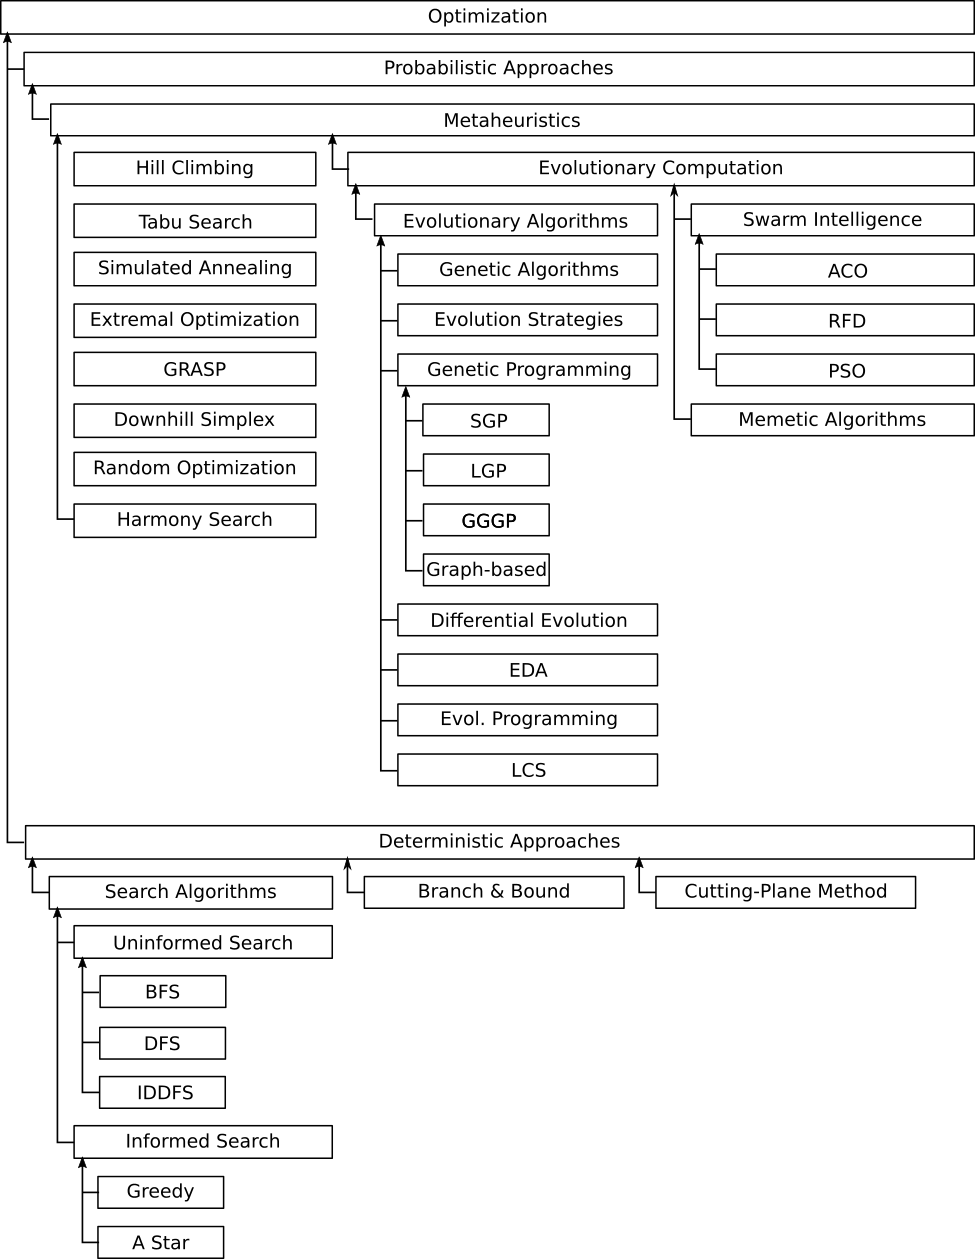
\includegraphics[width=.9\linewidth]{overview_optimisation_algorithm.png}
  \end{sidecaption}
\end{figure}

\subsection{Le domaine des algorithmes métaheuristiques, une sous-discipline de l'Optimisation}

\subsubsection{Q'est ce que l'optimisation ?}
\label{ssec:Optimisation}

Pour \textcite[22]{Weise2011}, l'optimisation \foreignquote{english}{ [...] is the process of solving an optimization problem, i. e., finding suitable solutions for it}, un problème d'optimisation nécessitant de trouver \foreignquote{english}{ [...] an input value $x^*$ for which a mathematical function $f$ takes on the smallest possible value (while usually obeying to some restrictions on the possible values of $x^*$ )}, la notation mathématique astérisque $^*$ désignant ici une valeur optimale.

Sortie de cette définition mathématique, l'optimisation peut également se définir par la mise en oeuvre d'algorithmes spécifiques. La littérature informatique met à disposition des programmeurs un ensemble d'algorithmes capables de fournir des solutions exactes dans un temps fini à un certain nombre de problèmes bien définis. C'est le cas par exemple des nombreux algorithmes de tri. Une autre classe d'algorithmes (\textit{optimization algorithms}) peut être employée lorsqu'il n'existe pas d'algorithme dédié (\textit{dedicated algorithms}), soit parce que le problème est trop spécifique, soit parce que personne n'a trouvé de solution efficace pour résoudre ce problème. 

Dans ce cadre, le terme d'optimisation globale \foreignquote{english}{ [...] is optimization with the goal of finding solutions $x^*$ for a given optimization problem which have the property that no other, better solutions exist.} Le terme \enquote{global} nécessite à la différence d'une recherche qui serait \enquote{locale}, de se concentrer sur l'obtention souvent plus couteuse et plus complexe d'un optimum global, minimum ou maximum, dominant par sa qualité l'ensemble des valeurs recherchées en entrée de la fonction à optimiser.

Bien que souvent beaucoup plus lent, moins précis, et plus consommateurs de ressources que les algorithmes dédiés, ces algorithmes d'optimisations nécessitent aussi beaucoup moins d'informations pour pouvoir être executés : \foreignquote{english}{Most often, these algorithms only need a definition of the structure of possible solutions and a function $f$ which tells measures the quality of a candidate solution. Based on this information, they try to find solutions for which $f$ takes on the best values.} \autocite[24]{Weise2011}

Ces algorithmes s'appuient donc sur différents types de stratégies pour tirer parti du peu d'information obtenue via cette fonction $f$. De nature très diverse, on retient pour séparer une première fois ces stratégies une typologie en deux classes. 

\begin{itemize}[label=\textbullet]
\litem{\textit{Probabilistic Approaches}} Les approches stochastiques désignées dans la fig. \ref{fig:S_OverviewOptimisation} sont capables de trouver un optimum assez rapidement, mais ne peuvent pas en garantir la propriété \enquote{globale}
\litem{\textit{Deterministic Approaches}} Les approches déterministes également désignées dans la fig. \ref{fig:S_OverviewOptimisation} peuvent certes garantir au moins théoriquement l'obtention d'un optimum global, mais s'éxecutent souvent au détriment d'un coût computationnel elevé.
\end{itemize}

Ces deux approches partagent également des difficultés communes, et découvrent leurs limites à des degrés divers en fonction des stratégies mise en oeuvre, dès lors que l'espace de recherche à parcourir devient trop important.

C'est le cas par exemple de l'espace de recherche de toute une sous-catégorie de problèmes \textit{NP-Complet} \Anote{np_complet_def} d'optimisation combinatoire \textit{Combinatorial Optimization Problems} (COP). Ce domaine contient par exemple les problèmes bien connus du voyageur de commerce \textit{Travelling salesman problem} (TSP), ou encore le problème du sac à dos \textit{Knapsack Problem} (KP) \Anote{note_knapsack}. Avec l'augmentation du nombre d'éléments entrant dans la définition de ces problèmes, il devient impossible de passer en revue l'ensemble des combinaisons (solutions possibles). Ce qui a pour conséquence de rendre difficile tout autant la découverte d'un optimum global, que la mesure de qualité de celui-ci, car pour établir cette dernière il nous faudrait logiquement connaitre la solution optimale, or c'est cela même que nous cherchons. 

Cette première typologie recoupe une autre propriété des algorithmes. La littérature informatique qualifie ainsi d'\textit{exacts} les algorithmes dont l'exécution garantit un résultat optimum à coup sûr, d'\textit{approximate algorithms} les algorithmes capables de donner une mesure proche d'un optimum sans pouvoir en garantir la qualité, et d'\textit{approximation algorithms} les algorithmes capables de donner une mesure proche d'un optimum assortie d'une preuve de qualité. Cette dernière classe n'est pas à confondre avec une classe d'algorithmes cherchant à conserver l'optimalité en limitant par diverses stratégies le coût temporel de résolution, mais bien l'inverse, relâcher la contrainte d'optimalité, mais aussi peu que possible. Les \textit{approximations algorithms} sont une donc une sous classe d'\textit{approximate algorithms}, et constituent une branche d'étude à eux seuls, car même dans le cas de problèmes \textit{NP-Complet}, ils offrent dans des dimensions raisonnables et propres à chacun des problèmes une solution sub-optimale d'erreur mesurable et donc potentiellement améliorable, voire comparable, notamment avec les résultats donnés de façon non analytique par d'autre stratégies.
%http://en.wikipedia.org/wiki/Approximation_algorithm#cite_ref-kann92onthe_3-4

On retrouve parfois rangé \enquote{en vrac} dans la classe des \textit{approximate algorithms} la classe des heuristiques et métaheuristiques, deux termes définis plus en détail dans la section suivante.

%On nomme métaheuristique (\textit{metaheuristic}) ce type d'algorithmes s'appuyant sur des heuristiques (\textit{heuristic}).

\subsubsection{Quelle définition peut on donner pour une heuristique (\textit{heuristic}) ? }
\label{ssec:heuristique}

Le terme heuristique \textit{heuristic} vient du Grec \textit{heuriskein} que l'on peut traduire par \foreignquote{english}{to find}, ou \foreignquote{english}{to discover}. D'usage plus large que dans la simple discipline informatique, nous retiendrons ici ce terme seulement sous son sens spécifique contextuel à l'optimisation. Rattaché à la définition d'un problème (\textit{problem dependent}), on définit une heuristique comme une mesure approximative pour définir la qualité d'une solution candidate \autocite[34]{Weise2011}.

%http://stackoverflow.com/questions/9140860/heuristic-function-for-finding-the-path-using-a-star
%http://stackoverflow.com/questions/9140860/heuristic-function-for-finding-the-path-using-a-star
%http://stackoverflow.com/questions/11779589/connection-between-a-star-search-and-integer-programming-extending-a-star
Si on se penche sur la classe d'algorithmes dédiés au problème de recherche du plus court chemin, les heuristiques sont souvent utilisées en appui des algorithmes de parcours de graphe, soit pour converger plus rapidement vers une solution optimale, soit pour justement se libérer de cette contrainte d'optimalité en visant un gain de temps au détriment de la précision. Si on prend par exemple l'algorithme de Djikstra, celui-ci n'utilise pas d'heuristique et garantit que le plus court chemin résultant sera optimal, car tous les chemins possibles entre le point de départ $A$ et le point final $B$ auront été analysés par celui-ci. Il est néanmoins connu comme étant très coûteux d'utilisation dès que le graphe dépasse un certain nombre de noeuds. L'algorithme déterministe $A^*$ s'appuie par contre sur une fonction heuristique $h(n)$ (une estimation du coût minimal reliant le noeud $n$ au noeud final) pour guider l'algorithme dans le processus incrémental de sélection d'un prochain noeud constitutif d'un chemin. En jouant sur cette heuristique, on est ainsi capable de déterminer si l'algorithme doit mettre la priorité sur la vitesse ou la précision, $h(0)$ étant équivalent ici à l'algorithme de Djikstra. Si l'heuristique est bien choisie (on dit ici que l'heuristique est admissible), alors $A^*$ garanti aussi l'optimalité du chemin trouvé, avec à la clef un coût computationnel moindre, car seule une partie des noeuds de l'ensemble du graphe auront été explorés par l'algorithme. Une autre heuristique misant plus sur la vitesse d'exécution pourra définir un chemin cette fois-ci sub-optimal avec un coût computationnel encore plus réduit. Il est à noter ici que l'utilisation d'une heuristique dans un programme n'est pas forcément motivée par la recherche d'un optimum global, mais par le gain de temps. Ainsi, un utilisateur peut très bien avoir les moyens d'obtenir un chemin optimal (Djikstra) sur une petite combinatoire de noeuds, mais peut vouloir prendre un raccourci en utilisant une méthode moins couteuse ($A^*$). Un scénario très souvent mis en avant dans la programmation de jeux sur ordinateur, où l'on cherche régulièrement à gagner du temps, tout en se rapprochant d'un comportement faillible imitant plus un adversaire de type humain.

La forme prise par une heuristique est variable, et peut aller comme vu ci-dessus avec l'exemple $A^*$ d'une simple fonction mathématique de coût intégrée à un algorithme classique de parcours de graphes, à un algorithme beaucoup plus complexe intégrant de multiples prises de décisions pour estimer ce même coût. Dans le livre \textit{Code Complete} de \textcite[12]{McConnell2004}, celui-ci donne un exemple assez parlant pour illustrer la subtile différence qui sépare la description d'un algorithme employé au sens courant pour désigner un algorithme déterministe exact fournissant à coup sûr une solution, et la description d'un algorithme déterministe ou stochastique heuristique (ou appuyé par une heuristique) fournissant seulement un guide pour trouver, éventuellement, une solution.

\foreignquote{english}{Here's an algorithm for driving to someone's house: Take Highway's 167 south to Puyallup. Take the South Hill Mall exit and drive 4.5 miles up the hill. Turn right at the light by the grocery store, and then take the first left. Turn into the driveaway of the large tan house on the left, at 714 North Cedar}

\foreignquote{english}{Here's an heuristic for getting to someone's house: Find the last letter we mailed you. Drive to the town in the return adress. When you get to town, ask someone where our house is. Everyone knows us - someone will be glad to help you. If you can't find anyone, call us from a public phone, and we'll come get you.}

Il faut toutefois éviter de considérer les heuristiques comme appartenant à la seule classe des \textit{approximate algorithms}, car le terme ne se laisse pas facilement enfermer dans une typologie trop simple. En effet de multiples problèmes trouvent une solution exacte jusqu'à un certain niveau de complexification, à partir duquel on fait généralement appel aux heuristiques, soit par un appel à d'autres méthodes intégrant des heuristiques, soit par une intégration d'heuristiques aux méthodes existantes. Ainsi de nombreuses classes d'heuristiques sont utilisées de façon transversale, et apparaissent donc aussi comme composantes manipulées dans la classes des \textit{approximation algorithms}. L'heuristique gloutonne \textit{greedy algorithm} \Anote{greedy_description} apparaît de façon transversale à la fois comme une solution d'approximation pour le \textit{Knapsack Problem} (KP) mais également comme moteur dans le cadre d'algorithmes déterministes exacts comme la recherche du plus court chemin de Djikstra. Un autre algorithme nommé \textit{A*} (\textit{A-Star}) qui englobe Djikstra comme cas particulier, est quant à lui capable de fournir tout à la fois une mesure exacte ou approximée en fonction de l'heuristique injectée et du niveau de complexité du problème abordé. 

\subsubsection{Quelle définition peut on donner pour une métaheuristique (\textit{metaheuristic}) ?}
\label{ssec:metaheuristique}

Le terme métaheuristique est d'origine plus moderne \autocite{Glover1986}, et a permis d'englober a posteriori des algorithmes jusque là qualifiés d'heuristiques. C'est le cas par exemple d'une bonne partie des algorithmes évolutionnaires, qui émergent principalement au cours des années 1960-1970. Cette remarque d'ordre historique est à l'origine d'une première ambiguité entre les termes auquelle il faut encore ajouter les inquiétudes exprimées par \textcite{Luke2013}. Pour ce dernier, le terme métaheuristique est en réalité plutôt malheureux pour définir cette catégorie d'algorithmes, car contrairement à ce que laisse entendre ce terme, \textit{une heuristique pour ou à propos d'une heuristique}, ce n'est pas de cela dont il s'agit ici.

Voici comment \textcite[8]{Brownlee2012} perçoit la différence entre les deux termes : \foreignquote{english}{Like heuristics, metaheuristics may be considered a general algorithmic framework that can be applied to different optimization problems with relative few modifications to adapt them to a specific problem. The difference is that metaheuristics are intended to extend the capabilities of heuristics by combining one or more heuristic methods (referred to as procedures) using a higher-level strategy (hence ‘meta’). A procedure in a metaheuristic is considered black-box in that little (if any) prior knowledge is known about it by the metaheuristic, and as such it may be replaced with a different procedure. Procedures may be as simple as the manipulation of a representation, or as complex as another complete metaheuristic. Some examples of metaheuristics include iterated local search, tabu search, the genetic algorithm, ant colony optimization, and simulated annealing.}

Le terme \enquote{méta-} renvoie plus en définitive au concept générique de \enquote{stratégie de recherche} prenant la forme d'un algorithme d'optimisation capable de mélanger, manipuler des heuristiques ou d'autres métaheuristiques (cf. points \ref{enum_meta_a} et \ref{enum_meta_h}) \Anote{def_meta_weise}. Contrairement aux heuristiques, les métaheuristiques se définissent plus comme un système fait de composants, dont la plasticité permet le support et l'interaction nécessaire au développement d'heuristiques plus ciblées (\textit{problem dependent}) \Anote{def_meta_sorensen}. La structure offre un patron d'usage initial (\textit{pattern}) qui reste indépendant du problème abordé (\textit{problem independent}) (cf. \ref{enum_meta_g}), tout en restant évolutif, comme le montre le fort développement de cette discipline depuis les années 1980. Ce principe de flexibilité, on le retrouve par exemple dans la classe des EC, comme le mettent bien en valeur Bach, Hammel et Schwefel en 1997, dans une publication introduisant l'EC dans la série renommée des \textit{IEEE Transactions} :

\foreignquote{english}{We argue that the most significant advantage of using evolutionary search lies in the gain of exibility and adaptability to the task at hand, in combination with robust performance (although this depends on the problem class) and global search characteristics. In fact, evolutionary computation should be understood as a general adaptable concept for problem solving, especially well suited for solving difficult optimization problems, rather than a collection of related and ready-to-use algorithms. The majority of current implementations of evolutionary algorithms descend from three strongly related but independently developed approaches: genetic algorithms,evolutionary programming , and evolution strategies. [...] The fundamental difference in the evolutionary computation approach is to adapt the method to the problem at hand. In our opinion, evolutionary algorithms should not be considered as off-the-peg, ready-to-use algorithms but rather as a general concept which can be tailored to most of the real-world applications that often are beyond solution by means of traditional methods. Once a successful EC-framework has been developed it can be incrementally adapted to the problem under consideration, to changes of the requirements of the project, to modifications of the model and to the change of hardware resources.} \autocite{Back1997a}

Enfin, toujours dans une tentative de positionner ce terme dans une typologie, il faut savoir qu'une classification trop rapide de ces méthodes dans les seuls \textit{approximate algorithms} peut également être critiqué. Si les méthodes métaheuristiques sont effectivement souvent connues pour ne pas avancer de preuve, des travaux récents montrent toutefois qu'il existe de nouveaux algorithmes permettant de garantir dans certaines conditions un optimum global (CP-Algorithm de \autocite{Reuillon2015}). Tout dépend donc du degré et de la nature que l'on veut bien associer à la notion d'\textit{approximation} lorsqu'il s'agit de fournir une mesure d'éloignement de l'optimum. Les \textit{approximation algorithms} semblent toutefois plus intéressés par l'établissement d'une preuve au sens mathématique, et se concentrent avant tout sur un ensemble relativement limité de problèmes d'optimisation discret, ce qui ne semble pas être le but des métaheuristiques dans les deux cas. \autocites[1-6]{Kann1992}[13-15]{Williamson2011} %Metaheuristics: From Design to Implementation Par El-Ghazali Talbi

%You could think of a heuristic like an approximate (not approximation) solution to a problem. The difference between approximate and approximation is that the first is about getting a good guess of the solution of a problem, but that you don't really know how good it is. The second is about getting a solution for which you can prove how close it is to the optimal solution.

Enfin bien d'autres sous classifications sont possibles prenant plus ou moins en compte les spécificités propres aux différents algorithmes, comme celle opposant par exemple les stratégies utilisées en interne pour parcourir l'espace de recherche (generationel contre \textit{steady-state}, ou individuel contre populationel), la dimensionnalité possible pour la résolution des problèmes (mono-objectif contre multi-objectif), l'inspiration d'origine (naturelle biologique contre inspirations autres), etc. 

Toute classification monocritère est donc rendue très difficile, une voie s'étant même ouverte pour tenter de classer ces algorithmes suivant la nature et le niveau d'opération de ces hybridations. L'origine de cette difficulté tient dans une pratique courante et assumée d'hybridation entre les différentes techniques afin de réunir le meilleur de chacune d'elles au sein de nouvelle proposition de recherche. De fait, il est important pour la suite de cerner au mieux la classe d'algorithme d'optimisation que nous allons aborder, et de définir pourquoi nous l'avons abordé. Nous nous intéresserons principalement dans la suite de cette présentation aux approches stochastiques métaheuristiques inspirées par la métaphore biologique, nommée \textit{Evolutionary Computation} (EC) ( voir figure \ref{fig:S_OverviewOptimisation}). La section \ref{xx} permettra de dégager les spécificités de cette subdivision, mais en attendant il nous faut d'abord présenter les principaux termes et concepts communs à cette classe d'algorithmes d'optimisation. 

Devant la difficulté d'établissement d'une définition englobante, plusieurs auteurs semblent s'accorder pour faire du rattachement d'un algorithme à cette catégorie, une correspondance plus ou moins lâche avec un ensemble de propriétés généralement observées. En évitant une définition trop vague ou trop restrictive, on espère ainsi récupérer dans cette classe certains hybrides intéressants. 

Voici un exemple de propriétés issues de \textcite{Blum2003} et traduites ci dessous :

%label=$\blacktriangleright$
\begin{enumerate}[label=(\alph*),labelindent=\parindent,leftmargin=*]
	\item Les métaheuristiques sont des stratégies qui \enquote{guident} le processus de recherche. \label{enum_meta_a}
	\item Leur objectif est d'explorer l'espace de recherche efficacement pour trouver les solutions quasi-optimales. \label{enum_meta_b}
	\item L'étendue des techniques que constitue la classe des algorithmes métaheuristiques va de la simple recherche locale à un processus d'apprentissage complexe. \label{enum_meta_c}
	\item Les algorithmes métaheuristiques sont approximatifs et la plupart du temps non déterministes. \label{enum_meta_d}
	\item Les métaheuristiques peuvent incorporer des mécanismes pour éviter d'être piégé dans une portion confinée de l'espace de recherche. \label{enum_meta_e}
	\item Les concepts de bases des métaheuristiques permettent d'adopter un certain degré d'abstraction dans la description. \label{enum_meta_f}
	\item Les métaheuristiques ne sont pas \textit{problem-specific}. \label{enum_meta_g}
	\item Les métaheuristiques peuvent faire usage d'une expertise du domaine au travers des heuristiques controlées par une stratégie de plus haut niveau. \label{enum_meta_h}
	\item La plupart des métaheuristiques actuelles font appel à une mémoire pour améliorer le processus qui guide la recherche. \label{enum_meta_i}
\end{enumerate}

Afin de mieux comprendre cette table de propriétés un peu abstraite, il est proposé de reprendre ces différents points au travers d'une lecture commentée, en commencant par une question ciblé sur la mécanique interne régissant ce type de technique.

\textit{Comment se matérialise la recherche de solutions optimisées dans une métaheuristique ?}

Si on considère les problèmes de combinatoires discrets comme \textit{TSP} ou \textit{Knapsack}, on a déjà vu que le nombre de combinaisons à évaluer lors d'une augmentation du nombre d'éléments participant à la définition du problème devient très vite problématique si on cherche à trouver une solution optimale exacte. Si on prend le cas d'un exemple plus ludique d'optimisations discrètes dans la branche des jeux (\textit{Combinatorial game theory}), le nombre de combinaisons légales possibles pour un plateau de 19 par 19 dans le jeu de GO chinois est estimé par \textcite{Tromp2007} à $2.08168199382×10^{170}$ . Même si certains auteurs comme Tromp estime qu'un tel calcul sera possible d'ici quelques années, les problématiques posés par ce jeu mettent au défi les meilleurs programmes en intelligence artificielle \autocite{Bouzi2001}, et cela malgré des progrès spectaculaires ces dernières années, via notamment l'utilisation d'heuristique plus efficace que les approches classiques \Anote{mcts_go}.  Dans le cas d'un problème continu discrétisé, comme la recherche des meilleures valeurs de paramètres pour une simulation, la mise en oeuvre d'un plan factoriel complet (d'autres types de stratégies beaucoup plus fines existent) pose un problème double. 

\hl{Correction orthographe à faire}
D'une part ce choix ne résout en rien la problématique combinatoire. Donnons un exemple plus concret, si une simulation possède 5 paramètres, chacun de ces paramètres étant discrétisé en 10 pas, cela nous donne déjà $10^5$ combinaisons possibles à évaluer. Si on considère que le modèle de simulation ainsi exécuté est stochastique (10 réplications), dans un délai relativement rapide (1 minute), la durée totale d'exécution de ce plan, pourtant relativement \enquote{grossier} d'un point de vue de la couverture de l'espace des paramètres, est environ égale à 2 années de calcul... La parallélisation d'un tel calcul, c'est à dire son execution sur plusieurs processeurs ou ordinateurs en parallèle, pourrait évidemment réduire ce temps de calcul à des dimensions plus raisonnables, mais c'est sans compter sur un deuxième problème, plus contraignant.

Avec le choix d'une telle maille pour la discrétisation des paramètres, c'est prendre le risque de passer à côté de solutions potentielles, une problématique contraignante d'autant plus qu'elle se complexifie avec l'augmentation du nombre de paramètres, comme le dicte le phénomène de \textit{Curse Dimensionality} établit par Richard Bellman. Ce problème est principalement d'ordre statistique, là ou 100 points peuvent suffire dans un espace entre $(0..1)$ de dimension $1$ pour commencer à inférer ($0.01$ de distance entre chaque point), 100 points dans un même espace $(0..1)$ de dimension $10$ ne couvre plus qu'une toute petite partie du volume disponible. Chaque point est alors entouré d'une large portion de vide qui rend délicates toutes inférences à partir d'une si faible couverture d'un tel espace. Pour obtenir une couverture équivalente avec une distance de $0.01$ entre chaque points, il faudrait disposer de $10^{20}$ points, ce qui semble considérable \autocite{Bellman1961}.

Contrairement à d'autres méthodes d'optimisations, les métaheuristiques font généralement appel à un processus d'échantillonnage (voir point \ref{enum_meta_b}) pour explorer de façon stochastique un espace de recherche de toute façon beaucoup trop vaste pour être parcouru de façon exhaustive. Cela permet de repousser en partie ce problème de couverture de l'espace de paramètres lié à l'augmentation de la dimensionnalité du problème, cas nous verrons que les méta-heuristique opérant dans des espace de paramètres discret mais aussi continu, sans qu'une discrétisation préalable soit nécessaire en amont.

C'est pour cela que \textcite[7]{Luke2013} nous propose de voir ce type de problème autrement, partant du postulat assez logique qu'une solution \enquote{même non optimale} est un point de départ pour l'amélioration de toute façon bien meilleure que \enquote{pas de solution du tout}.

\foreignquote{english}{ Metaheuristics are applied to \enquote{I know it when I see it} problems. They're algorithms used to find answers to problems when you have very little to help you: you don't know what the optimal solution looks like, you don't know how to go about finding it in a principled way, you have very little heuristic information to go on, and brute-force search is out of the question because the space is too large. But if you're given a candidate solution to your problem, you can test it and assess how good it is. That is, you know a good one when you see it.}  

\hl{schéma}

Suivant ce raisonnement, la connaissance d'un problème se construit au travers d'une confrontation répétée de nos représentations, de nos interrogations avec la forme réelle et encore inconnue prise par celui-ci. La carte de ce nouveau territoire se révélant peu à peu dans la projection sur l'espace des solutions des choix effectués lors de la sélection des nouveaux candidats à évaluer (solutions candidates).

Les métaheuristiques sont donc là pour faciliter l'exécution de cette tâche complexe et répétitive qui consisterait à améliorer notre connaissance du problème en proposant de façon pertinente de nouvelles solutions candidates à évaluer, ces dernières étant choisies si possible en fonction des résultats obtenus par les précédentes (voir point \ref{enum_meta_i}). La perspective d'une telle automatisation pose évidemment un certain nombre de questions. 

Quels sont les choix mis à disposition de l'optimiseur pour améliorer la réponse attendue des solutions candidates entre chaque incrément ? \autocite[19]{Weise2011} 

Une comparaison automatisée nécessite pour être mise en oeuvre de définir \begin{enumerate*}[label=(\alph*)]
\item sur quelle base se fonde l'évaluation d'une solution,
\item la comparaison entre les solutions évaluées, 
\item et la sélection de nouvelles solutions candidates.\end{enumerate*} Car l'optimiseur, tout comme nous, ne connait pas directement la forme prise par l'espace des solutions, et doit bien concevoir en interne les choix permettant, par la selection de nouvelles solutions candidates à évaluer, de progresser si possible vers une solution optimum.

De fait dans un tel scénario, et pour éviter une recherche aléatoire, l'évaluation de solution candidate renvoie à l'existence d'une expertise externe à l'optimiseur, le seul capable de formaliser ce qui différencie une bonne solution d'une mauvaise solution. On revient à parler ici d'heuristique, et de leurs diversités, car si celles-ci interviennent dans l'évaluation des solutions candidates (a), elles interviennent aussi dans les autres cas (b) et (c). Elles se présentent sous la forme de différents types de connaissances, interrogent différents espaces, et s'intègrent souvent sous la forme de composants dans la structure plastique des métaheuristiques.

L'injection de connaissance (voir point \ref{enum_meta_h} )dans ce type d'algorithme métaheuristique est donc double, et opère à la fois de façon précise dans la formalisation d'un ou de plusieurs critères qui vont servir pour l'algorithme optimiseur à déterminer la qualité, bonne ou mauvaise, d'une solution candidate; et de l'autre elle intervient cette fois ci de façon moins contrôlable dans la façon dont l'expérimentateur va construire et paramétrer une métaheuristique pour l'adapter au mieux à son problème. La qualité interne (paramètre, structure) de la métaheuristique définit aussi en quelque sorte le processus d'exploration, ce qui explique aussi la dépendance de ce type d'algorithmes à l'environnement qu'ils doivent explorer.

\begin{figure}[ht]
	\begin{sidecaption}[fortoc]{Projection du vecteur de points $\{a \dotsc n\}$ dans l'espace des objectifs. Les couleurs représentent les différents axes de projection ordonnés de 1 à 3 sur $(x,v)$ et de 1 à 4 sur $(y,v)$}[fig:spacePspaceOmultimodal]
	 \centering
	 	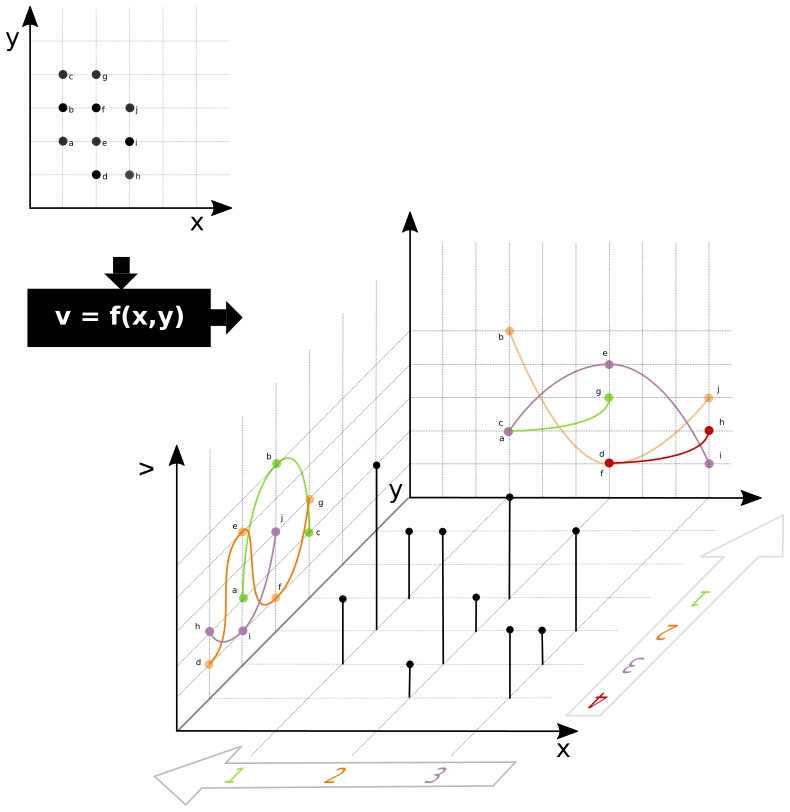
\includegraphics[width=.9\linewidth]{espaceP_espaceO_multimodal.pdf}
	\end{sidecaption}
\end{figure}

L'objectif est rendu complexe car la relation entretenue entre ces deux espaces, celui des solutions candidates disponibles, et celui des évaluations est bien souvent dissymétrique. Pour mieux comprendre cette relation, la figure \ref{fig:spacePspaceOmultimodal} illustre cette correspondance des solutions candidates $\{a \dotsc n\}$ décrites par leurs coordonnées $(x,y)$ lorsqu'elles sont projetées dans l'espace des objectifs $\mathbb{Y}$ en suivant la transformation attendue par la fonction boite noire de dynamique non linéaire $f(x,y)$. Les valeurs $v = f(x,y)$ des différentes solutions candidates sont également projetées sur le plan 2D $(x,v)$ et $(y,v)$ pour mieux visualiser la forme prise par cette surface en 2D.

\begin{figure}[!htbp]
	\begin{sidecaption}[fortoc]{Les couleurs indiquent la  des valeurs $v = f(x,y)$ mesurée dans la figure \ref{fig:spacePspaceOmultimodal}, sachant qu'on cherche à minimiser la valeur de v :
\parbox{\marginparwidth}{
\begin{enumerate}[label={},labelindent=0pt,leftmargin=*]
        \item \sqbox{tangoBlue1} indique une fitness minimale, cf. qui maximise $v$
        \item \sqbox{tangoOrange1} indique une fitness intermédiaire et,
        \item \sqbox{tangoRed1} indique une fitness maximale, cf. qui minimise $v$
\end{enumerate}}}[fig:xyspacePspaceOmultimodal]
	 \centering
	  \subbottom[]{
	 	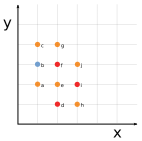
\includegraphics[width=0.4\linewidth]{xyespaceSolutionCandidate_a.pdf}
	 	\label{subfig_xyespaceSolutionCandidate_a}}
	 \subbottom[]{
	 	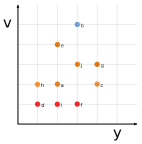
\includegraphics[width=.4\linewidth]{xyespaceSolutionCandidate_b.pdf}
	 	\label{subfig_xyespaceSolutionCandidate_b}}
	 \subbottom[]{
		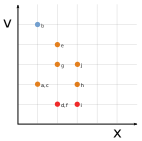
\includegraphics[width=.4\linewidth]{xyespaceSolutionCandidate_c.pdf}
		\label{subfig_xyespaceSolutionCandidate_c}}
	\end{sidecaption}
\end{figure}

Pour visualiser la valeur $v$ prise par chacune des solutions candidates, on projette celle-ci dans l'espace $(x,y)$, ce qui nous permet de mieux constater l'éclatement des valeurs de $v$ sur la figure \ref{fig:xyspacePspaceOmultimodal}.

Deux solutions proches dans l'espace des solutions candidates peuvent amener à des résultats très différents, et inversement, pour deux évaluations proches peuvent correspondre des solutions candidates très éloignées, comme le détaille la figure \ref{fig:xytrajectoire}. Il s'agit d'une propriété bien connue des fonctions non linéaires, qu'elles soient décrites de façon explicite via le formalisme mathématique, ou de façon implicite dans l'expression des dynamiques complexes de modèles de simulation.

Il est clair que l'information récoltée par un tel déplacement basé sur une distance euclidienne dans le plan $(x,y)$ n'est pas vraiment pourvoyeur d'intuitions sur l'emplacement possible des meilleures solutions (voir figure \ref{fig:xytrajectoire}). Il semble par exemple plus intéressant pour l'optimiseur d'accéder aux solutions par le prisme d'ensembles construits sur la base d'une valeur $v$ commune (voir figure \ref{fig:xyspacePspaceOmultimodal}). Une information qui peut être exploitée de multiples façons, toujours en permettant à l'optimiseur de déterminer un nouvel ensemble de solutions candidates à évaluer.

\begin{figure}[!htbp]
	\begin{sidecaption}[fortoc]{Représentation de deux déplacements dans l'espace des solutions candidates et son équivalent dans l'espace des objectifs
	\parbox{\marginparwidth}{
	\begin{enumerate}[label=(\alph*),labelindent=\parindent,leftmargin=*]
	        \item Partant de $b$, on se déplace d'une unité vers $c$ ou $a$, ce qui dans l'espace des objectifs équivaut également à un déplacement vers $h$; $v=2$ pour $v_h, v_a, v_c$
	        \item Partant de $b$, on se déplace toujours d'une unité vers $f$, ce qui dans l'espace des objectifs équivaut également à un déplacement vers $d$ et $i$; $v=1$ pour $v_d,v_i,v_f$
	\end{enumerate}}}[fig:xytrajectoire]
	 \centering
	  \subbottom[]{
	 	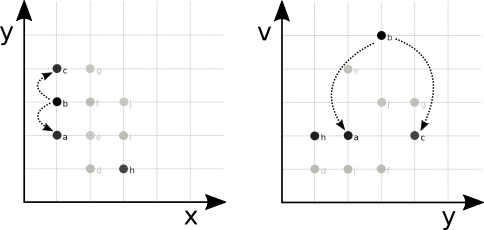
\includegraphics[width=0.6\linewidth]{xytrajectoire_a.pdf}
	 	\label{subfig_xytrajectoire_a}}\qquad
	 \subbottom[]{
	 	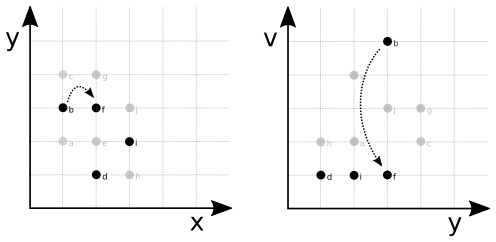
\includegraphics[width=.6\linewidth]{xytrajectoire_b.pdf}
	 	\label{subfig_xytrajectoire_b}}
	\end{sidecaption}
\end{figure}

Si l'obtention d'une cartographie complète d'un tel espace de solutions peut être l'objectif de ce type de raisonnement, la recherche d'un optimum en est un autre. Dans un cas on aura tendance à maximiser la diversité dans le choix de solutions candidates à évaluer, afin d'essayer de couvrir au mieux le territoire à explorer. Cette idée on la retrouve dans l'établissement d'une \textit{fitness landscape}, ou dans sa version multi-objectif, d'un \textit{problem landscape} \autocite[93-94]{Weise2011}, un paysage cumulé de l'espace des objectifs indiquant toutes les valeurs prises par ceux-ci au cours de l'exploration \Anote{paysage_cumule}. Un espace mis à profit par l'optimiseur pour améliorer la proposition de solution candidate, par exemple en se basant sur la construction de cluster de valeurs intéressantes comme indiqué précédemment, ou encore en cherchant à favoriser les zones de cet espace encore peu explorées, etc. Alors que dans le cas d'une optimisation pour la calibration ou la prédiction, trouver le plus rapidement possible un minimum local ou global peut constituer un objectif suffisant.

En réalité, ces deux objectifs sont souvent liés, et c'est souvent l'expertise humaine intervenant de façon externe à l'optimiseur qui va déterminer l'importance de l'un ou de l'autre dans la stratégie à suivre. Dans le cas par exemple d'une optimisation de paramètres nécessaire à la marche efficiente d'une centrale nucléaire, la découverte d'un minimum local robuste peut s'avérer beaucoup plus intéressante qu'un minimum global instable. La topologie proche de l'espace des solutions déjà exploré peut constituer un facteur de connaissance d'intervention plus ou moins importante dans l'expertise d'une bonne ou d'une mauvaise solution. 

Cette mécanique on la retrouve également à un autre niveau, dans le fonctionnement interne des métaheuristiques. En effet, celles-ci s'appuient le plus souvent sur la métaphore biologique évolutive pour mettre en tension une recherche de solutions guidée toute à la fois par l'\textit{exploration} (trouver des solutions originales), et l'\textit{exploitation} (améliorer les solutions existantes). 

\begin{figure}[!htbp]
\begin{sidecaption}[fortoc]{Recherche d'un minimum global.}[fig:hmap2ab]
 \centering
 \subbottom[Une fonction $f(x)$ présentant un unique minimum global]{
 	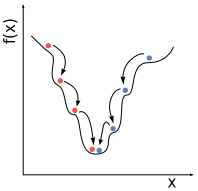
\includegraphics[width=.4\linewidth]{heightmap2a.pdf}
 	\label{subfig_hmap2ab_a}}\qquad
 \subbottom[Une fonction $f(x)$ présentant un minimum local et global]{
	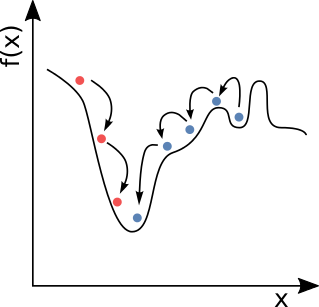
\includegraphics[width=.4\linewidth]{heightmap2b.pdf}
	\label{subfig_hmap2ab_b}}
\end{sidecaption}
\end{figure}

Les opérateurs intervenant comme stratégies dans la médiation de ces deux concepts sont conçus pour éviter à l'optimiseur un certain nombre d'écueils. Trop longue pour être abordée ici de façon exhaustive, cette liste évoquant les problèmes et solutions qui résultent du rapport entre les formes de problèmes abordés et les faiblesses génériques ou dépendantes des métaheuristiques utilisées, \textcite{Weise2011} en donne une description experte sur une centaine de pages. On peut également se référer à une autre synthèse, abordant ces problèmes avec un angle un peu plus spécifique aux algorithmes évolutionnaires, réalisée en 2001 par \textcite[316-445]{Deb2001}.

En se limitant aux pièges dépendant de la topologie de l'espace des solutions (voir point \ref{enum_meta_e}), \textcite[140]{Weise2011} a proposé un tableau synthétique dont on extrait ici quelques exemples légèrement modifiés pour éclairer notre argumentaire. Les exemples des figures \ref{fig:hmap2ab} et \ref{fig:hmap2cd} mettent en oeuvre un optimiseur générant de façon incrémentale de nouvelles solutions, chacune représentée par un point. Il faut donc lire ces exemples en tenant compte du fait qu'ils présentent une représentation cumulative des différents points parcourus dans le temps par l'optimiseur.

La figure \ref{fig:hmap2ab} démontre un fonctionnement normal de l'optimiseur, capable quelque soit son placement initial (rouge ou bleu), de trouver le minimum global d'une fonction relativement simple \ref{subfig_hmap2ab_a}. Un comportement équivalent est observable dans la figure \ref{subfig_hmap2ab_b}, le compromis \enquote{exploitation - exploration} étant suffisant pour que l'optimiseur bleu surmonte l'obstacle posé par la présence d'un minimum local dans cette fonction.

\begin{figure}[!htbp]
  \begin{sidecaption}[fortoc]{Deux types de fonctions sont rendues difficiles à optimiser du fait d'une topologie marquée.}[fig:hmap2cd]
  \centering
  \subbottom[Une fonction $f(x)$ multimodale acceptant plusieurs minimum locaux, et un seul minimum global]{
  	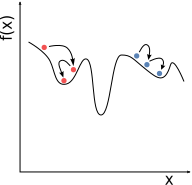
\includegraphics[width=.4\linewidth]{heightmap2e.pdf}
  	\label{subfig_hmap2cd_c}}\qquad
  \subbottom[Une fonction $f(x)$ contenant très peu d'information de gradient pour guider l'optimiseur]{
	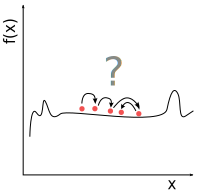
\includegraphics[width=.4\linewidth]{heightmap2c.pdf}
  	\label{subfig_hmap2cd_d}}
 \end{sidecaption}
\end{figure}

A l'inverse, on perçoit bien sur ce schéma \ref{subfig_hmap2cd_c} quel effet peut avoir un déséquilibre entre les deux stratégies, une exploitation trop appuyée au détriment de l'exploration amenant souvent à une convergence \Anote{def_convergence} prématurée, c'est-à-dire à un piège dans un optimum local. 

La figure \ref{subfig_hmap2cd_d} montre également que face à une topologie de fonction présentant un plateau relativement uniforme, l'optimiseur sera en peine pour trouver un minimum, même local. Un paramétrage différent de l'exploration pourra peut être résoudre ce problème, sans pour autant que l'on en soit sur. 

Ce qui nous permet d'évoquer une faiblesse connue des métaheuristiques, héritée des remarques déjà faites sur les algorithmes d'optimisations stochastique \Anote{stochastic_note} dans laquelle on les place habituellement. La découverte garantie d'une solution globale optimale est en général difficile avec ce type d'algorithmes (voir point \ref{enum_meta_d}) \Anote{equipe_mixite}, au moins pour deux raisons : 

\begin{enumerate}
\item la variabilité qui opère lors de la selection des solutions candidates à un instant $t$ ne permet pas de garantir qu'il n'existe pas quelque part une solution candidate sélectionnée à $t+1$ dont l'évaluation révélera un meilleur optimum. La définition d'un critère d'arrêt est donc rendue délicate.
\item La variabilité dans l'établissement d'une trajectoire de recherche implique qu'un algorithme de même qualité puisse passer une première fois à coté d'un optimum, et une deuxième fois trouver celui-ci. 
\end{enumerate}

\begin{figure}[!htbp]
\begin{sidecaption}[fortoc]{Représentation d'une navigation indirecte de l'optimiseur dans un espace de solution $z = f(x,y)$.}[fig:hmap1]
  \centering
  \subbottom[]{
  	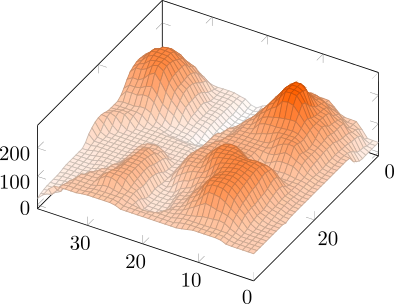
\includegraphics[width=.4\linewidth]{heightmap1a.png}
  	\label{subfig_hmap_a}}\qquad
  \subbottom[]{
	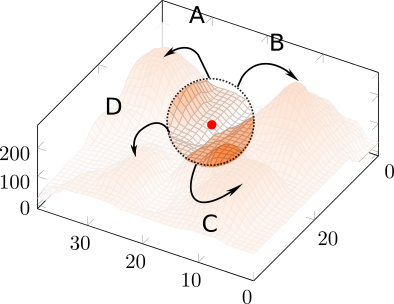
\includegraphics[width=.4\linewidth]{heightmap1b.png}
  	\label{subfig_hmap_b}}
\end{sidecaption}
\end{figure}

Pour mieux comprendre les problèmes posés par des espaces de solutions multi-modaux, déjà figurés en deux dimensions dans \ref{subfig_hmap2cd_c}, on représente cette fois ci dans la figure \ref{fig:hmap1} l'optimiseur dans un espace en trois dimensions similaire à celui vu dans la figure \ref{fig:spacePspaceOmultimodal}, à la recherche d'un optimum global. La fonction ainsi représentée comporte deux entrées $(x,y)$, et une sortie $z = f(x,y)$ représentant la valeur numérique résultat de l'optimisation.

Attention à la lecture de ces schémas, il ne faut pas oublier que l'optimiseur \textbf{ne se déplace pas directement} sur le terrain visible dans la figure \ref{subfig_hmap_a}, et pour laquelle celui-ci n'a justement aucune visibilité. C'est un peu comme visualiser un labyrinthe de l'extérieur sur une feuille, puis de l'intérieur quand on s'y projette, la difficulté pour résoudre celui-ci n'est plus la même. La visibilité dont dispose l'optimiseur est celle des résultats de solutions candidates déjà évaluées (voir point \ref{enum_meta_i}). Il s'agit donc de proposer de nouvelles solutions candidates soit en les composant à partir d'une manipulation des solutions candidates déjà évaluées, soit en introduisant de toutes nouvelles solutions candidates prises de façon aléatoire. Au cours de l'itération mesurant la progression de l'algorithme, c'est bien l'évaluation de cette nouvelle population de solutions candidates qui détermine si il y'a effectivement eu un déplacement qualitatif dans l'espace des solutions evaluées. Le déplacement du point rouge dans cet espace n'est donc effectif que si on trouve à un instant $t + 1$ une solution plus intéressante qu'à l'instant $t$.

A partir des résultats de la première solution candidate évaluée figurée ici en rouge dans \ref{fig:hmap1}, les opérateurs de recherches soumis à l'aléa d'une recomposition ou d'un tirage aléatoire peuvent tout à fait proposer un candidat à $(x,y)_{t+1}$ qui débouche sur un résultat $z = f(x,y)$ plaçant l'optimiseur dans le sillon d'un gradient de pente parmi plusieurs. Ce qui mènera probablement l'optimiseur à découvrir des optimums de qualités très différentes : $A$ (local), $B$ (global), $C$ (local), $D$ (local). 

Autrement dit, en plus de la stochasticité inhérente de ces algorithmes, non seulement un algorithme de type $A$ n'aura pas les mêmes résultats qu'un algorithme de type $B$, mais celui-ci sera également différent d'un algorithme $A'$ du fait d'un paramétrage différent.

Comme déjà évoqué dans les différentes définitions, on retrouve ici la qualité de flexibilité des métaheuristiques, permettant de transformer ce qui pourrait de prime abord paraitre pour un défaut, en qualité. L'utilisation de celle-ci permettant d'étendre toujours un peu plus leurs champs d'utilisation, en facilitant la réponse aux questions suivantes \Anote{q_ppr} : 
\begin{enumerate}
\item  \foreignquote{english}{What parameter settings do I use to get good results when applying heuristic method X to problem Y?}
\item  \foreignquote{english}{How do I adjust the parameters of heuristic X so I get better results on problem Y?}
\item \foreignquote{english}{Which is \enquote{better}, heuristic X or heuristic Y?}
\end{enumerate}

On pourrait ainsi ne retenir que cette citation de source inconnue, lorsqu'elle définit une métaheuristique comme \foreignquote{english}{ a pretty good rule for finding pretty good rules.}

Cette flexibilité vient compléter et compenser efficacement cet horizon de connaissance assez limité, nécessaire à une généricité d'emploi. Les métaheuristiques fournissent ainsi le support générique initial pour en faire un outil d'usage indépendant du problème, tout en fournissant les outils pour favoriser également leur propre modification en vue d'une amélioration de résultat pour un problème donné. Elle cumule donc en quelques sortes les deux propriétés de dépendance et d'indépendance face à un problème donné. 

De plus, la recherche dans cette discipline ne se contente pas d'organiser une forme de compétition qui mènerait à elle seule, par l'apprentissage répété de fonctions aussi standardisées que celles utilisées dans les figures précédentes, à une surestimation de certains algorithmes \Anote{test_fonction_surutilisation}, et se nourrit également d'une recherche plus appliquée à des problématiques réelles. Ce qui permet par effet retour, d'espérer voir appliquer à des formes de problèmes génériques, des opérateurs dédiés à l'origine à des problématiques spécifiques. La construction et l'évaluation d'heuristique plus performante servant toujours indirectement une cause plus générale.

Enfin, une des propriétés qui n'a pas encore été introduite dans ce résumé est la capacité de notation et de description abstraite des métaheuristiques (voir point \ref{enum_meta_f} ). Des concepts de plus haut niveau sont introduits pour désigner l'expression et la manipulation d'heuristiques et de classes d'heuristiques dans un système composant la métaheuristique. Mais avant de pouvoir introduire ces subtilités de typologie propre à chaque classe de métaheuristique, il faut également rappeler l'existence d'une base commune de formalisation mathématique permettant la description des problèmes. Autrement dit, cela revient à introduire ou à poser sur une partie des mots déjà utilisés dans cette section, un certain nombre de notations mathématiques d'utilisation relativement standard dans cette communauté informatique utilisant les métaheuristiques.

Il nous restera également à aborder dans la section suivante, la question des \textbf{moyens} mis à disposition de l'optimiseur pour opérer la selection de nouveaux candidats à évaluer. Jusqu'ici seule une représentation de ces solutions candidates dans l'espace des solutions candidates possibles a été abordée, ainsi que l'espace contenant les résultats des solutions candidates évaluées. Mais ces deux espaces ne constituent pas les véritables espaces sur lesquels l'optimiseur est amené à travailler, et cela bien qu'il puisse les intégrer à son expertise pour la selection de nouveaux candidats à l'évaluation \Anote{remarque_section_metaheuristique}. 

\hl{les 4 paragraphe ci dessous sont à faire descendre avec notation mathématique, pour compléter la section suivante, et sans briser le suspens ?}

L'introduction d'un nouvel \enquote{espace de recherche} est nécessaire, et  correspond à la somme des entrées, des paramètres, sur lequel l'optimiseur va pouvoir jouer directement, afin de modifier cette fois-ci indirectement l'expression de la solution candidate ensuite évaluée.

Autrement dit, il faut retenir qu'une solution candidate fait partie d'un espace de solutions candidates possibles, et que l'exploration de ce dernier est dépendant des bornes fixées par l'expert pour délimiter l'espace de recherche de chacun des entrant, notamment pour limiter le champ de recherche de l'optimiseur à celui des valeurs empiriquement et théoriquement possibles. Ce qui introduit aussi la possibilité d'une nouveau \textit{mapping} entre les valeurs de ces deux espaces, de recherche, et du phénomène à évaluer, qui ne sont pas nécessairement de même nature. 

On peut s'appuyer sur l'exemple de bras robotisé donné par \autocite{Weise2011} pour illustrer ce cas. On a d'un côté les paramètres de positionnement des éléments de bras d'un robot, contraint par la structure théorique de celui-ci, et de l'autre l'expression spatiale finale du bras représentatif de cette combinaison de paramètres dans l'espace des solutions possibles, potentiellement infini, et dont on n'a pas la maitrise directe. L'optimiseur s'appuie ensuite sur l'évaluation de cette configuration spatiale à l'aide des critères qu'on lui a donné pour induire des opérations non pas dans l'espace d'expression spatialisé du bras, mais dans l'espace de recherche des vecteurs de paramètres permettant l'amélioration de ce résultat.

\subsubsection{Une formulation mathématique standardisée pour encadrer les problèmes d'optimisations et les métaheuristiques}
\label{ssec:math_opti}

%search space p 82
%structure p 101
% pareto ranking p 275
																								
Pour comprendre comment se déroule de façon générale la résolution d'un problème d'optimisation, il faut poser un certain nombre de notions qui nous seront utiles par la suite. Cet exercice de description plus mathématique et générique s'appuie là encore principalement sur les écrits de \textcite{Weise2011}

La première étape selon Weise dans la construction d'un problème d'optimisation est de définir le type de structure qui peut être associée à l'expression des solutions possibles et spécifiques à notre problème.

Autrement dit, il s'agit de déterminer quel est l'espace dans lequel évolue la donnée figurant la solution attendue pour cette optimisation. L'expression de cette solution peut appartenir à l'espace des réels $\mathbb{R}$, comme par exemple une valeur numérique se rapportant à l'optimisation d'une fonction mathématique. Mais celle-ci peut également s'exprimer dans un repère beaucoup plus complexe, en faisant référence par exemple à un repère géométrique définissant le cadre  d'une forme à optimiser comme une pièce de moteur, une pièce d'avion, etc. \autocite[43]{Weise2011}

Cet espace du problème (\textit{problem space}) $\mathbb{X}$ est défini comme \foreignquote{english}{ [...] the set containing all elements $x$ which could be its solution.} 

Une solution candidate $x$ est quant à elle définie comme \foreignquote{english}{ [...] an element of the problem space $ \mathbb{X}$ of a certain optimization problem.}

L'objectif de l'optimisation est donc de trouver par le biais d'un algorithme adapté l'ensemble des solutions candidates $x^*$ appartenant à l'espace du problème répondant le mieux aux critères définis par l'utilisateur. Ce qui suppose de pouvoir qualifier une solution candidate $x_1$ tiré de $\mathbb{X}$ par rapport à une autre solution candidate $x_2$ elle aussi tiré de $\mathbb{X}$.

\textit{Une deuxième étape logique serait donc d'établir comment se fait la mesure établissant la qualité d'une solution ?}

Comme défini précédemment, ce qui va guider l'algorithme optimiseur dans sa prise de décision, c'est l'évaluation d'une fonction heuristique, ou d'une fonction objectif (\textit{objective function}) \Anote{difference_objective_heuristique} 

\foreignquote{english}{An objective function $f: \mathbb{X} \mapsto \mathbb{R}$ is a mathematical function which is subject to optimization.}

Cette fonction objectif lorsqu'elle prend pour paramètre un élément candidat $x$ pris dans l'espace du problème $ \mathbb{X}$ renvoie une valeur définissant sa qualité par rapport au problème posé. \autocite[44]{Weise2011}

\sloppy La plupart des problèmes nécessitent toutefois d'optimiser plusieurs critères simultanément. La relation entre ces critères peut d'ailleurs être elle aussi multiple : dépendante (conflictuelle, en harmonie), indépendante. Nous allons donc nous intéresser directement à la définition de ce type de problème, résumable ainsi :  $min(f_1(x), \dotsc, f_k(x)$ avec $k > 2$

La littérature fait également plus souvent référence à ce type de problème en faisant appel à une notation sous forme de fonction vecteurs. Un ensemble $\vec{f} : \mathbb{X} \mapsto \mathbb{R}^n$ fait de $n$ fonction objectif $f_i : \mathbb{X} \mapsto \mathbb{R}$ avec $\forall i \in 1 \dotsc n$. Appliqué à une solution candidate $x \in \mathbb{X}$ cette fonction renvoie un vecteur de réel de dimension $n$ qui peuvent être projeté dans un espace $\mathbb{R}^n$, aussi appelé espace des objectifs (\textit{objective space}) $\mathbb{Y}$.

En résumé, à chaque association d'un vecteur de fonction objectif $\vec{f}$ et d'une solution candidate $x$ correspond après évaluation un vecteur de réel de dimension $n$ permettant le positionnement de la solution candidate dans l'espace $\mathbb{R}^n$ des objectifs aussi nommé $\mathbb{Y}$.

C'est à partir du positionnement des solutions candidates dans cet espace $\mathbb{Y}$ que l'optimiseur va décider de la prochaine solution candidate à évaluer. 

\textit{Dès lors, comment ce choix se fait-il dans une perspective multi-objectifs a priori contradictoires ?}

\begin{figure}[!hbtp]
	\begin{sidecaption}[fortoc]{ Pour la valeur $x = 0$, $f1(x) = 0 $ et $f2(x) = 4 $, pour $x = 2$,  $f1(x) = 4 $ et $f2(x) = 0 $ , donc la configuration inverse. La solution pour minimiser les deux fonctions $f1$ et $f2$ tient donc forcément dans un compromis dans la valeur prise par $x$.}[fig:S_Schaffer]
	\centering
	\begin{tikzpicture}[line cap=round,line join=round,>=triangle 45,x=1.0cm,y=1.0cm]
	\draw [color=cqcqcq,dash pattern=on 1pt off 1pt, xstep=1.0cm,ystep=1.0cm] (-5,-1) grid (5,5);
	\draw[->,color=black] (-5,0) -- (5,0);
	\foreach \x in {-5,-4,-3,-2,-1,1,2,3,4}
	\draw[shift={(\x,0)},color=black] (0pt,2pt) -- (0pt,-2pt) node[below] {\footnotesize $\x$};
	\draw[->,color=black] (0,-1) -- (0,5);
	\foreach \y in {-1,1,2,3,4}
	\draw[shift={(0,\y)},color=black] (2pt,0pt) -- (-2pt,0pt) node[left] {\footnotesize $\y$};
	\draw[color=black] (0pt,-10pt) node[right] {\footnotesize $0$};
	\clip(-5,-1) rectangle (5,5);
	\draw[color=ttttff] plot[raw gnuplot, id=func2] function{set samples 100; set xrange [-4.9:4.9]; plot x**2};
	\draw[color=fftttt] plot[raw gnuplot, id=func3] function{set samples 100; set xrange [-4.9:4.9]; plot (x-2)**2};
	\begin{scriptsize}
	\draw[color=ttttff] (-2.26,6.14) node {$f$};
	\draw[color=fftttt] (-0.24,6.14) node {$g$};
	\end{scriptsize}
	\end{tikzpicture}
 \end{sidecaption}
\end{figure}

\sloppy Si on prend pour exemple la fonction multi-objectifs de Schaeffer décrite dans l'équation \ref{eq:schaffer}, $f1(x)$ and $f2(x)$ deux fonctions objectifs à minimiser $\vec{f} = (f1(x),f2(x))^T$  avec $\vec{f}: \mathbb{X} \mapsto \mathbb{R}^2$

\begin{equation} \label{eq:schaffer}
Minimize = 
	\begin{cases}
	 f1(x) = x^2 \\
	 f2(x) = (x-2)^2
	\end{cases}
\end{equation}

Si on superpose les deux fonctions comme dans la figure \ref{fig:S_Schaffer}, on voit bien qu'elles sont contradictoires, il s'agit donc de trouver un compromis. 

Cette opération que nous pratiquons tous les jours sans forcément le savoir peut être plus facilement expliquée en faisant appel à cet exemple concret. Dans le cas d'un acheteur à la recherche d'une voiture à la fois économe de par sa faible consommation et si possible disponible à un moindre coût, celui-ci devra bien se plier à l'exercice de positionnement des voitures résumé dans le graphique \ref{fig:voiture}. 

Dans le graphique \ref{subfig_voiture:b} on constate rapidement que le modèle de voiture que l'acheteur va acheter à de fortes chances de se trouver dans la liste de voitures $\{ A,B,C,D,E \}$ colorées en rouge, aussi appelée front de Pareto, ou optimum de Pareto. Ce terme apparait en économie en 1950, en référence directe des travaux de l'économiste italien Vilfredo Pareto. Le lecteur plus curieux de ces questions pourra trouver de multiples points d'entrées sur ces questions dans les publications suivantes \autocites{Ehrgott2012,Koksalan2011,Koksalan2013}. 

\begin{figure}[!htbp]
	\begin{sidecaption}[fortoc]{Exemple simplifié d'une catégorisation de voitures selon deux axes comprenant d'une part le coût d'achat et d'autre part la consommation de chaque voiture.}[fig:voiture]
	\centering
	  \subtop[]{
  	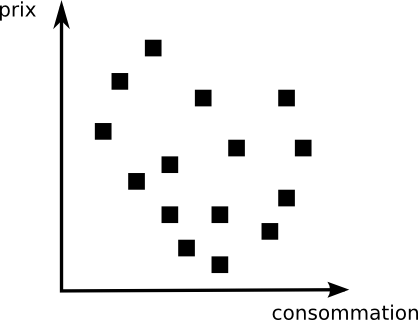
\includegraphics[width=.3\linewidth]{opti1.png}
  	\label{subfig_voiture:a}}\qquad
    \subtop[]{
	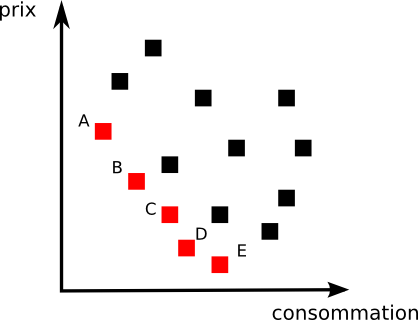
\includegraphics[width=.3\linewidth]{opti2.png}
  	\label{subfig_voiture:b}}
    \subtop[]{
  	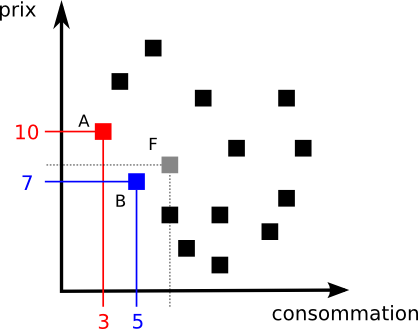
\includegraphics[width=.3\linewidth]{opti3.png}
  	\label{subfig_voiture:c}}
 \end{sidecaption}
\end{figure}

\sloppy En regardant en détail les capacités des voitures figurant dans ce front \ref{subfig_voiture:c}, on voit bien que chacune d'entre elle domine une partie des autres voitures sur au moins un des deux objectifs. Si on prend le cas de la voiture F, celle-ci n'est pas prise en compte dans les solutions optimums, car le point est dominé sur ses deux objectifs par d'autres voitures : $ prix(B) < prix(F) < prix(A) $ et $consommation(A) < consommation (B) < consommation(F)$.

Le front de Pareto renvoie un ensemble de solutions compromis optimal, l'expertise finale sur la ou les solutions à adopter est donc le résultat d'un choix expert externe introduit comme support à l'algorithme optimiseur. Dans notre exemple, l'acheteur devra pour finaliser son achat mettre en avant au moins un des deux critères afin de départager les voitures.

Si certains algorithmes ont introduit cette expertise par le biais d'une sélection interactive guidant l'optimiseur à chaque étape de sa recherche, ce n'est pas cette usage qui nous intéresse ici. L'expertise n'intervient qu'une fois les solutions convergées, dans l'observation des résultats finaux.

Dans notre cas, on considère que l'optimiseur doit sélectionner avec les moyens qu'on lui a fournis les solutions candidates sur lesquels il doit miser pour converger. Il doit donc être capable de séparer les solutions en appliquant un ou plusieurs critères de séparation. Il existe plusieurs types de stratégies (\textit{Agreggation based, Criterion based, Dominance based, Indicator based}), et chacune d'elles peut être croisée ou dérivée en de multiples variantes \autocites[28]{Zitzler1999a, Deb2001}[7]{Liefooghe2009}. Nous limiterons ici notre analyse à un seul de ces cas, en nous focalisant d'ores et déjà sur les méthodes les plus utilisées en EC, basées sur la dominance celles-ci sont directement inspirées des travaux de Pareto.

% TODO : Finir ce paragraphe historique rapide, qui permettra de faire la différence ensuite avec les algorithmes inspirés par Pareto.
% TODO : Ajouter ref de Goldberg sur les sciences humaines + GA dans le chapitre 1

\begin{figure}[!htbp]
	\begin{sidecaption}[fortoc]{Graphique en deux dimensions des fonctions objectifs $f_1$ et $f_2$ du tableau \ref{tab:pranking}}[fig:pranking_a]
		\centering  	
		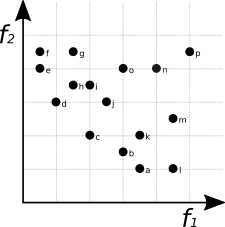
\includegraphics[width=.4\linewidth]{pareto_ranking_a.pdf}
	 \end{sidecaption}
\end{figure}

\begin{table}[!htbp]
\begin{sidecaption}[fortoc]{Tableau de résultats des fonction objectifs $f_1$ et $f_2$ pour un vecteur de solutions candidates $\{a \dotsc p\}$ dans l'espace des objectifs $\mathbb{Y}$, et résultat du \textit{Pareto Ranking}}
	[tab:pranking]
	\centering
	\begin{tabular}{>{$}l<{$}>{$}l<{$} >{$}l<{$} >{$}l<{$}}
			\toprule
			\text{solutions candidates} & f_1 & f_2 & \text{dominé par} \\
			\midrule
			a      & 3.5    & 1    &  \varnothing \\
			b      & 3      & 1,5  &  \varnothing \\
			c      & 2      & 2    &  \varnothing \\
			d      & 1      & 3    &  \varnothing \\
			e      & 0.5    & 4    &  \varnothing \\
			f      & 0.5    & 4.5  &  \{e \}  \\
			g      & 1.5    & 4.5  &  \{d,e,f,h \} \\
			h      & 1.5    & 3.5  &  \{d \} \\
			i      & 2      & 3.5  &  \{c,d,h \} \\
			j      & 2.5    & 3    &  \{c,d \} \\
			k      & 3.5    & 2    &  \{a,b,c \} \\
			l      & 4.5    & 1    &  \{a \} \\
			m      & 4.5    & 2.5  &  \{a,b,c,k,l \} \\
			n      & 4      & 4    &  \{a,b,c,d,e,h,i,j,k,o \} \\
			o      & 3      & 4    &  \{b,c,d,e,h,i,j \} \\
			p      & 5     & 4.5   &  \{a,b,c,d,e,f,g,h,i,j,k,l,m,n,o \} \\
			\bottomrule
	\end{tabular}
  \end{sidecaption}
\end{table}

Pour comprendre comment cette stratégie et définir mathématiquement la notion d'optimum de Pareto, il faut introduire la notion de \textit{dominance} sur lequel elle s'appuie. Pour cette tâche on s'appuie sur les définitions données par \textcite[65]{Weise2011} :

\foreignquote{english}{An element $x_1$ dominates (is preferred to) an element $x_2 (x_1 \dashv x_2)$ if $x_1$ is better than $x_2$ in at least one objective function and not worse with respect to all other objectives.} 

Ce qui dans le cas d'une minimisation se traduit mathématiquement par les conditions suivantes : 

\begin{align*}
	(x_1 \dashv x_2) \Leftrightarrow &\forall i \in 1 \dotsc n \Rightarrow - i f_i (x_1) \leq i f_i (x_2) \land \\
	&\exists j \in 1 \dotsc n : j f_j (x_1) < - j f_j (x_2)
\end{align*}

Cette notion de \textit{domination} ($\succ$) \Anote{notation_dominance} permet de dégager ces trois possibilités

\begin{itemize}
\item $x_1$ domine $x_2$ , qui peut également s'écrire $x_1 \succ x_2$
\item $x_1$ est dominé par $x_2$
\item $x_1$ n'est pas comparable avec $x_2$
\end{itemize}

Celle-ci possède les propriétés suivantes, qui définissent dans l'espace des objectifs $\mathbb{Y}$ un \textit{strict partial order} : 

\begin{enumerate}
\item{\textbf{non reflexive}}  $x_1$ ne peux pas se dominer lui même
\item{\textbf{non symétrique}} $ x_1 \succ x_2$ n'implique pas $x_2 \succ x_1$, alors que l'opposé est vrai, $x_1 \succ x_2$ implique $x_2$ ne domine pas $x_1$
\item{\textbf{transitive} }
\end{enumerate}

Différents degrés de dominance ont été développés, comme par exemple la notion de \textit{strong dominance} : $x_1$ domine fortement $x_2$ ($x_1 \succ \succ x_2$) si $x_1$ est strictement meilleur que $x_2$ sur tout ses objectifs. 

Pour bien comprendre comment se construit l'ensemble $X^*$ de solutions non dominées $x^* \in \mathbb{X}$ ,on peut étudier en détail comment la dominance se calcule entre les points $e$ et $f$ présentés sur la figure \ref{fig:pranking_a}.

\begin{table}[!h]
	\centering
	\begin{sidecaption}[fortoc]{Application des règles de dominance aux points $e$ et $f$. \\ \\
		   \begin{tabular}{>{$}l<{$}>{$}l<{$} >{$}l<{$}}
					\toprule
					 & f1 & f2 \\
					\midrule
					e      & 0.5    &  4   \\
					f      & 0.5    & 5,5  \\
					\bottomrule
			\end{tabular}\\ \\ 
			(a) $e \succ f$ car e est bien le meilleur sur au moins un des deux objectifs, et n'est pas pire sur aucuns des autres objectifs ($e \succeq f$ ) \\ 
			(b) f ne domine pas e car f n'est pas meilleur sur aucun des deux objectifs et il est pire sur au moins un des deux objectif}[tab:pranking]
		
		\begin{minipage}{0.5\textwidth}
			\centering
			\subbottom[e est dominé par f ?]{
				\begin{tabular}{>{$}l<{$}>{$}l<{$} >{$}l<{$}}
					\toprule
					    & f1 & f2 \\
					\midrule
					e \leq f & \text{true} & \text{true} \\
					e < f   & \text{false}  & \text{true} \\
					\bottomrule
				\end{tabular}
		 	\label{pranking_a}}
		 \end{minipage}\hspace{1em}
		 \begin{minipage}{0.5\textwidth}
		 	\centering
			\subbottom[f est dominé par e ?]{
				\begin{tabular}{>{$}l<{$}>{$}l<{$} >{$}l<{$}}
					\toprule
					  & f1 & f2 \\
					\midrule
					f \leq  e & \text{true} & \text{false} \\
					f < e  & \text{false}  & \text{false} \\
					\bottomrule
				\end{tabular}
			\label{pranking_b}}
		\end{minipage}
  \end{sidecaption}
\end{table}

Les solutions admises parmi le front de Pareto (voir figure \ref{fig:frontoptimal}) sont donc ici toutes celles qui ne sont pas dominées faiblement ($\succeq$), ce qui revient à exclure les points $f$ et $l$ du front optimum $\{a,b,c,d,e\}$ car ils sont dominés faiblement ($e \succeq f$); alors que dans le cadre d'une dominance forte ($\succ \succ$), ceux-ci auraient fait partie du front $\{a,b,c,d,e,f,l\}$. En effet si on prend toujours le cas de $e$ et $f$, la condition testant que $e$ est strictement meilleur que $f$ sur tous les objectifs n'est pas remplie. %Cet ensemble de cardinalité forcément inférieure ou égale est qualifié \enquote{d'ensemble fort non dominé} (\textit{Strongly non dominated set}).

\begin{figure}[!htb]
	\begin{sidecaption}[fortoc]{Tracé du front optimum à partir du calcul des individus non dominés, cf. l'ensemble vide $\varnothing$ dans le tableau \ref{tab:pranking}}[fig:frontoptimal]
		\centering
		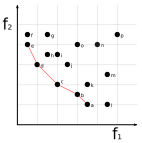
\includegraphics[width=.4\linewidth]{pareto_front.pdf}{
		}
  \end{sidecaption}
\end{figure}

Le front de Pareto n'est en général jamais entièrement couvert, cela pour diverses raisons : 

\begin{itemize}
\item L'évaluation de la fonction à optimiser est souvent coûteuse, comme dans le cas de modèle de simulation dont l'exécution peut prendre jusqu'à plusieurs dizaines de minutes, 
\item La zone d'exploration est volontairement bornée du fait des objectifs des expérimentateurs, 
\item La stochasticité oblige l'exécution de nombreuses réplications d'une même évaluation,
\item On dispose de ressources finies, or l'espace du front est souvent continu et non borné en dehors des contraintes que l'on aura nous-mêmes fixées.
\end{itemize}

Selon \textcite[70]{Weise2011} et \autocite[19]{Zitzler1999a}, on peut s'aider dans cette tâche d'établissement d'un front de Pareto correct en étant attentif aux points suivants:

\begin{enumerate}
\item{\textbf{Proximité}} Les solutions découvertes doivent être les plus proches possibles du front de Pareto optimal.
\item{\textbf{Diversité}} Si le front optimal possible est trop large, la répartition des solutions \textit{spread} doit être maximisé sur toute la surface de celui-ci, si possible suivant une distribution uniforme.
\item{\textbf{Pertinence}} Les solutions découvertes doivent correspondre aux intérêts définis par le problème, et n'ont aucun intérêt si l'opérateur humain ne peut, ou ne sait les utiliser.
\end{enumerate}

On retrouve dans ces objectifs la tension entre exploration et exploitation, le front de Pareto devant être exploité de façon homogène, tout en garantissant à terme (et si possible le plus vite possible) la convergence vers une zone d'intérêt pour l'expérimentateur (voir figure \ref{fig:convergence_diversite}). Les métaheuristiques n'ayant pas d'apriori sur la forme de problème abordée, c'est dans l'originalité, la diversité des constructions proposées qu'une solution optimale et dédiée peut être trouvée. Il est donc très difficile de faire un listing des meilleures stratégies, et des meilleures combinaisons de stratégies permettant une sélection garantie des meilleurs candidats en fonction de ces objectifs, l'établissement de cette liste ne pouvant être que contextuelle d'un problème d'optimisation donné. 

\hl{ref no free lunch theorem }? Wikipedia : Le théorème du « no free lunch » explique qu’aucune instance de métaheuristique ne peut prétendre être la meilleure sur tous les problèmes. Une métaheuristique (M) n’est performante que pour une classe de problème (P) donnée.

Heureusement, un certain nombre de combinaisons, souvent éprouvées par de multiple tests sur des fonctions aux caractéristiques et difficultés soigneusement étudiées (ZDT, etc.), se démarquent par des capacités de résolution acceptable. C'est d'ailleurs souvent sur cette première base que se construisent ensuite les améliorations nécessaires à une réponse optimale, cela en partie grâce à la flexibilité des composantes caractéristique des métaheuristiques. 

\begin{figure}[!htbp]
  \begin{sidecaption}[fortoc]{Convergence et maintien de la diversité au sein du front de Pareto}[fig:convergence_diversite]
  \centering
  \subbottom[Un front de pareto sans maintien suffisant de la diversité]{
  	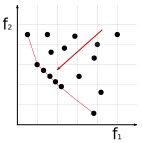
\includegraphics[width=.4\linewidth]{pareto_convergence_a.pdf}
  	\label{subfig_convergence_diversite:a}}\qquad
  \subbottom[Un front de pareto avec maintien de la diversité]{
	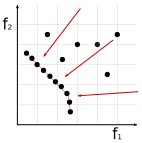
\includegraphics[width=.4\linewidth]{pareto_convergence_b.pdf}
  	\label{subfig_convergence_diversite:b}}
 \end{sidecaption}
\end{figure}

\textit{Une fois défini cet ordre partiel entre les solutions candidates évaluées, sur quelle base l'optimiseur prend sa décision pour sélectionner les individus les plus prometteurs ? et comment celui-ci garantit l'évolution des solutions candidates selectionnées au regard des trois objectifs fixés ?}

Comme le dit de façon très claire,\textcite[94]{Weise2011} \foreignquote{english}{Such comparisons, however, only state whether one candidate solution is better than another one or not, but give no information on \textbf{how much} it is better or worse and \textbf{how interesting} it is for further investigation. Often, such a scalar, relative measure is needed.}

L'optimiseur n'ayant pas les capacités pour comparer des fonctions entre elles, c'est par l'attribution d'un scalaire caractérisant chaque vecteur $z^* \in \mathbb{Y}$ résultat de l'évaluation d'une solution candidate, que celles-ci vont pouvoir être départagées. On parle de \enquote{fonction d'utilité}, ou de \enquote{fonction \textit{fitness}} pour désigner cette opération de transformation dont le résultat $z$ est utile uniquement en se plaçant dans le référentiel de l'optimiseur. Il s'agit d'un classement relatif des solutions les unes par rapport aux autres, calculés indépendamment des valeurs prises par les fonctions objectives, et intégrant un certain nombre d'autres critères, définis en réponse aux exigences des trois objectifs déjà évoqués (respect de la diversité, qualité de convergence, pertinence vis-à-vis du problème). 

Ainsi, un des tout premiers paramètres à intégrer dans le calcul de cette fonction \textit{fitness} tient évidemment dans le choix d'une stratégie pour tirer un meilleur parti des informations récoltées dans l'application de cet ordre partiel sur l'espace $\mathbb{Y}$. Là ou des algorithmes vont appuyer la sélection des solutions à partir d'un calcul de rang (je ne garde que les $n$ premiers rangs), d'autres vont le faire à partir d'un décompte des non dominés (je ne garde que les individus non dominés $< n$), à partir d'une profondeur (je ne garde que les $n$ premiers fronts), ou encore en mélangeant ces trois informations (voir le résultat du calcul de ces trois informations dans \ref{tab:pranking} \hl{a finir}) A cela il faut également ajouter la diversité de choix à disposition dans la selection d'une dominance, par le changement de l'opérateur utilisé dans le calcul (\textit{weak dominance}, \textit{strong dominance}, etc.), ou même la relaxe de celui-ci (\textit{epsilon-dominance}). Des choix de première importance, car ils interviennent directement dans la construction de l'ensemble de solution retenue.

C'est donc dans l'espace des objectifs $\mathbb{Y}$ que se révèle la première information pertinente pour l'optimiseur, nous indiquant, peu importe la forme de l'une ou de l'autre des fonctions et le positionnement des points sur celles-ci, une première sélection de solutions parmi les solutions candidates évaluées sur laquelle l'effort de l'optimiseur doit porter en priorité.

Mais lorsque l'on reprojette les résultats du front de Pareto dans l'espace figurant la dynamique supposée de chacune des deux fonctions objectifs, on observe que la prise de décision basée sur le seul ordonnancement des solutions n'est pas suffisante pour garantir une selection optimale des meilleurs candidats à l'évolution (voir figure \ref{fig:mo_landscape}). 

La forme des fonctions dans cette figure est représentée en pointillé car elle n'est qu'une description temporaire d'un paysage en partie inconnu, en attente d'être révisée par l'évaluation de nouveaux points. Le tracé d'un paysage ne se confond plus comme cela pouvait être le cas dans une optimisation mono-objectif avec la valeur prise par la fonction objectif, et doit maintenant intégrer un intermédiaire supplémentaire plus complexe qui est le calcul d'une fonction \textit{fitness}, et dont la formulation, dépendante de nombreuses stratégies, va modifier les solutions choisies dans le futur, et donc modifier la façon dont on va découvrir l'approximation de ce paysage, cela de façon indépendante aux objectifs choisis. \autocite{Weise2011}

\begin{figure}[!htbp]
	\begin{sidecaption}[fortoc]{Projection du front de Pareto optimal (point \sqbox{tangoBlack1}), et des autres solutions candidates dominées (point \sqbox{tangoGrey1}) sur l'espace de variation du paramètre $x \in \mathbb{R}$, un schéma inspiré par \textcite[67]{Weise2011}
	\parbox{\marginparwidth}{
	\begin{enumerate}[label={},labelindent=0pt,leftmargin=*]
	      \item \sqbox{tangoBlue1} $f_{1}(x)$
	      \item \sqbox{tangoRed1} $f_{2}(x)$
	\end{enumerate}}\\
	Les fonctions $f_{1}(x)$ et $f_{2}(x)$ sont représentées en pointillé car elles sont inconnues de l'optimiseur, et ne servent que de repère au lecteur pour mieux comprendre comment un paysage caractérisant l'intersection des deux fonctions peut émerger durant l'optimisation, et pourquoi cela peut être intéressant d'intégrer son analyse à l'optimiseur.}[fig:mo_landscape]
	 \centering
	 	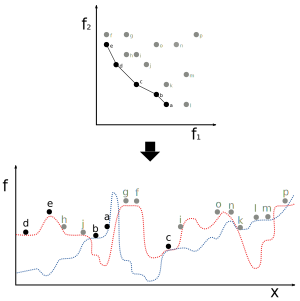
\includegraphics[width=0.8\linewidth]{multi_objective_landscape.pdf}
	\end{sidecaption}
\end{figure}

%on se rend également compte qu'un surplus d'information tiré de l'exploitation d'autres espaces pourrait être utile au choix de l'optimiseur

%\Anote{weise_multi2D}
Déjà beaucoup plus difficile à imaginer que dans l'exemple précédent de l'équation de Schaeffer, la re-projection des solutions candidates évaluées se fait sur un nouvel espace $\mathbb{G}$ (voir figure \ref{fig:relation_espaces}), qui inclu l'ensemble de tout les éléments $g \in \mathbb{G}$ qui peuvent être manipulés par les opérateurs de recherche à disposition de l'optimiseur \autocite[82]{Weise2011}. Un processus détaillé un peu plus tard dans cette section.

Dans notre cas $x \in \mathbb{R}$, on a donc un paramètre qui est manipulable et peut prendre une infinité de valeurs dans le cadre des contraintes définies pour $x$ (par exemple une valeur de 0 à 10 pour $x$) \Anote{remarque_resolution}. L'espace $\mathbb{G}$ contient la codification du problème, ce qui par exemple dans le cadre de simulation, se traduit pour chaque élément $g$ par l'attribution d'un vecteur de paramètres définissant les entrées de la simulation sur lequel l'optimiseur va pouvoir \enquote{jouer} pour optimiser les différentes fonctions objectifs.

La fonction $gpm : \mathbb{G} \mapsto \mathbb{X}$ est une translation opérée lorsque les deux espaces sont de nature différente, par exemple pour passer d'un espace Binaire à un espace de Réels $\mathbb{B} \mapsto \mathbb{R}$. Dans le cadre de simulations, les deux espaces sont souvent de nature similaire $\mathbb{G} = \mathbb{R}$. On pourra se référer à \textcite[86-88]{Weise2011} pour plus de détails.

\begin{figure}[!htbp]
	\begin{sidecaption}[fortoc]{Résumé des relations entre les différents espaces dans une optimisation}[fig:relation_espaces]
		\centering
		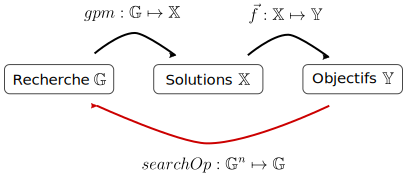
\includegraphics[width=.7\linewidth]{objectifsToSearchSpace.pdf}
  \end{sidecaption}
\end{figure}

%D'une part, l'observation de dynamiques en partie contraires sur ces deux fonctions $f_1$ et $f_2$ nous permet de constater encore une fois pourquoi un déplacement de l'optimiseur sur l'une ou l'autre des fonctions dirigé par la recherche d'un optimum n'a aucun sens. 

L'opération de sélection des solutions candidates est souvent rattachée au processus de convergence. L'objectif de l'optimiseur est d'évaluer au mieux le potentiel de chacune des solutions durant cette phase de sélection pour intégrer et conserver les meilleurs éléments à son référentiel entre deux itérations. On imagine pourtant très bien bien l'effet que peut avoir une sélection trop restrictive sur le maintien de la diversité. C'est le cas par exemple si l'optimiseur ne décide de garder que le front de Pareto, on voit bien sur la figure \ref{fig:mo_landscape} à quel point la couverture de la dynamique des deux fonctions ressortirait considérablement appauvrie à la suite d'un tel choix. On en déduit que la frontière entre stratégies de convergence, et stratégie de maintien de la diversité doit être assez perméable pour garantir le choix de solutions candidates pertinentes en dehors du seul front de Pareto. Zitler \hl{ref autre que ppt à trouver} retient par exemple parmi ces classes de stratégies celle s'appuyant sur le couple associant espace des objectifs et au choix la dominance, la densité, le temps, ou encore la chance. Ce sont des heuristiques qui vont intervenir en amont sur la qualité et la diversité des solutions candidates (par exemple les stratégies de \textit{sharing}, \textit{crowding}, etc.) qui peuvent ensuite être manipulées par les opérateurs de recherches de l'optimiseur.

Viennent ensuite les stratégies de recombinaison des solutions selectionnées, créatrices de nouvelles solutions candidates à évaluer. Un processus qui peut être là aussi rattaché tout autant au maintien de la diversité qu'à une volonté de convergence accrue. Il n'y a là encore aucune règle d'applications spécifique, et tout dépend de l'objectif fixé de façon initiale ou au cours de l'expérimentation. Ainsi, certaines stratégies intégrés aux opérateurs peuvent être mis en place pour limiter une convergence trop rapide des solutions (\textit{premature convergence}) liée à une perte de diversité, alors que d'autres vont tenter d'accélérer cette convergence par la mise en oeuvre d'opérateur de recherche plus agressif, soit pour trouver le plus rapidement possible un minimum (ou maximum) local, soit car la topologie de l'espace des objectifs est de topologie difficile. 

La sélection de candidats à la manipulation dans l'espace des objectifs $\mathbb{X}$ se réfère, une fois projetée dans cet espace $\mathbb{G}$, aux éléments $g$ accessibles à la manipulation par les opérateurs de recherche de la fonction $searchOp$. Chacun de ces opérateurs, dont le nombre et la nature est un paramètre de l'optimiseur, s'appuie sur la transformation d'une ou plusieurs solutions candidates dirigée par la création d'un nouvel élément $g$, dont on attend si possible un meilleur résultat à l'itération suivante. Un postulat très fort est posé par ce type de méthodes d'optimisation, l'introduction de petites variations sur les valeurs de l'espace de recherche est également censée apporter de petites variations dans l'espace des objectifs, que cela résulte en une amélioration ou en une dégradation de la qualité. Appelée \textit{strong causality} \Anote{note_strong}, cette propriété est évidemment dépendante de la forme prise par le paysage du problème (\textit{problem landscape}), et plus celui-ci est accidenté, rugueux, plus sa résolution est considérée comme complexe \Anote{note_weak}.

En relation avec cette observation, l'éclatement de cette population de solutions candidates évaluées sur le paysage nous permet de constater (voir la figure \ref{fig:mo_landscape}) à quel point la notion de distance entre les points parait différente entre ces deux espaces. $f$ et $c$ apparaissent ici beaucoup plus proches de trouver un optimum global que $a$ et $b$, pourtant plus proche de $c$ dans l'espace des objectifs. On voit bien ici que la sélection de solutions candidates intéressantes peut intégrer d'autres informations utiles, en supplément de celle fournit par l'analyse de $\mathbb{Y}$, au travers de l'analyse de cet espace $\mathbb{G}$; et cela toujours afin de guider au mieux l'optimiseur dans la selection des candidats à l'évolution. Un croisement du positionnement des individus $f$ et $c$ donnerait ainsi une bien meilleure valeur de $x$ à évaluer, probablement meilleure que celle d'un individu $a$ et $c$. Si la solution $f$ avait été éliminée sur le fait d'une sélection aux critères plus drastiques, c'est aussi la possibilité d'un croisement fructueux avec $c$ qui disparait.

%A ces stratégies principales s'ajoute un autre ensembles de stratégies, dont certaines sont plus spécifiques, ou constitutives des types d'algorithmes utilisés. %Le maintien d'une diversité de solutions entre les itérations fait partie de ces stratégies qui font partie d'un set plus large de stratégies permettant de contrer l'émergence des différentes difficultés (stochasticité, topologie, etc.) caractéristique d'un problème de résolution unique. 

%Généralement nommé \foreignquote{english}{Pareto Ranking} \Anote{utilisation_pareto_ranking} aussi nommé par Weise \foreignquote{english}{Prevalence Ranking}.

% Ou introduire la notion d'individu ?

\begin{figure}[!ht]
	\begin{sidecaption}[fortoc]{Résumé simplifié du déroulement d'une optimisation selon \textcite[109]{Weise2011}}[fig:resume_opti]
		\centering
		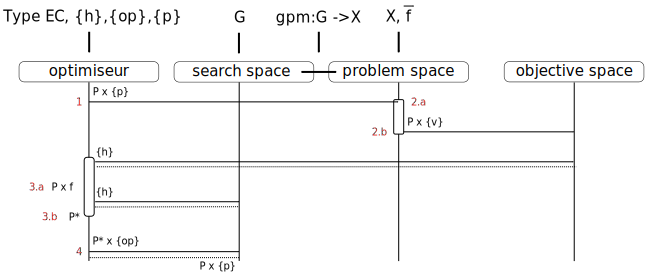
\includegraphics[width=\linewidth]{espace_resume.pdf}{
		}
  \end{sidecaption}
\end{figure}

La description des étapes de la figure résumé \ref{fig:resume_opti} sont les suivantes :

\begin{itemize}[label=\textbullet]
	\litem{1} Une première population $P \in {1 \dotsc n}$ de vecteurs paramètres ${p}$ est générée par l'optimiseur ou introduite par l'expérimentateur, puis soumis à évaluation.
	\litem{2.a} La fonction à optimiser est évaluée autant de fois qu'il y a de vecteurs ${p}$ 
	\litem{2.b} Les fonctions objectifs $\vec{f}$ sont calculés, ce qui permet de créer autant de vecteur ${v}$ correspond au résultats des fonctions qu'il y a de $P$ évalué. Ces vecteurs $P(v)$ peuvent être positionné dans un espace des objectif $\mathbb{Y}$ 
	\litem{3.a} Le calcul de fitness $f$ est effectué pour chaque élément de $P$ en utilisant les informations rapportés par un ensemble d'heuristiques sur $\mathbb{Y}$ et, ou $\mathbb{G}$
	\litem{3.b} A partir du calcul de cette fitness $f$ pour chacun des éléments de $P$, on selectionne les $P^*$ meilleurs éléments.
	\litem{4} A partir d'un ensemble d'opérateur ${op}$ on va générer de nouveaux vecteurs de paramètres $P(p)$, qui va constituer le nouveau jeu de solution candidates à évaluer à l'étape (1), et dont on espère qu'elles seront si possible meilleures que les précédentes.
\end{itemize}

\hl{Manque la notion d'invididu = fitness + genotype + phenotype}

% Injection de connaissance se fait un peu partout pour la construction d'une fitness.

% Penser à dire qu'il y a plusieurs stratégies de comparaison autre que Pareto ? 

%Première fois utilisé en 1989

%Si on transfère ce langage neutre au vocabulaire que l'on peut trouver courrament dans l'EC, alors l'espace des solution devient le \textit{phenome}, et le point de cet espace qui correspond à la solution candidate devient un \textit{phenotype}.

%\begin{figure}
%\begin{sidecaption}[fortoc]{ POM cycle for developping theory for an agent behavior \autocite[245]{Railsback2012}}[fig:S_syntheseGrim]
%  \centering
% 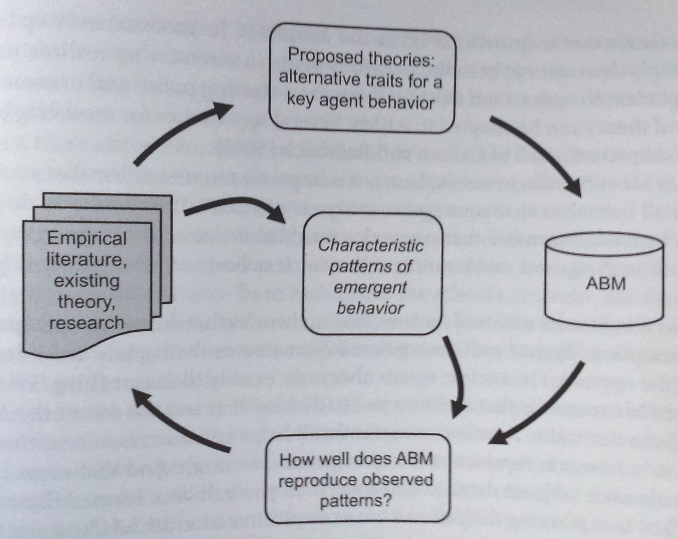
\includegraphics[width=.9\linewidth]{cyclePOMcomportement.png}
%  \end{sidecaption}
%\end{figure}


%Dans notre étude, l'objet à optimiser ne se réfère pas à une expression mathématique, mais à un modèle de simulation, sur lequel on va déterminer un ensemble de critères qui vont faire figure d'équivalent de ces fonction objectives. Dans ce cas d'utilisation, l'optimisation est plus souvent employé comme une forme de calibration inversé \autocite{Grimm2011}, dans laquelle on cherche à déterminer si il existe un ou plusieurs jeu de valeur de paramètres du modèles de simulation respectant la plage de valeur viable empiriquement qui permettent de maximiser l'obtention d'un ou de plusieurs critères experts. Il est plus parlant dans notre cas de désigner l'espace de recherche comme l'espace des paramètres.  

La branche des métaheuristiques EC que nous allons étudier plus spécifiquement s'appuie sur l'observation de phénomènes naturels, comme l'évolution, ou l'organisation, pour la construction et la mise en oeuvre d'algorithmes mimant certaines propriétés intéressantes de ces processus, cela sans être rattaché à une contrainte de réalisme biologique.

\subsection{Les métaheuristiques bio-inspirées, la branche des Algorithmes Evolutionnaires}

\subsubsection{Un rapide historique de la discipline}

On a déjà rapidement décrit dans la section à propos de l'Artificial Life \ref{p:heritage_complexe} les deux voies qu'il était possible d'emprunter dans l'intéret porté sur la définition du processus naturel d'évolution. 

Il existe en effet au moins deux façons aujourd'hui d'introduire des développements informatiques se rapportant à ce processus évolutif. D'un côté, les tentatives de reproduction plus ou moins fidèles des différents mécanismes à l'oeuvre dans le processus d'évolution mettent en avant un objectif de compréhension, alors que la focalisation sur ces mêmes mécanismes pour leur seule capacité d'apprentissage tend à s'éloigner de la réalité biologique pour s'orienter plus vers le développement d'algorithmes désignés comme métaheuristiques. Autrement dit, là ou des chercheurs vont tenter de reproduire au mieux le processus d'évolution dans ce qu'il a de créatif, de non optimisé, de coévolutif car construit par \Anote{note_pattee_semantic_closure} et avec l'environnement, d'autres vont reprendre ce même processus en vue d'une évolution si possible bornée et dirigée par la résolution efficace d'un ou de plusieurs objectifs définis de façon fixe et extrinsèque \autocites{Taylor2001, Taylor2012}.

Lorsqu'on s'intéresse de plus près à la littérature scientifique de ces algorithmes regroupés depuis Fogel sous le terme d'\foreignquote{english}{Evolutionary Computation} (EC), on constate pour toute une partie des publications une de-contextualisation complète de leur utilisation. La question d'une similitude initiale avec le vivant n'étant le plus souvent évoquée que pour illustrer des racines historiques éloignées. Ce qui peut apparaitre comme une forme de surspécialisation est en quelque sorte le prix à payer d'une évolution de la discipline avant tout dirigée par une communauté de chercheurs informatiques motivés par la recherche d'algorithmes performants et d'applications génériques.

Si aujourd'hui on peut observer un tel cloisonnement, un regard sur l'histoire de la discipline tend à montrer tout l'inverse, car nombreux sont les pionniers ayant développé des intérêts simultanés pour ces deux approches : les expériences très longtemps restées inconnue du mathématicien Barricelli dès 1954 \Anote{barricelli_multi_utilisation}, l'approche du généticien \textcite{Fraser1957} qui décrit et simule l'évolution de population génétique dès 1957 \Anote{fraser_comment}, les travaux de Pattee et Conrad avec EVOLVE à la fin des années 1960 \autocite{Conrad1970}, les algorithmes génétiques \Anote{holland_multi_utilisation} de Holland, un élève de Burks, un scientifique dont on a déjà vu dans le paragraphe \ref{p:va_automate_cellulaire} qu'il était proche de Von Neumman.

Il existe toutefois une littérature scientifique parallèle qui continue de motiver la rencontre autour de disciplines scientifiques ayant un intérêt pour la recherche en \textit{Artificial Life}. C'est le cas par exemple de la biologie, ou de l'écologie \autocite{Hamblin2013} qui organisent autour de publications transverses la réflexion sur la reintroduction des outils tel qu'ils sont développés en informatique, entrainant de fait aussi la création et l'évolution de ces derniers \autocite{Hogeweg2011}. C'est également le cas en biologie, ou on imagine l'importance que peuvent avoir les travaux de \textcites{Taylor2001}[221]{Taylor1999} pour la mise en oeuvre de modèles de simulation dirigés vers l'émergence \enquote{créative} de nouveaux phénotypes dans un environnement ouvert \autocite[33]{Taylor1999}. Une critique récurrente adressée aux modèles d'auto-organisation actuels \autocite{Pumain2003}, encore incapables de simuler l'émergence de nouvelles structures, de nouvelles entités de façon crédible. Une autre forme de relation entre les deux approches est également envisageable dans certaines disciplines, comme en écologie, où celles-ci peuvent parfaitement se côtoyer : \foreignquote{english}{The first of these requires the application of the evolutionary process in much the same way as it has been traditionally applied within A-Life: as a means to dynamically adjust agent parameter values to support their viability and reproduction within the virtual environment. [...] The second approach we suggest employs artificial evolution to match simulation patterns against data gathered from the level of specific species up to data concerning specific ecosystems. Once the parameters of the system have been optimised so as to reproduce the patterns observed in field data, the evolution algorithm is turned off. The model may then be employed to answer questions relating to the specific ecosystem and species that it represents. Unfortunately it may not then be used to study the evolution of these specific species in specific environments. This is a shortcoming of the artificial evolution algorithm (it does not model real evolution in detail) that would be worth overcoming.} \autocite{Dorin2008}

Le lecteur souhaitant obtenir une vue plus globale des différents concepts et ramifications disciplinaires réunit sous le terme parapluie d'\textit{Artificial Life} peuvent se référer à l'article d'\textcite{Aguilar2014} qui concentre un grand nombre d'entrées bibliographiques essentielles pour aborder les entrées de cette thématique dans chacune des disciplines. On trouvera également une description plus précise sur l'histoire commune de ces deux voies de recherches, telles quelle est perçues par les acteurs historiques de l'EC, dans les ouvrages de \autocites{DeJong2006a, Fogel1998, Fogel2006a, Fogel2006b, Back1996, Back1997}.

Dans cette section, c'est bien la deuxième branche de recherche qui est suivie, celle visant l'\enquote{optimisation}. Les développements tels qu'ils sont abordés ne se mesurent donc plus en fonction d'un critère de réalisme biologique, mais en fonction de critères informatiques et mathématiques se rapportant plus à la capacité de résolution des algorithmes, et aux supports de mise en oeuvre et de mesure de ces derniers : rapidité, diversité, robustesse, qualité, etc.

\textcite{DeJong2006a} retient trois foyers importants pour le développement de cette deuxième branche dans les années 1960, la \textit{Technical University} de Berlin avec Rechenberg, Biernet et Schwefel \autocite{Beyer2002}, UCLA à la même période avec Lawrence J. Fogel, et l'université du Michigan avec John Holland.

De ces trois branches vont émerger au cours des années 1970 ce que \textcite{DeJong2006a} qualifie comme des \foreignquote{english}{Evolutionary Algorithms (EA)} canoniques. Autrement dit, ce sont des algorithmes matures, qui ont prouvé leur capacité à produire des solutions dans un contexte précis : \foreignquote{english}{Evolutionary Programming (EP)}, \foreignquote{english}{Evolution Strategy (ES)}, \foreignquote{english}{Genetic Algorithm (GA)}

Ils vont représenter chacun le foyer d'un développement qui va s'accélérer dans les années 1980, avec l'amorce d'une popularisation de ces techniques permises entre autres par l'avènement de capacités de calcul plus conséquentes et la reconnaissance de l'efficacité de ces algorithmes pour la résolution de problématiques industrielles plus concrètes. L'ouvrage de synthèse écrit par \textcite{Goldberg1989} contribue de façon très importante à cette diffusion, et constitue également un apport théorique important dans la naissance de la branche multi-objectif de cette discipline.

Les années 1990 vont quant à elles consacrer la rencontre et l'unification de ces différentes approches restée jusqu'alors assez indépendantes si on en croit \textcite{DeJong2006a}. De cette confrontation nait la reconnaissance d'un seul terme fédérateur, l'\textit{Evolutionary Computation (EC)} motivant alors la création de nouvelles conférences et de nouveaux journaux structurant cette nouvelle discipline. C'est aussi à partir de cette période que l'on observe la mise en place d'une hybridation accélérée entre les différentes approches qui s'accompagne d'une forme de remise à plat théorique et l'émergence d'un cadre de réflexion unifié. \autocites[23-31]{DeJong2006a}{Back1997}

Si on se concentre plus précisément sur la branche multi-objectif de la discipline, la première introduction théorique d'une stratégie s'appuyant sur le calcul de l'optimum de Pareto pour définir un classement original des solutions évalués est présenté à la page 197 de \textcite[197]{Goldberg1989}. Cette technique nommé \textit{Non Dominated Sorting} (NDS) \autocite[40-43]{Deb2001}, probablement la plus efficace et plus célèbre, sera reprise et implémenté presque dix ans plus tard en 1994, dans l'algorithme célèbre NSGA (Non dominated Sorting Algorithm) de Deb et Srinivas.

Les travaux de \textcite{Goldberg1989} ont influencé tout une génération de chercheurs à partir de cette simple ébauche théorique de tri basé sur la dominance de Pareto, et nombreux sont ceux qui se sont par la suite appuyés \autocite[175, 235]{Deb2001} sur les informations du calcul de dominance pour développer diverses stratégies d'attribution de \textit{fitness}, comme MOGA (Fonseca et Flemings 1993), NPGA (Horn et Nafpliotis 1994), NSGA (Deb et Srinivas 1994), et bien d'autres \autocite[14]{Zitzler1999a}. Ce que l'on peut considérer comme la génération suivante d'algorithmes, que \textcite{Coello2006} \Anote{coello_note} fait démarrer avec l'apparition de l'élitisme \Anote{note_elitisme}, est plus axée encore sur l'efficacité de ces derniers avec notamment l'ouverture d'une branche de recherche développant des métriques de performance, et de nouveaux standards de mesures \autocites{Coello2006, Zitzler2003}, dont on s'aperçoit qu'elles sont devenues nécessaires pour comparer correctement les algorithmes entre eux \autocite[14-15]{Zitzler1999a}. Parmi ces nouveaux algorithmes, devenus depuis canonique, on trouve PAES (Knwoles and Corne 2000), SPEA (\autocite{Zitzler1999}), ou encore NSGA 2 (Deb 2000) etc. On trouve à ce sujet un état de l'art et des exemples de calculs à la main pour ces différents algorithmes dans un des premiers et très bon ouvrage de synthèse de \textcite{Deb2001}, aux chapitres 5 et 6. Il est toutefois à noter, comme le fait déjà Golberg en 1989, que cette problématique de recherche d'une solution à un problème multi-critères, puis multi-objectifs est d'origine bien plus ancienne, et a pu servir de support à la mise en oeuvre de techniques plus ou moins similaire à celle de Pareto. Ainsi, les premières traces en EA d'un intérêt théorique et parfois pratique de ces problèmes semblent remonter à Box et Draper (1957), Fogel (1966), Rosenberg (1967) \autocite[174-175]{Deb2001}. Mais la première implémentation informatique est en général attribuée à David Schaffer, avec son travail de thèse (1984) et l'implémentation de l'algorithme d'optimisation VEGA (\textit{Vector Evaluated Genetic Algorithm}). Un autre état de l'art sur l'optimisation multi-objectifs s'appuyant sur Pareto en dehors des techniques purement évolutionnaire est également possible. C'est grâce à l'existence de ce cadre formel mathématique permettant la description d'un problème d'optimisation, tel que nous l'avons un peu abordé dans la section précédente en s'appuyant sur les écrits de \autocite{Weise2011}, que \textcite[50-79]{Deb2001} indique par exemple comment certaines de ces stratégies hors EC ont été pour certaine également transférées avec plus ou moins de succès aux EA \textcite[171-237]{Deb2001}.

Enfin on notera qu'il existe également une autre classe proche d'algorithmes d'optimisation basée sur une observation des mécanismes naturels, celle-ci n'étant plus basée sur la métaphore évolutive par reproduction (même si l'hybridation est envisageable), mais sur les capacités d'organisation et d'auto-organisation observées chez certains animaux comme les fourmis, les abeilles. Ces comportements ont d'abord inspiré les développements de plateformes informatiques adaptées à l'émergence de ce type de comportements, avant d'être repris et utilisé de façon beaucoup plus abstraites par la suite pour résoudre des problèmes d'optimisation. Aujourd'hui regroupées sous le terme de \foreignquote{english}{Swarm Intelligence}, ce sont par exemple les algorithmes PSO (Particle Swarm Optimization), ACO (Ant Colony Algorithms), ABC (Artificial Bee Colony), etc.

\subsubsection{Les principes sous-jacent aux EA}

Afin de pouvoir mettre en oeuvre la possibilité d'une telle souplesse dans l'adaptation de l'algorithme à une problématique d'optimisation donnée, \textcite[49]{DeJong2006a} a considéré la construction d'un modèle conceptuel plus abstrait capable d'englober dans sa description les mécanismes d'au moins ces trois version canoniques GA, ES et EP. Les concepts clef qui se dégagent d'une telle prise de distance peuvent ainsi être repris non seulement pour décrire les version canoniques mais également pour développer de nouvelles variantes ou extensions d'algorithmes. 

Les éléments communs retenues sont les suivants :

\begin{itemize}
\item Une population de taille constante $m$ évolue au cours du temps
\item La population courante est utilisée comme une source de parents pour produire une progéniture (\textit{offsprings}) de taille $n$
\item La population étendue ainsi constitué est réduites de $m + n$ à $m$ individus.
\end{itemize}

% En général puis recentrage sur les détails ?
\paragraph{Les avantages et les inconvénients d'une terminologie spécifique}

En 2014 une publication sur le blog du spécialiste de la discipline Thomas Weise's \Anote{billet_weise} revient longuemment sur les problématiques de ce vocabulaire inspiré par la biologie et ancré dans les différentes branches composantes l'EC. Il retient quatre problématiques dans l'usage de cette terminologie, parmi lesquels l'incompatibilité des terminologies entre les différentes branches, la dissonance entre la terminologie et la réalité d'application des algorithmes, le fait que l'optimisation au sens naturel n'est pas forcément une bonne optimisation, le fait également que cette terminologie sonne comme anti-profesionelle \Anote{note_pengouin}. Le plus grand problème étant dans ce cadre l'invention de néologisme ne faisant référence ni au domaine biologique, ni au domaine informatique. Ce n'est pas la seule voix à se faire entendre sur ce sujet, comme l'article de \textcite{Sorensen2012b} qui pointent clairement les dérives néfastes associées à l'usage systématique et surtout non réellement argumentée de nouvelle analogies ou métaphores, que celle-ci soit biologique ou pas ...

Si la perspective d'un changement d'annotation et de vocabulaire est probablement conçu comme une étape majeure dans la progression et l'unification d'une discipline depuis quelques années déjà sur la voie de la maturité, Weise tout en pronant au maximum la bonne parole continue comme beaucoup d'autres à utiliser cette terminologie \autocite{Weise2011}, très ancrée dans un folklore qui tient à l'historique de la discipline. La librairie logicielle MGO décrite par la suite s'appuie elle aussi sur cette terminologie, aussi nous n'utiliserons donc les terminologies alternatives proposés par Weise que sous forme de complément, afin de ne pas introduire trop de distance entre les termes décrivant les algorithmes dans ce manuscrit et la réalité du programme tel qu'il est conçu pour le moment.

\begin{table}[!htbp]
\begin{sidecaption}[fortoc]{Tableau de correspondance entre les notations à consonnance biologiques et les notations plus génériques liés à l'optimisation, lorsque celles-ci existent. Une traduction appuyée sur la section précédente, et les travaux de \textcite{Weise2011}}
	[tab:ptraduction]
	\centering
	\begin{tabular}{ll}
		\toprule
		générique & biologique (FR)\\
		\midrule
		Espace du problème ($\mathbb{X}$) & Phénome \\
		Espace de recherche ($\mathbb{G}$)   &  Génome \\
		Point dans un espace de recherche ($g \in \mathbb{G}$) & Génotype \\
		Solution candidate, Point dans un espace de solutions ($x \in \mathbb{X}$) & phénotype \\
		Opérateurs de recherches ($searchOp$) & Reproduction \\
		Opérateur de recherche Unaire & Mutation \\
		Opérateur de recherche Binaire & Crossover \\
		Itération & Génération \\
		?  & Progéniture \\
		?  & Mating pool \\
		\bottomrule
	\end{tabular}
  \end{sidecaption}
\end{table}

\paragraph{Les avantages et les inconvénients}

Origine : Deb2001, Fogel2000, Back1997, \autocite[104,105]{DeJong2006a}

\begin{enumerate}[label=(\alph*),labelindent=\parindent,leftmargin=*]
	
	\item Evaluation d'une population entière par génération, ce qui n'est pas le cas de nombre de techniques fournissant une seule solution par execution d'algorithme.
	\item Facile à paralléliser, une propriété étudié très tot, voire \autocite[444]{Alba2002} 
	\item Ne demande a priori aucune connaissance de la forme du paysage, même si en réalité c'est un plus pour bien choisir et paramétrer les métaheuristiques
	\item Applicable à des problèmes continus, discrets, ou les deux.
	\item Ne demande pas forcément de repartir de zéro entre chaque analyse en comparaison à d'autres algorithmes
	\item Le nombre de degré de liberté pour modifier une métaheuristique est très important, ce qui augmente les chances de trouver une combinaison adapté à un problème complexe donné
	\item Les principes de mise en oeuvre sont relativement facile à comprendre
    \item Efficace, même sous une forme canonique
    \item Capacité à explorer de très large espace de recherche
\end{enumerate}

Désavantages, limitations : 
\begin{enumerate}[label=(\alph*),labelindent=\parindent,leftmargin=*]
	\item le fonctionnement reste opaque, et le résultat n'est souvent pas tractable mathématiquement
	\item Stochasticité demande réplication
	\item Non garantie d'un optimum global
	\item Le nombre de degré de liberté demande une certaine forme expertise pour en tirer le meilleur partie, la construction d'un EA optimal pour un problème donné étant progressif, incrémental
    \item Trop facile à comprendre, il en résulte une certain illusion quant au capacité \enquote{magique} de ce type d'algorithme.
    \item Necessite une source conséquente de puissance pour réaliser de grand nombres de calculs en parallèle 
    \item Meme si les résultats sont meilleurs avec ce type d'approche, celle(ci a ses limites, et les performances se dégrade avec l'augmentation de l'espace de recherche (dimensionalité) et ou le nombre d'objectifs (limite de l'approche Pareto) Zitzler1999a page 24 cite Fonseca Flemming 1995
\end{enumerate}

Optimisation de paramètres est un domaine d'application reconnu des EA du fait aussi de la facilité de mapping entre vecteur de paramètres et génome \autocite[83]{DeJong2006a}

Dans la lignée des objectifs définis dans le chapitre 3, cette branche spécifique des EA est celle qui est à la fois la faciles d'accès en terme de compréhension pour les débutants tout en restant également suffisament de flexibilité et d'efficacité pour convenir à notre utilisation. 

De plus certains désavantages sont de conséquences plus limités dans le cadre de nos objectifs. En effet, pour le profil d'utilisateur modélisateur que nous visons la garantie d'un optimum global n'est pas la priorité immédiate en comparaison de l'importance d'accéder rapidement à des premiers résultats via un premier EA générique exécutable, qu'il pourra de toute façon ensuite améliorer du fait de la nature métaheuristique de ces algorithmes. De façon similaire, le fait que le résultat ne soit pas tractable mathématiquement n'est pas vraiment problématique dans le cadre des systèmes complexes, ou ce type d'observation est justement une propriété récurrente des systèmes que l'on cherche à simuler pour mieux les comprendre. 

Enfin, il est important de noter que cette classe d'algorithmes accueille les approches les plus efficaces pour la résolution de problèmes multi-objectifs, une propriété courante des problèmes abordés dans notre discipline, car les modèles de simulation construisent souvent leur crédibilité aux croisements de multiples critères. (\hl{POM, cf problème inverse calibration déjà expliqué plus haut})


\hl{/..../}


\hl{Introduction à un algorithme simplifié, soit sous forme d'algorithme, soit sous forme de schéma}

\begin{algorithm}[H]
 \KwData{this text}
 \KwResult{how to write algorithm with \LaTeX2e }
 initialization\;
 \While{not at end of this document}{
  read current\;
  \eIf{understand}{
   go to next section\;
   current section becomes this one\;
   }{
   go back to the beginning of current section\;
  }
 }
 \caption{How to write algorithms}
\end{algorithm}

Chacun de ces items ouvre quasiment la voie à des sous domaines d'expertises spécifiques. Voici un apercu cumulatif des élements susceptibles de varier d'un algorithme à un autre, et d'une application à une autre, dont certain sont hérités de la nature métaheuristique des EC, puis de la nature spécifique des EA, et enfin de la nature multi-objectifs (*) : \autocite[69,72,115]{DeJong2006a}[264-269]{Weise2011}[91]{Liefooghe2010} : 

\begin{itemize}
\item la stratégie de représentation interne d'une solution 
\item la stratégie d'initialisation et de maintien d'une ou de plusieurs populations
\item les stratégies de sélection des parents pour la reproduction
\item les stratégies de réintroduction des enfants dans la ou les population(s)
\item le groupe d'opérateurs choisi et la stratégie d'utilisation de ces opérateurs dans le processus de reproduction
\item le choix d'une fonction de translation \textit{gpm} entre $\mathbb{G}$ et $\mathbb{X}$
\item (*) les stratégies de préservation de la diversité
\item (*) les stratégies élitiste de selection et de maintien des survivants
\item (*) la méthode d'attribution d'une \textit{fitness} $v$
\item le critère d'arrêt
\end{itemize}

Si cette liste de classe de choix permet de cerner de façon plus globale les questions à se poser lorsqu'on construit ce type d'algorithmes, cette représentation est encore trop vague, trop linéaire, et ne rend pas compte de la plasticité et des contraintes voulu ou imposé par la construction dynamique d'un algorithme véritablement adapté au problème. Les dépendances entre éléments de la liste n'apparaissent pas dans cette représentation, or pour chacun des choix réalisés par l'expérimentateur a lieu un recalcul des degrés de liberté, ce qui entraine l'apparition ou la disparition de nouveaux choix, en fonction des dépendances existantes entre chaque éléments. \Anote{reflexion_DeJong}

Par exemple, le choix d'une représentation interne d'une solution sous forme de vecteur de binaire, réel ou encore mixte, de taille dynamique ou fixe, doublé ou non de paramètres spécifiques de convergence, joue de façon assez logique sur les choix disponibles dans chacunes de ces classes. Ainsi le groupe d'opérateurs choisi pour manipuler ces vecteurs lors de la reproduction ne seront pas les même selon qu'on manipule des éléments Binaires ou Réels.

De plus, il faut imaginer que chaque stratégie est accompagnée de son lots de paramètres associés, et ce n'est qu'à terme d'une construction, lorsque le choix d'une combinaisons d'éléments est actée que la liste de paramètres définitives apparait de façon claire à l'expérimentateur.

Enfin, dans notre cas, où il est question d'utiliser ces algorithmes évolutionnaires en s'appuyant sur toute la puissance informatique disponible, de nombreux nouveaux choix \autocite[221-224]{DeJong2006a} émergent à la lumière des modèles plus poussé de parallélisation des EA. Par exemple la mise en place d'une stratégie de parallélisation en ilôts, dont on verra un peu plus loin qu'elle est optimale pour une utilisation sur une grille de calcul, pose les nouvelles questions suivantes :

\begin{itemize}
	\item quels sont les stratégies de migration des individus entre les différentes populations ?
	\item combien d'ilots sont nécessaires ?
	\item les population initiale des ilots est elle identique ou différente ?
	\item quelle topologie d'ilot est la plus adaptée ?
	\item etc.
\end{itemize}

C'est un aperçu des problèmes que nous tenterons de résoudre avec la construction d'une librairie logicielle à l'architecture originale, couplé avec openMOLE pour gérer la partie parallélisation, et qui sera exposée dans les sections suivantes.

Une partie de la modularité inhérente aux métaheuristiques a déjà pu par chance être saisie dans le développement de nombreuses librairies logicielles, il est alors légitime de se poser la question suivante, pourquoi développer et surtout maintenir une nouvelle librairie ? 

Les raisons de ce choix sont guidées par une observation critique des librairies existantes, et la volonté de satisfaire au mieux les critères évoqués dans le chapitre 3 \hl{ref section}.

Il est question de mettre en place une librairie de construction d'algorithmes évolutionnaires, exposant une syntaxe lisible exposant le schéma interne d'algorithmes connus et des plus efficaces pour résoudre des problèmes d'optimisation. Destiné à un public novice, 


\paragraph{Expression au niveau de l'expérimentation : }

\begin{enumerate}

\item{Besoin de plus de flexibilité ?} 

\end{enumerate}



Qu'est ce qui fait la facilité de prise en main ? Respecter les pratiques existantes, tout en étant offrant des solutions alternatives lorsque le modélisateur en a besoin. 

\paragraph{Au niveau utilisateur, cas d'utilisation orienté vers les métaheuristiques}

\begin{enumerate}

	\item{\textbf{Besoin de plus de flexibilité ?}} L'algorithme évolutionnaires proposé en l'état ne donne pas de bons résultats, le programme doit permettre d'accéder \textbf{facilement} à toute la combinatoire offerte par la variation des différents composants intégrant cette branche des métaheuristiques. 

	\item{\textbf{Besoin de plus de puissance ?}} Fonctionnel sur une machine standard, les algorithmes évolutionnaires doivent pouvoir tirer parti de ressource informatique plus importante de façon locale (multi-coeur) ou distribué (cluster, grille de calcul), et cela en utilisant les méthodes adaptés. Ce passage d'une execution locale à une execution distribué doit être possible \textbf{facilement}.

	\item{\textbf{Besoin de plus d'extensibilité ?}} Je ne trouve pas le composant nécessaire à la construction d'une métaheuristique adapté à mon problème, quels sont les outils mis à ma disposition pour que je puisse ajouter le ou les composants facilement, à moindre cout, sans que l'ensemble du programme ne soit affecté par mes modifications. 

\end{enumerate}

\paragraph{Au niveau utilisateur, cas d'utilisation orienté vers le couplage (simulation - metaheuristique) }

\begin{enumerate}

	\item{} Mon modèle évolue pour changer de plateforme (Netlogo -> Gamma), mais l'optimisation et les paramètres de l'optimisation reste si possible en place et fonctionnel.
	\item{} Existe-t-il une bibliothèque d'expérimentations comportant un ou plusieurs exemple ou patron(s) pour une utilisation du modèle de simulation avec des métaheuristiques ?
	\item{} Comment sont définit les fonctions objectifs ?
	\item{} Comment sont définit les mapping entre paramètres du modèles et représentation interne d'une solution ?
	\item{} Est ce que ces fonctionalités sont accessible par une manipulation interactive ou par le biais de scripts ?

\end{enumerate}

% MODYSS !

\paragraph{Au niveau technique}

- Modulation de l'accès à la puissance informatique indépendante du modèle : Intégré à OpenMOLE, le couplage doit apparaitre comme transparent, tout en restant hautement flexible ce qui suppose l'existence de primitive de plus haut niveau qui assure la partie parallélisation nécessaire à l'usage confortable de tels algorithmes.


- Découpler les plateformes de simulation 
- Supporter différents niveau de parallélisme au niveau des métaheuristiques

- La facilité d'ajout de nouveaux composants
- Une bibliothèque d'algorithmes canonique à disposition
- La documentation 

Dans l'association entre modèle de simulation et métaheuristique : Modalités de jointure entre le modèle de simulation \enquote{tel qu'il est développé} et la librairie d'algorithme évolutionnaire.

- Séparation entre modèle de simulation 
- 

Deux phases ? 
- Usage indépendant
- Usage associé à openMOLE



fait apparaitre l'optimisation comme une étape supplémentaire dans l'expérimentation, 

%BehaviorSearch follows in the tradition of NetLogo [Wilensky, 1999, 2001; Tisue & Wilensky, 2004], and Logo [Papert, 1980] before it, in embracing the twin design goals of “low threshold” and “high ceiling”. By this we mean that the BehaviorSearch tool should be both easy for beginners to learn and use (“low threshold”), while also providing advanced features that will allow expert modelers to engage in cutting-edge research and analysis (“high ceiling”). To be clear, the “low threshold” goal for NetLogo, which aims to support use by elementary school students, is lower than that of BehaviorSearch, which primarily targets NetLogo’s research audience. However, increasingly NetLogo is being used by undergraduates or even high school or middle school students who are developing agent-based models for research projects, and we would like BehaviorSearch to be accessible to these audiences, as well as researchers from various disciplines who are non-expert programmers but have adopted ABM methodologies for their research. Just as NetLogo strives to make the creation of agent-based models accessible to children and novices, BehaviorSearch aims to facilitate model analysis by making search and optimization techniques accessible to all modelers.

State of the Art
Flexibilité

Facilité de parallélisation 
Facilité de construction

\subsection{Un point rapide sur les solutions EC existantes}

Les librairies logicielles permettant la mise en oeuvre d'algorithmes évolutionnaires existent dans de très nombreux langages informatiques. Les \textit{Survey} ou \textit{state of the art} sont régulièrement mis à jour dans cette discipline, et il est inutile de se substituer ici à ce type de travaux en évoquant les avantages et les inconvénients comparés de toutes ces librairies. Le lecteur pourra se référer à l'étude très complètes de \textcite{Parejo2012} comparant selon 271 critères 11 des plus importantes plateformes sur les 33 qu'ils ont identifiés. De notre coté, on se contentera d'illustrer ce que l'on considère comme les principaux défaut du point de vue de notre grille de lecture en selectionnant un ou plusieurs librairies parmis les plus usités.

Un premier filtre permet d'éliminer toute celle qui ne s'adresse qu'à une seule branche des EA, ou qui n'implémente aucun des algorithmes multi-objectifs. 

Un deuxième filtre permet d'éliminer également toute les librairies qui sont intégrés à un logiciel, impossible à utiliser en dehors de celui-ci. Le cas particulier des logiciels de modélisations (simulateurs) intégrant des algorithmes EC sera toute de même abordé afin de situer les limites de ces approches.

Un troisième filtre, 

Afin de satisfaire les objectifs que nous avons fixés, la librairie doit pouvoir fonctionner avec OpenMOLE, car une des tâches de ce dernier va être d'orchestrer de façon transparente la parallélisation de ces algorithmes evolutionnaires, ce qui suppose une interaction assez fine entre les deux outils, et un langage informatique compatible avec Java ou Scala, les langages sur lequel est construits OpenMOLE.


\subsubsection{Les librairies standards}

Apache Commons

\href{http://www.moeaframework.org/}{@MOEAFramework}

\href{http://dev.heuristiclab.com/}{@HeuristicLab 2002 .Net CSharp Microsoft dependent}

\href{http://jmetal.sourceforge.net/}{JMetal (2010)}

\href{http://image.diku.dk/shark/sphinx_pages/build/html/index.html}{Shark machine learning library (c++)}

\href{http://www.tik.ee.ethz.ch/sop/pisa/?page=documentation.php}{PISA (C / C++) 2003}

Paradiseo-MOEO et Paradiseo-PEO (C ++)
Logiciels de l'INRA

\href{http://cs.gmu.edu/~eclab/projects/ecj/}{ECJ (1998) (orienté GP)}

\href{http://opt4j.sourceforge.net/}{Opt4J (Java) 2011}

\href{http://esa.github.io/pygmo/}{Pygmo (Python) PaGMO (C++) (ESA)}

\href{http://jgap.sourceforge.net/}{JGAP}

\subsubsection{Les approches intégrées}

\paragraph{Le {BehaviorSearch} de Stonedahl}

La librairie \textit{BehaviorSearch} developpé par Railsback pour Netlogo intègre une librairie d'algorithme génétique.

Les solutions existantes de couplage, comme le \textit{behavior search} déjà évoqués dans \hl{la section XX}, ne sont pas entièrement satisfaisantes, cela sur plusieurs points déjà évoqués et résumé ci dessous, auquels on rajoute de nouveaux inconvénients propre à la manipulation avancé des métaheuristique : 

a) Le cycle de vie d'un modèle ne se limite pas forcément à l'établissement d'un seul modèle Netlogo, mais plusieurs, et de complexité différentes. Si Netlogo est un outil indispensable de par la force et la rapidité de concrétisation d'une idée scientifique qu'il permet, les scientifiques non développeur peuvent rapidement être piégé par des problématiques tenant plus de la science informatique que de leur domaine initial. 

b) Le niveau de prise en charge de l'expérimentation est insuffisant pour assurer une recherche reproductible au delà du seul modèle. Par là il faut comprendre que le protocole scientifique supportant l'évaluation du modèle de simulation n'est pas accessible, or tout comme le modèle, celui-ci possède sa propre voie de construction, et porte au contact du premier une responsabilité dans l'évolution des choix de sa structure interne. Autrement dit, sans la présence de ces deux supports de connaissances, c'est toute une discussion collective qui est rendu plus complexe, alors même que celle-ci se révèle comme un support important, voire même constitutif de ce processus de validation.

c) Le support du parallélisme en local, c'est à dire sur un ordinateur personnel, même lorsqu'il est associé à des techniques pour réduire le nombres d'éxecution des modèles de simulation (\textit{fitness caching} \autocite[245]{Stonedahl2011a}), ne semble pas suffisants pour une utilisation confortable et répétés d'algorithmes métaheuristiques multi-objectif. Ces derniers pouvant demander pour des modèles relative simple et optimisé jusqu'à plusieurs millions d'executions, résultat d'une accumulation d'expérimentation nécessaire pour la construction et l'évaluation du modèle de simulation \autocites{Schmitt2014, Cottineau2014b}. Le framework théorique QBME (Query-Based Model Exploration) de Stonedhal est intéressant, et ressemble par certains aspects à la méthodologie POM de Grimm, et permet comme dans cette dernière de questionner la progression du modèle sous la forme d'une question inversé par rapport au questionnement plus traditionnel. On ne se demande plus \enquote{Quels comportements vais je obtenir avec ce jeu de paramètres} mais plutôt \enquote{Quels type de paramètres m'a permis d'obtenir (ou de ne pas obtenir) un certain comportement ?}. Ce type d'analyse se base sur la construction de multiples critères d'évaluation, potentiellement contradictoire, questionnant la dynamique du modèle, et qui il me semble, se rattache plus à l'expression d'une analyse multi-objectifs. Or, les algorithmes proposés par le \textit{BehaviorSearch} se limitent pour le moment à des algorithmes mono-objectif que les cas d'utilisation réels risquent de très rapidement mettre en défaut.

d) Le support ne permet pas à l'heure actuelle de jouer \enquote{facilement} avec les briques mises à disposition par les métaheuristiques, ce qui on l'a vu précédemment va à l'encontre de l'esprit de tels algorithmes. Même si une certaine extensibilité du logiciel à été prévu par le concepteur, sa mise en oeuvre demande des connaissances supplémentaires dans un autre langage de programmation que Netlogo (Scala ou Java), ce qui vient encore surcharger un peu plus les prérequis d'un utilisateur débutant qui doit déjà explorer le domaine des algorithmes evolutionnaires.

Même si l'auteur est effectivement d'accord avec le concepteur du \textit{BehaviorSearch} pour dire que cet outil constitue en lui même déjà un grand pas vers la démocratisation de techniques d'expérimentations plus évolués jugés nécessaire pour améliorer les pratiques des débutants, nous pensons qu'il est possible d'aller encore beaucoup plus loin. A ce titre, le couplage que nous visons dans ce projet se rapproche des visions d'avenir évoqués par le concepteur, dont la dernière version du logiciel est daté de 2013 \textcite[295]{Stonedahl2011a} \foreignquote{english}{In the not-so-distant future I envision in a “begin parallel search” button appearing in toolkits like NetLogo that would seamlessly launch dozens or hundreds of simultaneous genetic algorithms searches on a remote grid/cluster, reporting back the most promising results to the user as they are discovered in real-time.} La différence c'est que ce bouton n'est pas envisagé dans Netlogo, car ce n'est pas le propre de cet outil, mais dans un logiciel tel qu'openMOLE, dont la fonction est entièrement dédié à l'execution de tâche en parallèle sur des environnements locaux (un ou plusieurs processus d'une machine), ou distribués (sur une grille de calcul, ou un cluster d'université)

Si on envisage en effet la construction de modèles sur la base d'une alternance régulière entre construction de modèle et évaluation, il est tout à fait possible et même certain que l'expérimentateur sera un jour ou l'autre confronté à une ou plusieurs limitations provenant de la chaine de progression naturelle prévu par les concepteurs de cet outil \foreignquote{english}{Netlogo(for building the model) => Behavior Space (for simple model analysis) => BehaviorSearch (for more advanced analysis and exploration)} \autocite[340]{Stonedahl2011a} ? Quels sont les choix à disposition des modélisateurs débutants ayant expérimenté l'une ou l'autre de ces difficultés ? (\hl{A voir si cela ne remonte pas dans le chapitre 3 pour cloturer la partie netlogo})

En résumé, les librairies déjà intégré au logiciel de modélisation, comme le \textit{BehaviorSearch} de Netlogo, sont limités en termes d'algorithmes, d'accès la puissance informatique nécessaire, et reste lié à un seul support alors même que le modèle peut être amené à migrer de plateforme. On en déduit que cette solution, bien qu'utile pour du prototypage et de l'apprentissage, ne permet pas d'envisager sereinement la construction d'un modèle ou d'une expérimentation plus complexe.

\paragraph{Les algorithmes EC dans Mason}

Le framework de développement de simulation multi-agent MASON, présenté pour la première fois en 2003, (Multi-Agent Simulation Of ...) tient d'un effort conjoint entre la section d'Evolutionary Computation du laboratoire de science informatique et le \textit{Center for Social Complexity} tout deux de la George Mason University. Ecrit en Java, solidement documenté, de développement ancien, associé depuis les débuts à un laboratoire spécialisé auteur d'une librairie datant de 1998 dédié aux EC nommé ECJ (1998), les deux logiciels étant développés par les même personnes et régulièrement mis à jour ... ce framework apparait au premier abord comme un challenger sérieux pouvant se substituer à Netlogo sur des projets plus complexes. 

MASON se situe sur la même ligne de développement que les librairies de développement multi-agents plus anciennes comme Swarm, Ascape, ou Repast. Tout comme ces dernières, la généricité, la performance et la modularité sont des composantes de l'applications au coeur des préoccupation de son créateur. 

Une des spécificité très forte de MASON, qui rend cette librairie vraiment différentes des trois autres, tient dans son histoire particulière. Si on en croit le développeur Sean Luke \Anote{sean_luke_mason}, c'est à la suite de sa thèse en 1998 et du développement de la librairie ECJ \Anote{sean_luke_ecj} dédié aux algorithmes d'EC, que celui-ci a ressenti le besoin d'une nouvelle librairie en accord avec ses problématiques de recherches en robotiques. A cette époque déjà, il utilise ECJ pour optimiser le comportements de robots opérant dans un environnement partagé, un domaine de recherche dont on a vu dans la section \hl{ref} que la simulation multi-agent était très liés historiquement. Cette pratique nécessite l'execution de centaines de milliers de simulations, à la recherche de combinaisons de paramètres satisfaisants les critères dirigeant l'optimisation. La rapidité d'execution d'une simulation devient un éléments clef dès lors que ce sont des milliers, voires des millions de simulations qui doivent être executés en parallèles. C'est donc tout naturellement que celui-ci a initié sa propre librairie de simulation multi-agent, orienté vers l'utilisation efficiente des architectures multi-coeurs et depuis peu multi-ordinateurs (extension D-Mason). MASON étant conçu en parallèle de la librairie \href{http://cs.gmu.edu/~eclab/projects/ecj/}{@ECJ}, les deux outils fonctionent très bien ensemble, et permettent l'exploitation de ressources informatiques dans des environnements distribués, initialement des clusters \autocite[211]{Luke2014}, bien qu'une \href{http://www.parabon.com/dev-center/origin}{@extension} apparemment payante permettent de faire du Grid Computing.
 
Il est intéressant de voir que malgré des optiques de développements différentes et une réalisation inverse à la nôtre, l'objectif motivant la construction est le même, mettre à disposition des ressources informatiques nécessaires à l'utilisation de méta-heuristiques pour l'évaluation de modèles de simulation. En effet, là ou Luke justifie d'un nouveau framework agent pour rendre efficient l'utilisation de sa librairie d'EC, c'est pour nous la démarche inverse qui prime, et c'est la nécessité d'intégrer l'optimisation comme pratique standard dans la construction d'un modèle qui justifie d'un framework EC adapté. Les deux approches sont complémentaires, et cette question de l'efficience légitime tout à fait un changement de support de modélisation dès lors qu'on essaye de complexifier les modèles. Car comment évaluer un modèle de simulation dont une seule des executions dure plusieurs heures ? Notre approche est toutefois beaucoup plus respectueuse des pratiques existantes, et la réalisation une fois mise en oeuvre doit concéder aux utilisateurs la même facilité d'accès aux EC, qu'il utilise Netlogo, Mason, ou une plateforme de leur initiative.

ECJ ou Mason sont des outils à destination de developpeur, voire de développeur spécialiste lorsqu'il s'agit de coupler les deux outils. Ce point de vue est délibérement assumé par l'auteur dans le manuel de MASON \Anote{sean_luke_masondifficile}, et ECJ \Anote{sean_luke_ecjdifficile}. 


Notre approche semble se situer d'un point de vue de l'expérience utilisateur entre ces deux voies.

\subsubsection{Le choix d'un nouveau couplage, openMOLE et MGO}

Question de la distribution des algorithmes évolutionnaires. Quel cas d'utilisation est le plus aisé à mettre en place dans des laboratoires de science humaines ?


\begin{itemize}
	\item Une architecture extensible et modulaire
	\item Une mise en oeuvre accessible aux débutants
	\item Une prise en charge automatique et transparente des architecture multi-coeur 
	\item La mise à disposition d'une collection d'algorithmes evolutionnaire mono et multi-objectifs
\end{itemize}

- La possibilité d'utiliser des algorithmes génétique avec une grille de calcul

Mais si on se contente d'évoquer seulement ces objectifs là, on reste dans une construction isolé dont il faut encore l'interfacer, la relier, à l'execution de nos modèles de simulation.
La généricité d'application de cette librairie à différentes classes de problèmes tient dans la sémantique associé à chacun des éléments de la terminologie. 


Initié en 


Dans notre étude, les \textit{individus} représentent une instance de simulation,

\subsection{Des principes de conception innovants}

Écrite dans le langage informatique Scala, cette librairie s'appuie sur la possibilité d'application d'une technique informatique particulière permettant une plus grande souplesse dans la manipulation des différentes briques composant les algorithmes evolutionnaires, sans sacrifier l'extensibilité et en garantissant une plus grande lisibilité à destination d'un public moins initiés.

Cette technique est plus connu sous le nom d'\textit{injection de dépendance} (\textit{dependency injection}). Le meilleur moyen de comprendre cette technique est encore de donner un exemple pour illustrer son fonctionnement sans utiliser de jargon informatique.

\foreignquote{english}{When you go and get things out of the refrigerator for yourself, you can cause problems. You might leave the door open, you might get something Mommy or Daddy doesn't want you to have. You might even be looking for something we don't even have or which has expired.

What you should be doing is stating a need, \enquote{I need something to drink with lunch,} and then we will make sure you have something when you sit down to eat.}

Ce qui signifie que le programme informatique, tout comme le petit garcon ou la petite fille de notre exemple, fait état de ses besoins minimum à l'utilisateur pour être fonctionnel. Ce qui est intéressant avec cette technique, c'est qu'elle intègre spontanément les principe dit d'inversion de contrôle (\textit{Inversion Control}) et d'inversion de dépendance (\textit{Dependency Inversion}).

Le premier principe d'inversion de contrôle renvoie à la possibilité d'externalisation du programme ou des composants du programme. Les appels ne sont plus limité à un contrôle interne, statique, et peuvent être commandé par des appels extérieurs, par un utilisateur, ou un autre programme, souvent de façon dynamique. C'est typiquement ce qu'on observe lorsqu'un utilisateur manipule une interface graphique. Chaque action réalisé, comme par exemple l'appuie par l'utilisateur d'un bouton sur cette interface, renvoie à l'execution d'un ou de plusieurs bouts de code dans le programme, de façon dynamique, sans que cette invocation en particulier soit décrite physiquement dans le programme. De nombreux langages intègrent ou étendent ce principe sous diverses noms et techniques : \textit{Events} et \textit{Callbacks}, \textit{Reactive programming}, \textit{Observer Pattern}, etc.

L'inversion de dépendance est un principe un peu plus complexe à comprendre, et celui-ci pourra surement être mieux compris avec l'appel à un schéma simplifié, comme celui de la figure \ref{fig:decouplage_principe}. Celui-ci questionne la façon dont les dépendances sont fixés entre les composants de notre programme informatique. Le fait que les dépendances soit fixés par le composant lui même est une inversion de controle, et le fait que celui ci les obtiennent de l'extérieur, et non pas par une création interne est une inversion de dépendance (voir \ref{subfig_decouplage:b}).

L'avantage de voir le déroulement d'un programme de cette façon, c'est que chaque composant est définit en fonction d'une tâche en particulier, si possible la plus atomique possible, afin de maximiser sa réutilisation, et de limiter les effets de bords en cas de remplacement de celui-ci. C'est un jeu de brique, vous definissez les briques de façon à pouvoir les réutiliser si possible dans toutes vos constructions, si possible sans avoir à les modifier. Ce faisant vous n'avez pas à vous soucier de ce que font ou permettent les autres briques, en dehors de celle dont vous dépendez pour fonctionner correctement.

Le flôt d'éxecution du programme ne s'appuie plus sur une description statiques des dépendances entre objets composants le système, qui rendent sa modification plus difficile. Ainsi, dans notre cadre, l'inversion de contrôle renvoie à l'expression des dépendances entre composants d'un programme, celles-ci étant fournies au cas par cas pour chaque composant de façon automatique par le reste du programme, car nécessaire à son fonctionnement. On lui préfère une description sous forme de graphe de composants. Chaque composant du graphe fait états de ses besoins pour fonctioner, ce qui le rend en partie indépendant du reste du fonctionnement du programme. Lors de l'execution, le programme se déroule en interpretant de façon dynamique le graphe de composant tel qu'il a été définit par l'utilisateur. 

\begin{figure}[!htbp]
  \begin{sidecaption}[fortoc]{Illustrations simplifiées des stratégies possibles pour découpler des composants logiciels entres eux. \parbox{\marginparwidth}{
	\begin{enumerate}[label=(\alph*),labelindent=\parindent,leftmargin=*]
	        \item Le composant \sqbox{tangoBlue1} défini ses dépendances à \sqbox{tangoOrange1} et \sqbox{tangoRed1} de façon interne, le couplage entre les composants est très fort. Si ces deux dépendances sont présentes dans de très nombreux autres composants, alors un changement même mineur dans la forme d'un de ces deux composants entraine de nombreuses modifications du programme. 
	        \item Une première solution pour rendre les composants plus indépendants est de déclarer les dépendances au niveau de \sqbox{tangoBlue1}, et de fournir ces composants de façon externe à celui-ci. Cette solution ne résout toutefois pas le problème d'un changement de forme.
	        \item Une solution s'appuyant sur (b) est d'utiliser un composant abstrait intermédiaire, qui reste toujours valable du point de vue de la forme attendue par \sqbox{tangoBlue1}. A charge des composants \sqbox{tangoOrange1} et \sqbox{tangoRed1} d'implémenter le minimum requis par ce composant abstrait.
	\end{enumerate}}}[fig:decouplage_principe]
  \centering
  \subbottom[]{
  	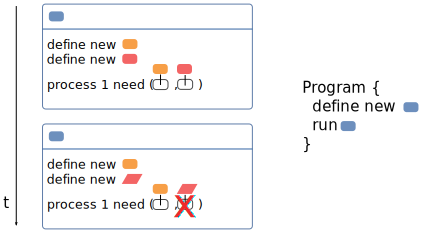
\includegraphics[width=.7\linewidth]{composants_principes_a.pdf}
  	\label{subfig_decouplage:a}}\qquad
  \subbottom[]{
	
\includegraphics[width=.8\linewidth]{composants_principes_c.pdf}
  	\label{subfig_decouplage:b}}
  \subbottom[]{
	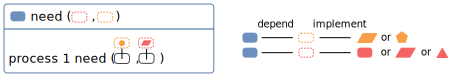
\includegraphics[width=.8\linewidth]{composants_principes_d.pdf}
  	\label{subfig_decouplage:c}}
 \end{sidecaption}
\end{figure}


Si on recontextualise ces principes à notre problèmatique, les classes de composants nécessaire à l'execution minimale d'un algorithme évolutionnaire dans MGO sont décrites dans la figure \ref{fig:cake_classe}, et s'appuie sur le travail déjà décrits de la communauté pour unifier la description des algorithmes.


\begin{figure}[!htbp]
	\begin{sidecaption}[fortoc]{Classe de composants nécessaires pour l'execution d'un EC.}[fig:cake_classe]
		\centering
		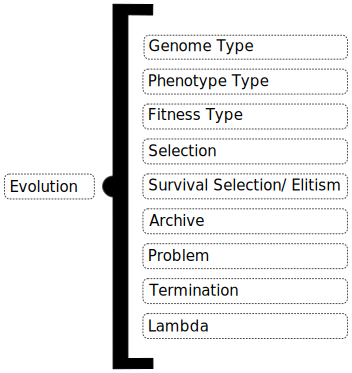
\includegraphics[width=0.7\linewidth]{cake_example.pdf}{
		}
  \end{sidecaption}
\end{figure}

Chacune de ces classes de composants est définit comme nécessaire pour le fonctionnement d'un algorithme d'évolution, dont la mise en dynamique du comportement générique est implémenté dans le composant Evolution. Tant que l'utilisateur n'aura pas fourni un composant compatible avec chacun de ces types de composants, alors le composant Evolution ne pourra pas s'executer. Le programme est définit comme un texte à trou, les boites sont bien placés, et le programme prêt à être executé suivant cet ordre, seulement ce n'est qu'un patron, une image, et cet ensemble de boite dont seule une partie de la logique à été intégré, doit encore être complété. C'est un peu comme un puzzle dans lequel il manque des pièces, vous devez soit créer de nouvelle pièces, soit retrouver les pièces qui respectent la forme de chaque trou pour que le puzzle soit de nouveau complet. 

L'inversion de controle détaillé dans les paragraphes précédents se matérialise de nouveau ici au travers du fait que c'est l'utilisateur qui définit sa composition, en s'assurant avec l'aide des instructions du programmes que les dépendances propres au fonctionnement de chacun des composants sont bien fournies. Tout programme ne remplissant pas les conditions renverra un message d'erreur à son execution. En ce sens MGO est probablement plus un \textit{framework} qu'une librairie logicielle \Anote{martin_fowler}. L'avantage d'une telle approche c'est que l'application peut être livrée avec un vaste catalogue de pièce correspondant à chaque emplacement, laissant à l'utilisateur la possibilité de choisir sa propre combinaisons, voire même de créer ses propres pièces si il estime quel sont manquantes. 

Ils existent différentes techniques pour que cette technique puisse être mise en oeuvre, mais en Scala, l'implémentation la plus courante et la plus utilisé est connu sous le nom de \foreignquote{english}{Cake Pattern}, \foreignquote{english}{Scalable Component Abstractions} ou encore \foreignquote{english}{Component Based Dependency Injection}, accessible nativement dans le langage car pensé et implémenté par son créateur Martin Odersky.

Le défaut de cette technique, c'est qu'il rend la lecture du code source plus difficile, du fait de ce morcellement dans l'appel des différentes fonctions.


\subsubsection{La mise en oeuvre du couplage MGO - openMOLE }

Le choix est fait ici de développé une librairie MGO utilisable de façon indépendante, ou de façon couplé à openMOLE. 

Les objectifs motivant la construction d'une nouvelle librairie sont les suivants : 



L'étape suivante est do nc le couplage de cette librairie avec openMOLE 


Martin Oderskys’


\begin{minted}[linenos=true,frame=single,fontsize=\footnotesize]{scala}
import fr.iscpif.mgo._
import math._
import util.Random

trait ZDT4 extends GAProblem with MGFitness {

  def min = Seq.fill(genomeSize)(0.0)
  def max = 1.0 :: Seq.fill(genomeSize - 1)(5.0)

  type P = Seq[Double]

  override def express(g: Seq[Double], rng: Random) = Seq(f1(g), f2(g))
  override def evaluate(p: P, rng: Random) = p

  def f1(x: Seq[Double]) = x(0)
  def f2(x: Seq[Double]) = g(x) * (1 - sqrt(x(0) / g(x)))
  def g(x: Seq[Double]) =
    1 + 10 * (genomeSize - 1) + (1 until genomeSize).map 
    { i => pow(x(i), 2) - 10 * cos(4 * Pi * x(i)) }.sum
}
}
\end{minted}

\section{Une brique logicielle dédiée à la visualisation de résultats}




%% -*- root: These.tex -*-

\section{SimpopLocal}
\label{sec:simpopLocal}

%% -*- root: These.tex -*-

\section{MicMac}
\label{sec:micmac}

\printbibliography[heading=subbibliography]

\appendix

\chapter{Historique du paradigme systémique}

\subsection{Retour sur la fondation et les apports du \enquote{paradigme systémique} au début du XXème siècle}
\label{ssec:systemique}

De la même façon que les épistémologues des sciences comme ici Olivier Orain \autocite{Orain2001}, l'auteur ne détaillera pas ici une approche inter-disciplinaire de la notion \footnote{Au sens donné par Piaget, voir note de bas de page \autocite {Orain2001}} de \enquote{système}, difficile à envisager dans un cadre global car sa diversité d'acceptation est fonction, d'une part de la rapide évolution de cette notion depuis les années 1940, et d'autre part la règle définissant l'acceptation de cette \textit{notion} dépend non seulement de la variabilité inter-disciplinaire, mais aussi intra-disciplinaire. Le terme \enquote{approche systémique} est alors proposé par \autocite{Orain2001} pour incarner cette diversité d'intégration par les disciplines des sciences sociales de la \enquote{théorie systémique} ou \enquote{systémique}.

La complexité d'approche caractéristique de cette notion est pour Jean Louis Lemoigne grandement lié à la reconstruction épistémologique \textit{a posteriori} de ce qu'il appelle \enquote{paradigme systémique}. Une acceptation qui parait d'autant plus justifié tant l'étude exhaustive de la ramification qui découle du concept est impossible, et sans rentrer dans les détails de querelles entre les différentes chapelles, il est acceptable de voir cette construction comme un processus de raffinement cumulatif. \hl{a dire mieux}

\subsubsection{La Cybernétique}
\label{ssubsec:cybernetic}

\paragraph{Des outils pour penser une nouvelle causalité}

Une des branches communément admises comme fondatrice du mouvement tient dans l'organisation des conférences de Macy entre 1942 à 1953. Celle ci sont considérés comme un des tout premier regroupement interdisciplinaire et marque une période de changement profond dans l'histoire des sciences en général, et particulièrement en science sociale. Celles ci vont réunir pendant plusieurs années autour d'une même table des acteurs majeurs des sciences physiques et sociales pour discuter autour de régularités communément observés, avec pour idée la construction d'un savoir commun que l'on pourra alors qualifier de trans-disciplinaire.

Les conférences naissent suite à la rencontre entre un mathématicien réputé au MIT N. Wiener, un neurobiologiste A. Rosenbluch, et un ingénieur électronicien J.Bigelow qui vont opérer un rapprochement entre l'homme et la machine entre 1942 et 1946 (pour rappel le premier ordinateur ENIAC est opérationel en 1946) par le biais de groupes inter-disciplinaires chargés d'explorer ce \textit{no man's land} à l'interface des deux disciplines.

Plusieurs \enquote{outils} dérivent de ces premiers séminaires organisés dès 1942 à la Josiah Macy, Jr. Foundation : la notion de \enquote{boite noire} ou système téléologique fonctionel, et la notion de \textit{feedback} ou causalité circulaire, avec pour objectif principal l'étude de l'homéostasie introduite auparavant par les travaux pionniers du physiologiste Walter Cannon en 1926.

Si la notion d'homéostasie pour des organismes vivants apparaît pour la première fois cité par Claude Bernard 1865, celle ci est reprise et étendue par Walter Cannon en 1932 dans le livre \textit{The Wisdom of the Body} \autocite{Cannon1932} comme « l’ensemble des processus organiques qui agissent pour maintenir l’état stationnaire de l’organisme, dans sa morphologie et dans ses conditions intérieures, en dépit de perturbations extérieures ». Ainsi dans le cadre de son application biologique cette rétro-action permet de décrire un certain nombre de mécanisme à l'oeuvre dans une cellule en interaction avec son environnement qui tente de maintenir de façon stable dans son milieu la concentration d'éléments comme les ions, la glycémie, etc.

L'attention des discutants dans ces premier séminaire porte donc avant tout sur l'ubiquité du concept et la pertinence de son transfert hors des systèmes biologiques. Wiener fait alors un rapprochement décisif entre les problématiques de calcul de trajectoire en balistique et des maladies nerveuses ayant pour symptôme l'ataxie. De ces discussions émergent alors un même schéma explicatif qui semble à la fois convenir à ces problématiques, la \enquote{causalité circulaire}. \autocite[774]{Pouvreau2013, Rosnay1975}

L'approche néo-béhavioriste retenue par les discutants \enquote{consiste à étudier un objet comme une \enquote{boite noire}, par l'examen de l'extrant de l'objet [i.e tout changement produit dans son environnement] et des relations entre cet extrant et l'intrant [i.e tout événement externe qui modifie l'objet]} \autocite{Pouvreau2013} En adoptant cette approche, le \enquote{comportement} d'une entité est perçu \enquote{comme tout changement extérieur détectable de cette entité par rapport à son environnement} , et par téléologique il faut entendre un comportement \enquote{finalisé} c'est à dire déterminé par un mécanisme de \enquote{rétroaction} négative. De la connaissance de ces entrants et de ces sortants, on peut en déduire qu'il existe une retro-action négative ou positive, ou \textit{feedback} permettant de décrire progressivement le système de commande de la boite noire.

L'introduction de cette \enquote{causalité circulaire} est pour l'époque loin d'être anodine car elle remet en cause le schéma classique linéaire cause \textrightarrow conséquence, qui se traduit dans le temps par la relation avant \textrightarrow après, la cause étant irrémédiablement suivi d'une conséquence. La possibilité de causalité circulaire, positive ou négative, brise ce schéma, et ne permet plus d'isoler un ordre entre cause et conséquence, c'est le problème de \enquote{la poule et de l'oeuf}. En réintroduisant la poursuite d'un but, on injecte une autonomie, une spontanéité, une dynamique entre objets qui était jusque là absente de la causalité linéaire déterministe.

Appliqué à un système servo-mécanique, la stabilité de celui-ci suppose la capacité à anticiper et à annuler les agressions extérieures par une capacité de régulation (flexibilité) qui repose plus alors sur la dynamique des interactions que sur la structure physique en place (rigidité), un mode de fonctionnement impossible si on se place dans le cadre de la \enquote{pensée classique} de l'époque.

%Dans "Behavior, Purpose and Teleology", le terme téléologie est à ce titre utilisé comme un synonyme de "l'objectif controllé par la rétroaction".\footnote{wikipedia}

\paragraph{La réintroduction du concept de \enquote{téléologie}}

Avec la mise en place d'une classification de ces comportements, et en prenant distance du concept de \enquote{causalité finale} qui lui était rattaché, les auteurs espèrent ainsi redorer le concept de téléologie, renouant avec la reconnaissance de l'\enquote{importance du but} qui avait disparu avec la mise au ban de ce concept. Reprenant les explications de \autocite[776]{Pouvreau2013}, celui-ci cite \autocite[23-24]{Rosenblueth1943} \enquote{[...] Puisque nous considérons la finalisation comme un concept nécessaire afin de comprendre certains modes de comportement, nous suggérons qu'une étude téléologique est utile si elle évite les problèmes de causalité et se limite à s'attacher à l'étude du but [...] Le comportement téléologique devient synonyme de comportement contrôlé par une rétroaction négative et gagne donc en précision par une connotation suffisamment restreinte.} La finalité est reintroduite via le concept de \enquote{téléologie}, mais elle est libéré de la notion de \enquote{causalité} qui lui était autrefois associé. Elle redevient l'étude des comportement associé à un but, dont l'importance ne peut plus être nié, et redevient compatible avec le concept autrefois opposé de déterminisme.\footnote{Pour donner un exemple peut-être plus parlant, l'étude en biologie des comportement oeuvrant dans la formation d'un organisme par une méthode téléologique n'empêche pas l'usage d'un cadre de pensée déterministe  correspondant à la formation d'un même organisme à partir d'un même code initial (un déterminisme largement remis en cause depuis, voir par exemple \href{http://www.nytimes.com/2014/01/21/science/seeing-x-chromosomes-in-a-new-light.html?ref=science&_r=0}{New York Times} )}

De ces discussions deux articles fondateurs à la fois des sciences cognitives \autocite[23]{Dupuy2000} et de la cybernétique vont être publiés : \textit{Behavior, Purpose and Teleology}ou Rosenblueth, Wiener, et Bigelow \enquote{ propose de déconstruire la distinction entre action volontaire et acte réflexe, en assimilant la volonté à un mécanisme de rétro-action (\textit{feedback})}; et \textit{A logical calculus of the ideas immanent in nervous activity} où McMulloch et Pitts donne \enquote{une base purement neuroanatomique et neurophysiologique au jugement synthétique \textit{à priori}, et de donner ainsi une neurologie de l'esprit}

\paragraph{ Les limites du transfert des concepts aux sciences sociales}

\subparagraph{Introduction aux sciences sociales}
Parmis les auteurs de ces premiers séminaires organisés entre 1942 et 1944 figurent deux représentant des sciences sociales, Gregory Bateson et Margaret Mead. Enthousiastes, il vont rapidement trouver dans l'étude des concepts développés dans ce premier séminaire (1942) un écho à leur propre travaux sur la dynamique sociale, la notion d'homéostasie n'étant qu'un nouveau mot permettant de rassembler des travaux existants déjà au fait de ces phénomènes. Cette mise au jour de problématiques commune entre le biologique et le mécanique permet d'envisager la construction d'un référentiel lui aussi commun; une prise de conscience qui va amener les auteurs du cercle de réflexion initial à envisager rapidement l'élargissement de celui-çi à l'ensemble des acteurs des sciences sociales.

La suite des conférences de Macy (1946-1952) sera organisés par Arturo Rosenbluch et son ami Warren McCulloch, un autre neurobiologiste. Cette ouverture vers les sciences sociales est timide dans un premier temps, et ce n'est qu'à la 2ème conférence en octobre 1946 sur une suggestion de Lazarsfeld que les conférences concrétise cette ouverture dans le cadre d'un sous séminaire intitulé \textit{Téléogical Mechanisms in Society}. La 4ème conférence acte cette ouverture et introduit pour la troisième fois de suite une modification de l'intitulé, avec cette fois ci l'adjonction d'une dimension sociale à un objet d'étude, qui apparaît encore à cette date difficile à définir : \enquote{la causalité circulaire et des mécanismes de \textit{feedback} dans les systèmes biologiques et sociaux}. Le terme \textit{Cybernetics} est pour la première fois introduit dans les séminaires par Wiener en 1946. Il faut toutefois attendre 1949 et la septième conférence pour que sous l'influence d'un nouveau participant nommé H. Von Foerster, ce terme chapeaute de façon définitive les prochains intitulés de séminaires. Au final, ces dix séminaires vont participer de l'émergence de la \enquote{science cybernétique} en \enquote{permettant l'échange effectif de savoir et d'experiences, tant entre les disciplines qu'entre les sciences et la société}, réalisant par là un des objectifs annoncé par Wiener et Rosenbluch dans leur classification, faisant de la cybernétique une \enquote{[...] science générale des systèmes à comportement finalisé ayant principalement pour objet ceux dont le comportements est \enquote{téléologique} } \autocite{Pouvreau2013}

\subparagraph{Des biais mécanisistes mettent en échec ce premier transfert}

Wiener mais aussi d'autre acteurs de la cybernétique ont vus assez tôt tout l'intérêt que pourrait apporter l'utilisation et le transfert d'outils comme \enquote{la boite noire}, ou le principe de régulation par \enquote{rétro-action} une fois appliqué à l'étude des interactions dans les systèmes sociaux. Mais les difficultés d'applications et les critiques ont rapidement mis à mal cet objectif trans-disciplinaire, pour plusieurs raisons qui tiennent : d'une part à l'existence de restriction mathématiques remettant en cause la scientificité des résultats obtenus : (a) les statistiques sur le long terme étant difficile à obtenir (b) la difficulté à minimiser la distance entre observateur et phénomène observés, et donc le biais qui s'applique aux données dans un tel cadre; et d'autres part au réductionnisme et le biais mécanicistes touchant la vision de certains acteurs des conférences de Macy  : \enquote{[...] la vie était pensée comme un dispositif de réduction d'entropie ; les organismes et leur associations, en particulier les hommes et leurs sociétés, l'étaient comme des servomécanismes ; et le cerveau comme un ordinateur} \autocite[784]{Pouvreau2013}

\autocite[782]{Pouvreau2013} explique très bien les limitations qui font  de l'extension de la cybernétique au sciences humaines une simple \enquote{[...] ressemblance superficielle au niveau du formalisme. Ne serait-ce que parce que dans un système tel que conçu par la \enquote{première} cybernétique, par définition fermé à l'information, la téléologie ne peut qu'être confinée au cercle d'un but déterminé; et que pour cette raison, ce modèle ne permet pas de comprendre de quelle manière un système peut être amené à redéfinir ses buts à partir de ses interactions avec son environnement, la pertinence d'une téléologie relative à des buts \textit{intentionels} restant donc intacte en sciences humaines}.

\subsubsection{La GST ou la théorie des \enquote{systèmes ouverts}}
\label{ssubsec:gst}

Cette incapacité de la première cybernétique à coller aux problématique des systèmes sociaux va trouver un écho plus positif dans un courant qui se développe en parallèle du mouvement cybernétique. Ce mouvement fondé par le biologiste Ludwig Von Bertalanffy en 1937 peut être considéré comme la deuxième branche venant enrichir le paradigme systémique. Tout en apportant de nouveaux concepts, celui ci va se positionner de façon critique par rapport à la \enquote{première cybernétique} tout en englobant par la suite les autres innovations qui proviendront de ce courant, Asbhy jouant le rôle important de médiateur entre ces deux courants.\autocite[]{Pouvreau2013} De cette prise de position va peu à peu découler la construction d'une théorie établissant une méthodologie logico-mathématique à vocation unifiante, accessible à n'importe quel champs disciplinaire pour décrire les lois de structure similaires (isomorphe). \autocite{LeMoigne2006a}.

Ainsi rapporté par LeMoigne en 1977, cette \enquote{vision stupéfiante est celle d'une une théorie générale de l'univers, du système universel} \autocite[59]{Lemoigne1977}. Le mot \enquote{Vision} est ici quasi synonyme de \enquote{Révélation}, car elle amène à voir une tout autre approche du réel pour qui s'en rapporte. Ainsi selon les mots même de Bertalanffy, \enquote{De tout ce qui précède se dégage une vision stupéfiante, la perspective d'une conception unitaire du monde jusque-là insoupçonnée. Que l'on ait affaire aux objets inanimés, aux organismes, aux processus mentaux ou aux groupes sociaux, partout des principes généraux semblables émergent} \autocite[59]{Lemoigne1977} \autocite[220]{Bertalanffy1949}. Une idée déjà existante dans la maxime célèbre de Claude Bernard en 1885, remise au gout du jour par \autocite{Lemoigne1977}, celle-ci résume toute la souplesse offerte par cette notion d'un point de vue de la modélisation :  \enquote{Les systèmes ne sont pas dans la nature mais dans l'esprit des hommes}

Cette théorie nommé \textit{General System Theory} (GST) est évoqué pour la première fois en public en 1937-38 par Bertalanffy, s'ensuit alors la rédaction d'une première ébauche en 1950, et il faudra attendre 1968 pour qu'un ouvrage titré \textit{General System theory: Foundations, Development, Applications} proposent une synthèse de toutes les avancées. La durée de développement de cette théorie n'est pas anodine, et si on en croit Pouvreau \autocite{Pouvreau2013} qui a analysé en détail la très vaste littérature associé à cette thématique, cette théorie n'en est pas vraiment une en réalité. En effet l'état inachevé du projet de Bertanlanfy laisse plus à penser qu'il s'agit là d'un \enquote{projet}, et c'est à ce titre que Pouvreau préfère employer le terme de \enquote{systémologie générale} pour désigner ce qu'il définit alors comme \enquote{le \textit{projet} d'une \textit{science de l'interprétation systémique} du \enquote{réel} } \autocite[9]{Pouvreau2013}. L'hypothèse défendu par Pouvreau étant que cette \enquote{[...]science de l'interprétation systémique du \enquote{réel} se caractérise en fin de compte comme une herméneutique, au sens où elle a pour vocation d'élaborer à la fois les moyens de construire des interprétations systémiques d'aspects particulier du \enquote{réel} sous la forme de modèles théoriques spécifiques et les moyens d'interpréter à leur tour de tels modèles comme des déclinaisons de modèles systémiques théoriques d'un degré de généralité supérieur.}\autocite[9-10]{Pouvreau2013}

Mais avant de même de fonder ce projet unifiant qui par la suite va rayonner et être absorbé (non pas sans déformation ..) dans un grand nombre de disciplines, dont la géographie, il est intéressant de rappeler comment la théorie biologique de Bertalanffy a participé de la formation de grandes notions comme l'\enquote{équifinalité} ou l'\enquote{auto-organisation}, des notions aujourd'hui communément admises comme fondatrice du paradigme actuel de la \enquote{complexité}.

Bertalanffy poursuivant depuis 1937 avant tout cet objectif de dépasser la compréhension des systèmes biologiques  englué jusque alors dans une dualité opposant les \enquote{vitalistes} et \enquote{mécanistes}. La synthèse de ces travaux est organisé dans une \enquote{biologie organismique} qui fonde une troisième voie visant d'une certaine manière la réconciliation entre les deux approches \autocite[55-56]{Lemoigne1977} \autocite[258]{Bertalanffy1949}. Avec cette nouvelle biologie théorique il s'agissait donc d'incarner \enquote{l'avenir de la biologie" en établissant via la mobilisation de moyen scientifique (analyse et analogies physico-chimique et mathématique du vivant) écartant la métaphysique/psychiques, un programme de recherche des \enquote{loi systémiques ou d'organisation à tous les niveaux de la nature vivante} entendues comme \enquote{l'explication de l'harmonie et de la coordination des processus à partir de la dynamiques des forces qui leur sont immanentes}}\autocite[456]{Pouvreau2013}. Principalement \enquote{ordonnées en direction de la conservation de la totalité}\autocite[440-458]{Pouvreau2013} dans une \enquote{tendance à une complication croissante}, cette \enquote{Gestalt organique} de la théorie \enquote{organismique} de Bertalanffy place \enquote{l'Organisation} des processus comme une véritable problématique de recherche, et met de coté la question de la \enquote{finalité} du vivant.\autocite[455-457]{Pouvreau2013}

Déjà tout à fait conscient que \enquote{le tout est plus que la somme des parties} Bertalanffy admet que l'étude des mécanismes physico-chimiques des processus vitaux tient plus d'une heuristique de recherche, une \enquote{méthode téléologique qui permet \enquote{d'examiner jusqu’à quel point le caractère de conservation de la totalité se manifeste dans les processus qui se déroulent en eux}} sans jamais arriver à en donner une complète description.\autocite[464]{Pouvreau2013}

Cette \enquote{biologie théorique organismique} (également appelé de façon synonyme par Bertalanffy \enquote{théorie systémique du vivant}) montre en bien des points toutes les prémisses d'une pensée systémiste et non réductionniste qui dépasse déjà largement le cadre seul de la biologie, et cela même avant 1937 et l'introduction de \enquote{systèmes ouvert} \autocite[499]{Pouvreau2013} qui ont fait la renommée de l'auteur.  Cette \enquote{biologie organismique} de Bertalanffy, bien évidemment construite sur les acquis et l'aide de bien d'autres de ces contemporains (voir \autocite{Pouvreau2013}, arrive à maturité en 1937 \autocite[14]{Pouvreau2013}, et présente déjà à ce stade tout les traits d'une première \enquote{systémologie restreinte}, qui va servir d'\enquote{antichambre} à la formation de la future \enquote{systémologie générale} (la première évocation publique date de 1945, mais des traces indirectes de ses premiers discours semblent remonter à 1937).\autocite[670]{Pouvreau2013} de Bertalanffy.

% D'abord on fait le point sur les principes (ce qui suppose de faire une grosse parenthèse avec tout ce que l'on a décrit sur la thermodynamique) et ensuite on peut passer à la critique, évoquant l'équifinalité et la hierarchisation de processus qui permet de recentrer aussi l'étude des boites noires.

L'articulation entre les deux \enquote{principes organismiques} qui fondent sa théorie apparaît de façon très claire dans une première définition du vivant en 1932, ici cité dans sa version telle que raffinée par Bertalanffy en 1937, date à laquelle selon

%Définition des deux principes organismiques !?

Le premier principe théorique \enquote{organismique} de Bertallanfy s'appuie sur le principe biologique fondamental qu'il a énoncé dès 1929 avec la \enquote{conservation du système organique en équilibre dynamique}. Un équilibre qui parait statique d'un point de vue extérieur, mais qui est en réalité dynamique car son existence même est basé sur la remise en jeu permanente d'une partie du travail effectué par la cellule pour maintenir le système organique loin de l'équilibre \enquote{vrai} (physique, c'est à dire celui qui correspond à une mort thermique, ou chimique qui ne peut pas produire non plus de travail à l'équilibre). Un \enquote{équilibre de flux} qui ne peut être réalisé que parce que l'organisme n'est ni un système fermé, ni un système statique, mais un système dont l'ordre et l'organisation (def à valider ici) est fondé sur un travail issue d'un \enquote{flux} de matière et d'énergie résultat d'une transaction à double sens avec son environnement. \autocite[472]{Pouvreau2013} Je me permettrai de citer ici Morin, qui reprenant Héraclite, évoque très bien cet antagonisme à l'oeuvre dans les systèmes organiques, mais aussi par extension sociaux \enquote{Vivre de mort, mourir de vie} : \enquote{ ne vivons-nous pas de la mort de nos cellules qui vieillissent et se décomposent pour laisser la place à des cellules jeunes ? [...] La vie et la mort sont certes deux ennemies fondamentales, mais la vie lutte contre la mort en utilisant la mort. Néanmoins, il est tuant de se régénérer en permanence. C’est épuisant. Finalement, on mveurt à force de rajeunir. On meurt de vie. } \autocite{MorinXX}

% Critique cybernétique
Le principe d'\enquote{équilibre des flux}, même si il peut être rapproché du concept d'\enquote{homéostasie} définit par les tenants de la \enquote{première Cybernétique} (en analogie avec les systèmes mécaniques) comme la \enquote{conjonction des processus par lesquels, nous autres, être vivants, résistons au courant général de corruption et de dégénérescence} est trop généraliste pour application en tant que tel à toute les notions de régulations organiques. \autocite[194]{Morin1977} \autocite{Wiener1950}. L'\enquote{homéostasie} tel que définit par Wiener dans le cadre de la Cybernétique s'avère en réalité être un mécanisme de régulation organique parmi tant d'autres, tous n'étant pas basé sur le schème de rétro-action. A ce titre, la notion d'\enquote{homéostasie} pourtant quasi semblable dans sa définition à l'équilibre de flux dans un système ouvert, mobilise en réalité un tout autre fonctionnement que le schème de rétro-action Cybernétique, et tient plus de l'extension aux systèmes ouverts du principe dit de \enquote{Le Chatelier}. De la même façon la régulation intervenant dans le processus de croissance des organismes qui nécessite la régénération, et l'évolution des structures dans le temps n'est pas compatible avec l'ordre structural pré-établi des machines et le scheme de rétro-action promis par la Cybernétique. La vision \enquote{machinaliste} limité/biaisé des premiers cybernéticiens n'est donc pas satisfaisante pour une application aux systèmes organiques, dès lors qu'il faut accepter la constance non pas des structures mais des interactions entre les structures. Bertalanffy développe une classification plus complète de ces régulations qu'il considère selon le type de leur téléologie, et introduit le concept d'\enquote{équifinalité} comme téléologie dynamique moteur dans la construction et le maintien des systèmes organiques. Dans ce contexte, le principe d'équifinalité \autocite[131]{Pouvreau2013}, est ainsi évoqué pour la première fois comme la possibilité d'atteindre le même état finalisé à partir de trajectoires quelconques, un processus impossible dans le cadre de système fermé où les condition initiales définissent par avance l'état final. Ce faisant, Bertalanffy introduit la primauté de l'ordre dynamique sur l'ordre structurel et fait de l'équifinalité un concept qui dérive de l'ouverture des systèmes. \autocite[489]{Pouvreau2013} \autocite[647]{Pouvreau2013} Un exemple illustrant les effets de l'équifinalité dans les organismes vivants peut être montré avec le processus de division embryonnaire. Ainsi un organisme a qui ont impose la fragmentation, la régénération, ou des blessures d'unités biologiques élémentaires comme les gènes ou les chromosomes va de façon constante s'organiser suivant un plan pré-établi menant à la \enquote{constitution d'un tout}, autrement dit un organisme complet.

%Il nécessite un autre mode d'explication de processus téléologique, celui de la cybernétique s'avérant incompétent au regard du principe d'équifinalité observé dans les systèmes organiques.

% Bertalanffy s'appuie dans sa critique à raffiner sa classification des téléologies, ce qui lui permet d'introduire le concept d'équifinalité comme sous-type de téléologie dynamique, un type de processus de régulation qui selon lui ne peut pas être expliqué par les schèmes cybernétique initiaux, seulement capable de mobiliser le concept de finalité en regard d'une explication basé sur un arrangement structural pré-établi (une machine faites de composants) et non pas l'ordre  dynamique propres au système en équilibre de flux.

La combinaison des deux principes \enquote{organismique} menant à la théorie des \enquote{système ouvert en équilibre de flux} deux heuristiques de recherches \autocite[481]{Pouvreau2013}:
\begin{itemize}
\item La subordination du \enquote{principe de hierarchisation} à celui du \enquote{système ouvert en équilibre de flux}, autrement dit la genèse et le maintien de l’ordre hiérarchique d’un \enquote{système organique} est conditionné par l'existence d'un \enquote{système ouvert en équilibre de flux}
\item  La relation précédente est un principe ubiquitaire s’appliquant à tous ses niveaux
\end{itemize}

Cet idée sera particulièrement fructueuses une fois articulé avec le principe d'un enboitement des systèmes, l'accroissement du degré de liberté dans un système résultant de l'équifinalité.
 \autocite[38]{Bertalanffy1973} \autocite[786-788]{Pouvreau2013}

%Developpement rendu possible uniquement par l'apport des théories de la thermodynamique ... l'expression d'une trajectoire indépendamment de l'état final, celui ci n'est qu'un processus de régulation parmis d'autres, car ce même système organique est non seulement capable de maintenir son état mais choses plus importante, il permet surtout de produire de l'organisation, de la complexification.

% Relation avec science sociale ??
% => entéléchie /
Cette notion d'équifinalité reliant un niveau micro à un niveau macro pourra par la suite être transposé dans les système sociaux, le parallèle de l'individu comme acteur réflexif dans la société sera mobilisé par ?

De ce fait la Cybernétique n'est pour Bertalanffy qu'un cas particulier dans une systémologie dont il pense qu'elle peut être beaucoup plus universelle... ++ Homéostasie avec Ashby ? ++

Tel que définie, cette notion d'équilibre dynamique de Bertalanffy est bien différente de celle produites en physique et en chimie, qui se caractérise justement par l'absence de travail disponible, l'énergie disponible étant minimale. Pour que la permanence d'un ordre puisse être effective dans la théorie organismique, il faut qu'il y ai un échange, un flux d'énergie mais aussi de matière possible avec l'environnement; une différenciation qui amène Bertalanffy à développer dès 1937 une théorie des \enquote{systèmes ouverts}, la seule capable de s'appliquer également à des systèmes sociaux par la suite.

% Sur l'ouverture des systèmes
Pour mieux comprendre en quoi cette ouverture est importante pour l'application du paradigme systémique aux sciences sociales, il faut revenir quelques décennies en arrière pour définir les limitations des premier systèmes issue de la thermodynamiques, limitations qui par la suite ont irrigués les réflexions initiales des cybernéticiens tout autant que les motivations de Bertalanffy pour les dépasser dans le cadre de sa théorie \enquote{organismique}

La seconde loi de la thermodynamique esquissé par Carnot et formulé par Clausius en 1850 montre que l'energie calorifique ne peut se reconvertir, elle se \textit{dégrade} et perd son aptitude à effectuer un \textit{travail}. Clausius nomme \enquote{entropie} cette diminution irréversible de l'aptitude à se transformer et à effectuer un travail, propre à la chaleur.\autocite[35]{Morin1977} Prigogine dans la \textit{fin des certitudes} écrit à propos de l'entropie qu'elle \enquote{[...] est l’élément essentiel introduit par la thermodynamique, la science des processus irréversibles, c’est-à-dire orientés dans le temps.}

C'est Boltzmann, Gibbs et Planck qui vont par la suite faire le lien entre le niveau micro des particules et la notion de chaleur. Parce que la chaleur est caractérisé par l'agitation désordonné des molécules dans un systèmes, l'entropie devient plus qu'une simple réduction du travail, c'est aussi l'ordre et le désordre des molécules qui en est la cause. Cette transformation s'effectue avec création d'entropie, une \enquote{quantité de désordre} qui ne peut que croître dans le temps et cela jusqu'à atteindre une valeur maximale équivalente à ce nouvel état d'équilibre. De ce fait et de façon générale celle-ci définit comme évolution irréversible toute transformation réelle dans un système isolé (Système où la frontière est totalement imperméable : l'Univers est par définition un tout englobant) ou fermé (Système ou la frontière est perméable aux flux entrant ou sortant d'énergie mais imperméable aux échanges de matière : La Terre reçoit de l'énergie du soleil) partant d'un état non stable et se dirigeant vers un nouvel état stable.  Ainsi si on considère l'univers comme un méta-système isolé englobant tout les autres, alors ce second principe a pour corollaire que l'entropie de l'univers augmente vers un état de désordre maximal qui se traduit en définitive par une mort thermique.

L'intuition de cette possible analogie entre loi gouvernant systèmes physiques et biologiques est issues des réflexions menés par Boltzman, qui comme ces contemporains du XIX siècle est admiratif pour la récente théorie évolutive de Darwin \autocite[27]{Prigogine1996}. Celui ci tente alors un parallèle avec ses propres travaux sur la seconde loi de thermodynamique, que l'on retrouve dans une des fameuses citations présente dans son livre \enquote{second law of thermodynamic} : \enquote{ The general struggle for existence of living beings is therefore not a struggle for raw materials — the raw materials of all organisms in the air, water and soil are in abundance there — nor about energy, which in the form of heat, unfortunately, is contained abundantly [but unfortunately] [in]convertible in each body, but a struggle for entropy, which is available [disposable] by the transfer of energy from the hot sun to the cold earth.}

% Le sys ouvert/fermé , de la thermodynamique à la biologie ?
Le point de vue de Boltzmann est repris et théorisé par Alfred J. Lotka, un mathématicien, chimiste et statisticien qui va largement influencé par la suite Bertalanffy dans la formation de sa \enquote{systèmologie générale} \autocite[178]{Pouvreau2013} par ces études de la démographie des populations et des flux de matières dans le monde biologiques \autocite[545-546]{Pouvreau2013} , toutes deux usant largement des équations différentielles (un premisse d'isomorphisme mathématique applicable à diverses disciplines pour qui quiconque tente de rentrer dans le formalisme de Lotka, et par la suite Lotka et Volterra \autocite[550]{Pouvreau2013}). De la même façon que Bertalanffy par la suite, celui ci ignore sciemment les débats entre \enquote{vitalistes} et \enquote{mécanicistes}, et adopte un point de vue unificateur qui vise la réconciliation entre système physique et système biologique, et part à la recherche d'isomorphisme en s'appuyant sur le processus d'irréversibilité commun aux deux paradigmes : \enquote{[...] the law of evolution is the law of irreversible transformation; that the \textit{direction} of evolution [...] is the direction of irreversible transformations. And this direction the physicist can define or describe in exact terms. For an isolated system, it is the direction of increasing entropy.  The law of evolution is, in this sense, the second law of thermodynamics} \autocite[26]{Lotka1925}.

Dès 1922 \autocite{Lotka1922a} \autocite{Lotka1922b} Lotka une nouvelle théorie qui acte la capacité de capturer de l'énergie comme un optimum à atteindre guidant la sélection tel quel est décrite par l'évolution Darwinienne. Il est également l'un des premier à percevoir les limites des lois actuelle de la thermodynamiques pour expliquer les processus du vivants, ainsi \enquote{Tenant pour légitime de traiter les êtres vivants et leurs associations comme des systèmes physiques, Lotka insistait toutefois sur le fait qu’il s’agit de « systèmes ouverts » aux flux de matière et d’énergie (ainsi que Raymond Defay (en 1929) et Bertalanffy (en 1932) les qualifièrent plus tard), capables d’échapper à l’équilibre thermodynamique défini par un maximum d’entropie promis aux systèmes fermés par le Second Principe, et d’évoluer vers une structuration croissante.} \autocite[179]{Pouvreau2013}

En effet pour un système vivant, l'état d'équilibre tel que décrit pour des systèmes clos ou isolé, correspond à un état de mort cellulaire. Hors, il est prouvé empiriquement à cette période que les systèmes vivants évolue dans un environnement chimique en perpétuel évolution loin de l'équilibre, et sont de fait capable de maintenir un haut niveau d'organisation par l'échange d'énergie et de matière avec l'environnement. Autrement dit, il n'est pas possible de concevoir l'équilibration permanente des systèmes vivants comme le résultat d'une évolution entropique croissante \autocite[248]{Lemoigne1977}. Des résultats énoncés sous forme de loi en 1929 par Bertallanfy, qui fait de \enquote{la conservation de système organique en équilibre dynamique} un \enquote{principe biologique fondamental}, et qui deviendra plus tard dans sa théorie \enquote{organismique}, le premier principe de  \enquote{système ouvert} en \enquote{équilibre de flux}. \autocite[492]{Pouvreau2013}

Mais en voulant faire l'analogie entre ces deux systèmes, une question va rapidement se poser aux scientifiques. \enquote{Comment la progression irréversible du désordre pouvait elle être compatible avec le développement organisateur de l'univers matériel, puis de la vie, qui conduit à homo sapiens ?}, une question qui va engendrer la problématisation et un changement de point de vue radical. Comme le résume bien \textit{a posteriori} Morin dans son premier tome de \textit{La Méthode}, \enquote{A partir du moment où il est posé que les états d'ordre et d'organisation sont non seulement dégradables, mais improbables, l'évidence ontologique de l'ordre et de l'organisation se trouve renversée. Le problème n'est plus : pourquoi y a-t-il du désordre dans l'univers bien qu'il y règne l'ordre universel ? C'est : pourquoi y a-t-il de l'ordre et de l'organisation dans l'univers ? } \autocite[37]{Morin1977}

Avec de tel propos se pose alors rapidement la question des mécanismes à l'oeuvre dans le vivant qui permettrait en quelque sorte de rétablir l'universalité de la seconde loi thermodynamique. Bien qu'intuité par de nombreux chercheur comme Lotka ou Bertalanffy, il faudra attendre les années 1940 pour que s'amorce plus concrétement ce rapprochement entre paradigme évolutionniste et domaine de la thermodynamique, concrétisé par le partage des théories entre biologistes et physiciens, qui va se réaliser notamment sous le couvert des récents progrès de ce dernier, permettant l'émission de nouvelle hypothèses.

Reprenant l'acceptation d'un système ouvert, c'est le livre \textit{What is Life} de Schrödinger (1944) qui va marquer le plus les esprits, et soulève le mieux ce paradoxe à la croisée des deux théories. Deux choses au moins fascine celui-ci \autocite{Foerster1959}, d'une part l'existence d'un code héréditaire qui définit au niveau micro la formation, l'organisation d'organisme au niveau macro (le principe \enquote{order-from-order}), d'autre part l'étonnante stabilité de ce code héréditaire immergé à 310 Kelvin \autocite[47]{Schrodinger1944}, et qui ne répond donc pas au fameux principe statistique \enquote{order-from-disorder} établit précédemment par Boltzmann.

En inscrivant comme nécessaire l'existence d'un code génétique comme un plan guidant l'évolution (tout comme Bertalanffy qui développe des théories similaires à la même époque), il introduit avec son concept de d'"entropie négative" un principe qui rend de nouveau compatible la seconde loi de thermodynamique avec l'évolution des systèmes biologiques : \enquote{le physicien attribuait le maintien de l’organisme dans un état \enquote{ stationnaire } éloigné de l’équilibre vrai à sa capacité de se \enquote{ nourrir } d’\enquote{ entropie négative } grâce à son ouverture sur son environnement. Une \enquote{ néguentropie } interprétée comme une \enquote{ création d’ordre à partir d’ordre } -- l’organisme créant un ordre spécifique à partir de la matière déjà ordonnée, structurée d’une manière déterminée mais devant être transformée pour ses besoins énergétiques, qu’il trouve dans son environnement} \autocite[502]{Pouvreau2013} Autrement dit, le maintien de l'organisation est un équilibre dynamique, un jeu à somme nulle où la création d'entropie est annulé par la capacité des organismes à transformer l'énergie, l'ordre puisé dans l'environnement pour maintenir ce degré d'organisation, un processus qualifié de néguentropique. Ce concept, déjà difficile à accepter tel quel dans sa généralité \autocite[225]{Lemoigne1977} va par la suite être raccroché à théorie de l'information de Shannon après son introduction en 1948 dans le microcosme Cybernétique. L'introduction de cette théorie étant un autre moment fort (avec la thermodynamique) ayant inspiré de nombreux développement dans la cybernétique. Mais les tentatives d'unification entre les deux théories débouche sur deux rapprochement possible, avec d'une part la qualification d'une \enquote{information pensé comme quantité physique} ou d'autre part l'expression des \enquote{quantité physique pensé comme de l'information}, selon que l'on adopte le point de vue de Wiener ou de Brilloin 1956 (auteur de la néguentropie qui associe qui associe \enquote{information} et principe de négentropie ). Ces points de vues font encore à l'heure actuelle l'objet de nombreux débats, certains voyant la physique de l'information comme un point de départ à creuser pour appeller une théorie de l'"organisation" \autocite[37-38]{Morin2005}, alors que d'autres n'y voient qu'un concept flou seulement basé sur la similitude des deux formules. Autant de ramifications naissent de ces positions, et leur présentation dépassent de loin le seul cadre d'étude de cette thèse, mais le lecteur pourra se référer au travail de \autocite{Triclot2007} pour mieux comprendre le point de départ d'un malentendu qui dure toujours /footnote{Voir par exemple la différence de ton qui existe entre le site http://www.eoht.info/page/Information+theory, mais aussi les notes de bas de pages de \autocite[277]{Lemoigne1977} }.

\autocite[482]{Pouvreau2013} Mais finalement plus que les idées développés par Shrödinger, la plupart étant déjà largement sous entendu dans les travaux des biologistes de l'époque, il semblerait plutôt que cela soit avant tout ce nouvel éclairage physiciste apporté à la biologie {REF}, et l'espoir déguisé (finalement non réalisé) de trouver de nouvelles lois physique à l'oeuvre dans la construction du vivant associé à la grande diffusion du petit livre dans le grand public qui amèna peut être de nombreux physiciens à ne plus ignorer les avancés dans ce domaine, notamment durant les années 1940 / 50, tel que Prigogine \autocite[77]{Prigogine1996}, Von Foerster, etc. \autocite[73]{Lemoigne1977}

Mais conscient des manquements et des reproches faites à son approche, alors incomplète, car focalisé sur la cinétique, celle ci n'est pas relié à une théorie plus explicatives sur les mécanismes energétiques à l'oeuvre justifiant l'existence de ces propriétés des systèmes vivants dans le cadre des systèmes ouverts. C'est les récents développements sur la \enquote{Thermodynamique des processus irréversibles} qui va introduire a posteriori la possibilité d'une thermodynamique des systèmes ouverts compatible avec l'approche de Bertlanffy. Des physiciens ayant participé à ces travaux sur la thermodynamique des systèmes ouverts loin de l'équilibre (Osanger, etc.) c'est les travaux de Prigogine  en 1946 \autocite{Prigogine1946} qui vont le plus attirer l'attention de Bertalanffy. Lorsque celui ci découvre vers 1948 ces récentes avancées qui semble faire parfaitement écho à ces travaux ( Prigogine n'hésitant pas à citer Bertalanffy comme un de ses modèles d'inspiration \autocite{Prigogine1996}), le rapprochement se fait assez rapidement et Bertalanffy n'hésite pas à promouvoir cette nouvelle thermodynamique comme le parfait support physique justifiant des principes qu'il a établi dans sa propre théorie des système ouvert en équilibre des flux ! \autocite[653-658]{Pouvreau2013}

Pas étonnant donc de voir Bertallanffy s'appuie sur les écrits de Schrödinger pour re-formuler et préciser ses premières intuitions,
+

Malheureusement le \enquote{théorème de Prigogine} de \enquote{minimum de production d'entropie} ne s'exprime que dans des conditions semblent il très drastiques \autocite[53]{Lebon2008} et limité à des systèmes très proche d'un état d'équilibre tel que le prouve les travaux de Denbigh : \enquote{ It is possible that certain reactions in biological systems may be sufficiently close to equilibrium for the rate of entropy production due to them to be very small. But in general it seems that the notion of minimum entropy production has no real significance as applied to chemical reaction in open systems [...] it is incorrect to regard the tendency of an open system to approach a stationary state as being determined by thermodynamic factors. The stationary state may or may not coincide with a state of minimum entropy production, according to whether the rates of the individual processes are linear functions of thermodynamic variables. In the above we have assumed this to be the case for diffusion (eqn. (ll)), but it is known not to be true for chemical reaction.} \autocite{Denbigh1952}

Hors l'état des systèmes biologiques est semble t il loin d'être proche d'un état d'équilibre thermodynamique.. Bertalanffy qui jusqu'à présent se contentait de relier les résultats à son programme organismique ne cache alors plus sa déception lorsque en 1953 il écrit \enquote{Un minimun de production d'entropie ne caractérise donc pas l'équilibre des flux dans les systèmes ouverts [...]}; autrement dit \enquote{la thermodynamique [...] ne nous dit jamais ce qui peut se passer dans un système, ce qui est permis [...] Et le problème de l'organisation progressive, la tendance néguentropique de l'évolution des organismes simples aux organismes compliqués, reste à présent non résolu.} Bien qu'ils n'abandonne pas l'idée de voir expliquer un jour sa théorie organismique par une théorie thermodynamique adapté, il abandonne en 1953 l'étude de la biophysique des systèmes ouverts et se consacre par la suite uniquement à la construction de sa théorie du système général.

Le fait est qu'il y a réduction d'entropie dans les systèmes en équilibre de flux, et qu'il y a maintient et augmentation du niveau d'organisation, sans que l'on sache pourquoi pour le moment dans le monde du vivant. Si l'analogie et le pont entre tissé entre physique et biologie semble donc encore soumis à questionnement, les travaux de Prigogine sur la thermodynamique des systèmes ouverts va continuer quand a elle à ouvrir bien d'autres perspectives, notamment dans les systèmes sociaux.

%paragraphe dimension reflexive auto-orga ...
Elle dépasser largement ce cadre, et appuie sur des bases physiques le concept d'"auto-organisation", une notion déjà introduite dans le mouvement cybernétique par Ashby, un homme clef dans la convergence des idées entre Cybernétique et GST.

Ashby, tout comme Von Foerster interviennent dans la création de la seconde cybernétique, et introduise une dimension réflexive aux débats.

Inspiré par Von Foerster, vont alors introduire un autre concept \enquote{d'order from noise}, totalement différent du \enquote{order-from-disorder} de Schrodinger.

TODO : Partie plus axé sur les changements de causalité ? (vient avant ou apres ici ?)

L'équifinalité

Un autre concept important est introduit par Ashby dans le mouvement Cybernétique, le concept d'auto-organisation, l'introduction du mot \enquote{auto} amorcant ainsi un virage réflexif qui annonce la seconde Cybernétique, piloté par Von Foerster.


%Des auteurs comme Prigogine en 1947 >> clairement inspiré par bertalanffy/ Schrodinger...  cf Pouvreau et internet
%Il fait le lien avec processus physique =>
%http://www.informationphilosopher.com/solutions/scientists/prigogine/
%http://www.informationphilosopher.com/solutions/scientists/schrodinger/

%http://en.wikipedia.org/wiki/Entropy_%28information_theory%29#Relationship_to_thermodynamic_entropy

C'est également à cette époque, que relayant les premiers travaux de Prigogine sur les systèmes dissipatifs, Bertalanffy va catalyser ainsi ces idées dans sa GST.

Ce procédé sera transféré au réel par Ashby, un autre cybernéticien qui travaillera dès 1946 à la mise au point d'une machine expérimentale capable de reproduire de façon mécanique cette dynamique de stabilisation face aux variations de son environnements. Nommé \enquote{homéostat} celle çi sera construite en 1948, et présenté aux conférences de Macy en 1952.

WIkipedia => L'implication de la cybernétique dans la systémique est historiquement plus liée au « deuxième mouvement cybernétique ». En effet, si selon Norbert Wiener la cybernétique étudie exclusivement les échanges d'information (car c'est « ce qui dirige » les logiques des éléments communicants d'où le mot cybernétique), dans son évolution qui engendrera la systémique, on réintègre les caractéristiques des composantes du système, et on reconsidère les échanges d'énergie et de matière indépendamment des échanges d'information.

La dégradation de l'énergie nécessaire pour maintenir une organisation implique l'irréversibilité des transformations.


The history of an open system is part of its structure, and Prigogine links open systems to irreversibility. Prigogine calls open systems dissipative. Put more simply, this means that matter does not tend to organise itself in a particular location unless there is some external energy source powering it. Evolution can be seen as matter organising itself.


The term \enquote{self-organizing} was introduced to contemporary science in 1947 by the psychiatrist and engineer W. Ross Ashby.[9] It was taken up by the cyberneticians Heinz von Foerster, Gordon Pask, Stafford Beer and Norbert Wiener himself in the second edition of his \enquote{Cybernetics: or Control and Communication in the Animal and the Machine} (MIT Press 1961).

Self-organization as a word and concept was used by those associated with general systems theory in the 1960s, but did not become commonplace in the scientific literature until its adoption by physicists and researchers in the field of complex systems in the 1970s and 1980s.[10] After Ilya Prigogine's 1977 Nobel Prize, the thermodynamic concept of self-organization received some attention of the public, and scientific researchers started to migrate from the cybernetic view to the thermodynamic view. WIKIPEDIA


Malgré les critiques soulevés de part et d'autres, du faite entre autre d'un objectif peut être un peu sur-évalué voire immodeste, celle ci aura un large écho auprès des sciences humaines, et notamment en géographie; d'abord anglo-saxonne \autocite{Haggett1965, Chorley1962}, puis par diffusion en France \autocite{Raymond}.



L'avénement de la deuxième cybernétique :
La régulation apparaît en effet comme un phénomène majeur chez les organismes vivants, puisqu’elle « retarde la dégradation de l’énergie et donc l’augmentation de l’entropie » (p 129), et associée au retard d’entropie et à la computation, elles forment l’essence même de la cybernétique


\printbibliography[heading=subbibliography]

\stopcontents[chapters]
